%%% master.tex --- 
%% \revision$Header: /Users/bob/SourceCode/Notes/ocaml-hacker.tex,v 0.0 2011/10/23 02:58:53 bob Exp$
\documentclass[svgnames,12pt,a4paper]{book}
\usepackage[latin9]{inputenc}
\usepackage[letterpaper]{geometry}
\geometry{verbose,tmargin=1in,bmargin=1in,lmargin=1in,rmargin=1in}


\usepackage{amsmath}
\usepackage{amssymb}
\usepackage{graphicx}
\usepackage{float}
\usepackage{array}
\usepackage{tikz}
\usepackage{longtable}
\usepackage{enumerate}
\usepackage{lmodern}
\usepackage[T1]{fontenc}
\usepackage{textcomp}
\usepackage{hyperref}
\usepackage{listings}
\usepackage{fancyvrb}
\usepackage{wasysym}
\usepackage[online]{suthesis-2e}
\usepackage{todonotes}
\usepackage{caption}
\usepackage{minted}


\usepackage{setspace}

\definecolor{MyDarkBlue}{rgb}{0,0.08,0.45}
\definecolor{lightgray}{rgb}{0.9,0.9,0.9}
\definecolor{lightlightgray}{rgb}{0.95,0.95,0.95}


%% begin listing configuration 
\lstset{
  % basicstyle=\footnotesize\ttfamily,
  basicstyle=\scriptsize,
  numberstyle=\tiny,
  % numbers=left,
  stepnumber=5,
  numbersep=5pt,
  tabsize=2,
  extendedchars=true,
  breaklines=true,
  keywordstyle=\color{blue}\bfseries, % to do
  stringstyle=\color{orange}\ttfamily, %to do
  identifierstyle=\color{teal},
  showstringspaces=true,
  showspaces=false,
  showtabs=false,
  % xleftmargin=17pt,
  framexrightmargin=5pt,
  framexbottommargin=4pt,
  % backgroundcolor=\color{lightgray}, % to do
  commentstyle=\color{red},% todo 
  % frame=lines,
  frame=bottom,
  backgroundcolor=\color{lightlightgray},
  framerule=1pt,
  % emph={square,root},
  % emphstyle=\underbar,
  %% language={[Objective]Caml},
}
\DeclareCaptionFont{green}{\color{green}}
\DeclareCaptionFormat{listing}{\colorbox[cmyk]{0.43, 0.35,
    0.35,0.01}{\parbox{\textwidth}{\hspace{15pt}#1#2#3}}}

\captionsetup[lstlisting]{format=listing,labelfont=green,textfont=green, singlelinecheck=false, margin=0pt, font={bf,footnotesize}}

%% end


\makeatletter

\makeatother


% \newenvironment{ocamlcode}{\Verbatim[fomartcom=\color{blue}]}{\endVerbatim}
% New commands serve as shorthand for frequently used command combinations.
% \newcommand{\ind}[1]{\mathbf{1}\left(#1\right)}
% \newcommand{\bx}{\mathbf{x}}
% \newcommand{\E}{\mathbf{E}}
% \DefineVerbatimEnvironment{ocamlcode}{Verbatim}{formatcom=\color{red},fontsize=\scriptsize}
% \DefineVerbatimEnvironment{bluetext}{Verbatim}{formatcom=\color{MyDarkBlue},fontsize=\scriptsize}
% \DefineVerbatimEnvironment{ocamlcode}{Verbatim}{formatcom=\color{blue},fontsize=\scriptsize}
% \lstnewenvironment{ocamlcode}
% {\singlespacing}{}


\usepackage{etoolbox}

\setlength\partopsep{-\topsep}
\addtolength\partopsep{-\parskip}
\addtolength\partopsep{0.5cm}


%% \AtBeginEnvironment{minted}{\fontsize{10}{10}\selectfont}


%% \AtBeginEnvironment{bluetext}{\singlespacing%
%%     \fontsize{10}{10}\selectfont}


%% \AtBeginEnvironment{inputminted[fontsize=\scriptsize, ]}{\singlespacing%
%%     \fontsize{10}{10}\selectfont}


\newcommand{\ChangeLine}[1]{%
\ifodd\value{FancyVerbLine}%
\textcolor{red}{#1}\else\textcolor{blue}{#1}\fi}


\newminted{ocaml}
{fontsize=\scriptsize,bgcolor=lightlightgray,
  frame=lines, framesep=2mm, numbersep=5pt,
  linenos}
\newminted{bash}
{fontsize=\scriptsize,bgcolor=lightlightgray,
  frame=lines, framesep=2mm, numbersep=5pt,
  linenos}

\lstnewenvironment{bluetext}
{\singlespacing\lstset{backgroundcolor=\color{lightgray}}}{}

\DefineVerbatimEnvironment{alternate}{Verbatim}%
{formatcom=\renewcommand{\FancyVerbFormatLine}{\ChangeLine},%
fontsize=\scriptsize,frame=lines}{}





% \includeonly{toolchain/ob}
\begin{document}

%% \documentclass{book}
%% \usepackage{graphicx}
%\usepackage{fancyvrb}
%% \begin{document}
\clearpage
%% temporary titles
% command to provide stretchy vertical space in proportion
\newcommand\nbvspace[1][1]{\vspace*{\stretch{#1}}}
% allow some slack to avoid under/overfull boxes
\newcommand\nbstretchyspace{\spaceskip0.5em plus 0.25em minus 0.25em}
% To improve spacing on titlepages
\newcommand{\nbtitlestretch}{\spaceskip0.6em}
\pagestyle{empty}
\begin{center}
\bfseries
\nbvspace[1]
\Huge
{\nbtitlestretch\huge
 FUN OF PROGRAMMING }


%% \newline
\nbvspace[1] 
\scriptsize \textit{the tao produced one \\
one produced two\\
two produced three\\
three produced all things\\ }

\small \textit{by}\\
\large \textit{hongbo zhang}\\[0.5em]

\nbvspace[1]
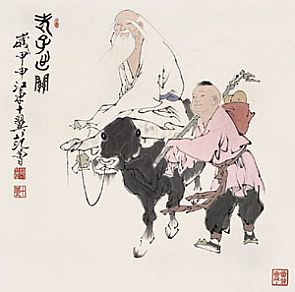
\includegraphics[width=4in]{./graphics/lao}

\footnotesize University Of Pennsylvania

\nbvspace[2]


\nbvspace[3]
\normalsize

%% Hongbo Zhang\\
\large
Work In Progress
\nbvspace[1]
\end{center}


\setcounter{tocdepth}{4}


%% \title{OCaml Hacks}
%% \author{Hongbo Zhang}
%% \maketitle


\prefacesection{Preface}
\begin{quotation}

  This is a book about advanced programming in Ocaml.  It's assumed
  that you are already familiar with the basic ideas of the different
  paradigms of programming, for example, functional programming,
  object-oriented programming, macro programming.

  I am a graduate student of University of Pennsylvania right now, I
  love programming and spend a lot of time digging different
  interesting languages and the underlying theories, including
  \textit{c,c++,ocaml,haskell,common lisp, perl} and know tiny bits
  about \textit{coq,prolog,python}.

  Haskell is the most elegant language that I ever used and is the
  language which brought me to the beautiful world of function
  programming, while Ocaml is the most productive one for me, since it
  supports multiple paradigms and Haskell's \textit{lazy evaluation}
  renders it impractical for real world programming. I love Haskell's
  all good parts except \textit{lazy evaluation}! Even for
  meta-programming, haskell's good support for generic programming
  makes it less painful compared with programming in camlp4(camlp4
  supports quasiquotation mechanism fully, however).

  Another interesting language is \textit{common lisp}, the most
  interesting book that I read about programming is \textit{Paradigms
    of Artificial Intelligence Programming: Case Studies in Common
    Lisp} which is written in \textit{common lisp}. Some other
  interesting books about \textit{lisp} are \textit{On Lisp} and
  \textit{Let Over Lambda}. \textit{Clojure} is a modern dialect of
  \textit{common lisp}, while its implementation is a bit weak at this
  time. Lisp's good part mainly lies in \textit{meta-programming}.
  However, from the point of view of mine, type safety is a really
  good tool to keep the quality of your software. And the good parts
  of lisp are largely incorporated by \textit{Haskell, OCaml}, it's
  not too hard to do meta programming in Ocaml, and sometimes it's
  even more convenient.

  Feel free to contact me if you found it
  interesting. \textit{hongboz\@seas.upenn.edu}
  
  To conclude, \textit{OCaml} is the most productive language at this
  time, and that's why I wrote this book.

  
  This is still a book in progress. Don't distribute it without permission.


\end{quotation}
\prefacesection{Acknowledgements}
\todo{write later}



\newpage

\tableofcontents
\listoftodos
\vspace*{1cm}

\newpage
\newpage 
\chapter{Tool Chain}

\section{Ocamlbuild}

The reason for \verb|ocamlbuild| in OCaml is to solve the complex scheme to
when building camlp4. But it's very useful in other aspects as well.

Your code is in the \verb|_build| directory. \verb|ocamlbuild| copies
the \verb|needed| source files and compiles them.  In \verb|_build|,
\verb|_log| file contains detailed building process. \verb|ocamlbuild|
automatically creates a symbol link to the executable it in the
current directory.  Hygiene rules at start up (.cmo, .cmi, or .o
should not appear outside of the \verb|_build|). Sometimes when you
want to mix c-stubs, you tag the .o object file \verb|precious| or
\verb|-no-hygiene|


Important Compile Flags 

\begin{spacing}{0.5}\small
\begin{tabular}{|c|c|}
\hline
option & comment \\
\hline
-quiet & \\
-verbose <level> & \\
-\textbf{documentation} & show rules and flags for a \textbf{specific} \verb|_tags| file
\\
-clean & \\
-r & Traverse directories by default\textit{true:traverse} \\
-I <path> & \\
-Is <path,...> & \\
-X <path> & \textit{ignore} directory \\
-Xs <path,...> & \\
-lib <flag> & link to ocaml library \textit{.cma} \\
-libs <flag,...> & \\
-mod <module> & link to ocaml module \\
-mods & \\
-pkg <package> & link to \textit{ocamlfind package} \\
-pkgs <...> & \\
-lflag  <flag> & ocamlc link flags \\
-lflags & \\
-cflag & ocamlc comple flags \\
-cflags & \\
-yaccflag &  Add to ocamlyacc flags, you can hack for \verb|menhir| \\
-yaccflags & \\
-lexflag & \\
-lexflags & \\
-pp & preprocessing flagss\\
-tag <tag> & add to default tags \\
-tags & \\
-show-tags & for \textit{debugging},\verb|ocamlbuild -show-tags target| \\
-ignore <module,...> & \\
-no-hygiene & \\
-no-plugin & \\
-just-plugin & just build myocamlbuild.ml \\
-use-menhir & \\
-use-jocaml & \\
-use-ocamlfild & \\
-build-dir & set \textit{build} directory (implies no-links)\\
-install-lib-dir <path> & \\
-install-bin-dir & \\
-ocamlc <command> & set the ocamlc command \\
-ocamlopt  & \\
-ocamldoc & \\
-ocamlyacc & \\
-menhir & set the menhir tool (use it after -use-menhir)\\
-ocamllex & \\
-ocamlmktop & \\
-ocamlrun & \\
--  & supply arguments \\
\hline
  \end{tabular}
\end{spacing}


Simple Examples

\begin{bluetext}
ocamlbuild -quiet xx.native -- args
ocamlbuild -quite -use-ocamlfind xx.native -- args
\end{bluetext}


You can pass flags to \verb|ocamlc| at compile time. i.e,
\verb|-cflags -I,+lablgtk,-rectypes|

You can link with \textit{ external} libraries. i.e,
\verb|-libs unix,num|.  You may need add the options below to make it
work if this not in OCaml's default search path
\verb|-cflags -I,/usr/local/lib/ocaml|
\verb|-lflags -I,/usr/local/lib/ocaml|


You can also build a library with specicfic modules included using
\verb|mllib| file

\begin{bluetext}
cat top_level.mllib    
Dir_top_level_util
Dir_top_level  
\end{bluetext}

Then you can \verb|ocamlbuild top_level.cma|, then you can use
\textbf{ocamlobjinfo} to see exactly which modules are compacted into
it.

\begin{bluetext}
ocamlobjinfo _build/top_level.cma | grep Unit  
Unit name: Dir_top_level_util
Unit name: Dir_top_level
\end{bluetext}

You can alo use  \verb|mlpack| file to do hierachical packing 
\todo{mlpack file}

You can also make use of \verb|_tags| file for convenience.  Every
source tree may have a \verb|_tags| file, and each target may have a
set of tags .
\begin{bluetext}
bash-3.2$ocamlbuild -show-tags test.ml

Tags for "test.ml":
  {. extension:ml, file:test.ml, ocaml, pkg_camlp4.macro, pkg_menhirLib,
     pkg_ulex, predefine_ulex.ml, quiet, syntax_camlp4o, traverse, use_menhir .}

bash-3.2$ ocamlbuild -show-tags test.byte
Tags for "test.byte":
  {. byte, extension:byte, file:test.byte, ocaml, pkg_menhirLib, pkg_ulex,
     program, quiet, traverse, use_menhir .}

bash-3.2$ ocamlbuild -show-tags test.native
Tags for "test.native":
  {. extension:native, file:test.native, native, ocaml, pkg_menhirLib,
     pkg_ulex, program, quiet, traverse, use_menhir .}

\end{bluetext}
%$

You can digest the output to get a general idea of how tags file work.
By preceding a tag with a minus sign, one can \verb|remove| tags from
one or more files.

The built-in \verb|_tags| file as follows:
\begin{bluetext}
<**/*.ml>   or <**/*.mli> or <**/*.ml.depends> : ocaml 
<**/*.byte> : ocaml, byte, program 
<**/*.native>: ocaml, native, program
<**/*.cma>:ocaml, byte,library
<**/*.cmxa>:ocaml,native,library
<**/*.cmo>:ocaml,byte
<**/*.cmx>:ocaml,native
\end{bluetext}
You can do some experiment do verify it, create a empty directory, and
make a dummy ml file, then type \verb|ocamlbuild -show-tags test.ml|,
you will get the output as follows 
\begin{bluetext}
Tags for "test.ml": {. extension:ml, file:test.ml, ocaml, quiet .}
\end{bluetext}

\verb|<**/*.ml>| means that \verb|.ml| files in \emph{current dir or
  sub dir}. A special tag made from the path name of the file relative
to the toplevel of the project, is automatically defined for each
file.  Just as above \verb|test.ml| will be tagged
\verb|file:test.ml|and also \verb|extension:ml|


Considering multiple directories:

Suppose our directory structure is as follows 
\begin{bluetext}
   |---bar
   |---baz
   |---foo
\end{bluetext}
Our tags file is 
\begin{bluetext}
<bar> or <baz> : include 
bash-3.2$ cat foo/main.ml
open Printf
let _ = begin
  print_int Barfile.i;
  print_int Bazfile.j;
end 
\end{bluetext}
%$
Here module \verb|Barfile| and \verb|Bazfile| lies in directries
\verb|bar,baz|. So, after typing ocamlbuild in
\verb|toplevel directory|, then your directory structure is as follows

\begin{bluetext}
   |-_build
   |---bar
   |---baz
   |---foo
   |-bar
   |-baz
   |-foo
\end{bluetext}

What \verb|ocamlbuild| did is explicit if you read \verb|_log|
\begin{bluetext}

bash-3.2$ cat _build/_log 
### Starting build.
# Target: foo/main.ml.depends, tags: { extension:ml, file:foo/main.ml, ocaml, ocamldep, quiet, traverse }
/opt/godi/bin/ocamldep.opt -modules foo/main.ml > foo/main.ml.depends
# Target: bar/barfile.ml.depends, tags: { extension:ml, file:bar/barfile.ml, ocaml, ocamldep, quiet, traverse }
/opt/godi/bin/ocamldep.opt -modules bar/barfile.ml > bar/barfile.ml.depends
# Target: baz/bazfile.ml.depends, tags: { extension:ml, file:baz/bazfile.ml, ocaml, ocamldep, quiet, traverse }
/opt/godi/bin/ocamldep.opt -modules baz/bazfile.ml > baz/bazfile.ml.depends
# Target: bar/barfile.cmo, tags: { byte, compile, extension:cmo, extension:ml, file:bar/barfile.cmo, file:bar/barfile.ml, implem, ocaml, quiet, traverse }
/opt/godi/bin/ocamlc.opt -c -I bar -I baz -o bar/barfile.cmo bar/barfile.ml
# Target: baz/bazfile.cmo, tags: { byte, compile, extension:cmo, extension:ml, file:baz/bazfile.cmo, file:baz/bazfile.ml, implem, ocaml, quiet, traverse }
/opt/godi/bin/ocamlc.opt -c -I baz -I bar -o baz/bazfile.cmo baz/bazfile.ml
# Target: foo/main.cmo, tags: { byte, compile, extension:cmo, extension:ml, file:foo/main.cmo, file:foo/main.ml, implem, ocaml, quiet, traverse }
/opt/godi/bin/ocamlc.opt -c -I foo -I baz -I bar -o foo/main.cmo foo/main.ml
# Target: foo/main.byte, tags: { byte, dont_link_with, extension:byte, file:foo/main.byte, link, ocaml, program, quiet, traverse }
/opt/godi/bin/ocamlc.opt bar/barfile.cmo baz/bazfile.cmo foo/main.cmo -o foo/main.byte
# Compilation successful.
\end{bluetext}

%$

So, you can see that \verb|-I | flags was added for each included
directory and their source was copied to \_build, \verb|foo| was copied
was due to our target \verb|foo/main.byte|. They are still flat
structure actually. Ocamlbuild still views each directory as source
directory and do santity check. Each source tree should still be built
using ocamlbuild, it's not easy to mix with other build tools. You can
add \verb|-I| flags by hand, but the relative path does not work. I
did not find a perfect way to mix ocamlbuild with other build tools yet.



You can also  group your targets \verb|foo.itarget, foo.otarget|
\begin{bluetext}
cat foo.itarget
main.native
main.byte 
stuff.docdir/index.html    
\end{bluetext}
Then you can say \verb|ocamlbuild foo.otarget|


For preprocessing either \verb|-pp| or tags \verb|pp(cmd ...)| 

For debugging and profiling either \verb|.d.byte, .p.native| or
\verb|true:debug|


To build documentation, create a file called \verb|foo.odocl|, then
write the modules you want to document, then build the target
\verb|foo.docdir/index.html|. When you use \textit{-keep-code} flag in
myocamlbuild.ml(\ref{myocamlbuild}), \textit{only} document of exposed
modules are kept, not very useful.  Add such a line in your
\verb|myocamlbuild.ml| plugin.
\verb| flag ["ocaml"; "doc"] & S[A"-keep-code"];| Or you can do it by
hand
\verb|ocamlbuild -ocamldoc 'ocamlfind ocamldoc -keep-code' foo.docdir/index.html|
\verb|ocamldep| seems to be \textbf{ lightweight}.  It's weird when
you have \verb|mli| file, \verb|-keep-code| does not work

\todo{Glob Patterns}




\textbf{With lex yacc, ocamlfind }


\verb|.mll .mly| supported by default, you can use menhir
\verb|-use-menhir| or add a line \verb|true : use_menhir|

Add a line in tags file
\begin{bluetext}
<*.ml> : pkg_sexplib.syntax, pkg_batteries.syntax, syntax_camlp4o
\end{bluetext}

Here \verb|syntax_camlp4o| is translated by
myocamlbuild.ml(\ref{myocamlbuild}) to \verb|-syntax camlp4o| to pass
to ocamlfind pkg needs \textbf{ocamlbuild plugin} support.


Examples with Syntax extension 
\begin{bluetext}
<*.ml>: package(lwt.unix), package(lwt.syntax), syntax(camlp4o) # only needs lwt.syntax when prepossessing
"prog.byte": package(lwt.unix)
\end{bluetext}
There are two style to cooperate with syntax extension, one way is
above, combined with ocamlfind, in most case it works, but it is not
very well considering you want to build \verb|.ml.ppo| and other
stuff. The other way is to use \verb|pp| directly, you could simlink
your extension file to \verb|camlp4 -where|. I found this way is more
natural. There's another way which is used local(\ref{use_pa}), we
will introduce it later.

We can see different styles here.
\begin{bluetext}
<pa_*r.{ml,cmo,byte}> : pkg_dynlink , pp(camlp4rf ), use_camlp4_full
<*_ulex.{byte,native}> : pkg_ulex 
<*_ulex.ml> : syntax_camlp4o,pkg_ulex,pkg_camlp4.macro  
<*_r.ml>:syntax_camlp4r,pkg_camlp4.quotations.r,pkg_camlp4.macro,pkg_camlp4.extend 
pa_vector_r.ml:syntax_camlp4r,pkg_camlp4.quotations.r,pkg_camlp4.extend,pkg_sexplib.syntax
<pa_vector_r.{cmo,byte,native}>:pkg_dynlink,use_camlp4_full,pkg_sexplib 
<*_o.ml> : syntax_camlp4o,pkg_sexplib.syntax 
"map_filter_r.ml" : pp(camlp4r -filter map)
"wiki_r.ml" or "wiki2_r.ml"  : pp(camlp4rf -filter meta), use_camlp4_full
"wiki2_r.mli" : use_camlp4_full 
\end{bluetext}

The \verb|.mli| file also needs tags. For syntax extension,
\textbf{order matters}. For more information, check out \textbf{
  camlp4/examples} in the ocaml source tree. When you use \verb|pp|
flag, you need to specify the path to \verb|pa_xx.cmo|, so symbol link
may help.  Since 3.12,, you can use \verb|-use-ocamlfind| to
activate. ocamlfind predicates can be activated with the
\verb|predicate(...)| tag.


\begin{bluetext}
<*.ml>: package(lwt.unix), package(lwt.syntax), syntax(camlp4o)
"prog.byte": package(lwt.unix)
\end{bluetext}

ocamlbuild cares white space, \textbf{ take care when write tags file}

\subsection{Principles}
Rules 

A rule is composed of triple (Tags, Targets $\rightarrow$ Dependencies).
\verb|ocamlbuild| looks for all rules that are valid for this target.
You can set \verb|-verbose 10| to get the backtrace in case of a
failure.

\href{http://nicolaspouillard.fr/ocamlbuild/html/Signatures.PLUGIN.html}{Plugin
API Documentation}

There are 3 stages,(\textit{hygiene}, \textit{options}(parsing the
command line options), \textit{rules}(adding the default rules to the
system)). You can add hooks to what you want.


\begin{bluetext}
{Before|After}_{options|hygiene|rules}
\end{bluetext}

To change the options, simply refer to the \verb|Options| module.

\begin{ocamlcode}
sub_modules "Ocamlbuild_plugin";;
module This_module_name_should_not_be_used :
    module Pathname :
        module Operators :
    module Tags :
        module Operators :
    module Command :
    module Outcome :
    module String :
    module List :
    module StringSet :
    module Options :
    module Arch :
    module Findlib :  
\end{ocamlcode}
Here \verb|sub_modules| is a helper function which will be introduced
later(some ideas, combined with ocamlgraph and camlp4-parser to
generate a graph?).  


\subsection{Practical bits}
Useful API
\verb|Pathname.t,Tags.eltstring|
List the tags of a file \verb|tags_of_pathname|
Tag a file \verb|tag_file|
Untag a file \verb|tag_file "x.ml" ["-use_unix"]|
\verb|Arch.print_info|

\begin{ocamlcode}
rule;;
- : string ->
    ?tags:string list ->
    ?prods:string list ->
    ?deps:string list ->
    ?prod:string ->
    ?dep:string ->
    ?stamp:string ->
    ?insert:[ `after of string | `before of string | `bottom | `top ] ->
    Ocamlbuild_plugin.action -> unit
= <fun>
\end{ocamlcode}
The first argument is the name of the rule(unique required),
\verb|~dep| is the dependency, \verb|~prod| is the production. For
example with \verb|~dep:"%.ml" ~prod:"%.byte"|, you can produce
``bla.byte'' from ``bal.ml''. There are some predefined commands such
as Unix commands(cp,mv,...).

flag
\begin{ocamlcode}
flag ["ocaml"; "compile"; "thread"'] (A "-thread")  
\end{ocamlcode}
It says when tags \verb|ocaml, compile, thread| are met together,
\verb|-thread| option should be emitted.

\inputminted[fontsize=\scriptsize, fontsize=\scriptsize, ]{ocaml}{toolchain/code/command_intf.ml}

\verb|module Options| contains refs to be configured
\inputminted[fontsize=\scriptsize, fontsize=\scriptsize, ]{ocaml}{toochain/code/ocamlbuild/options.mli}

\subsection{Plugin}

Some Examples

\inputminted[fontsize=\scriptsize, fontsize=\scriptsize, ]{ocaml}{toolchain/code/ocamlbuild/myocamlbuild.2.ml}

\label{use_pa}
\inputminted[fontsize=\scriptsize, fontsize=\scriptsize, ]{ocaml}{toolchain/code/ocamlbuild/myocamlbuild.3.ml}

\begin{bluetext}
 "bar.ml": camlp4o, use_openin
 <foo/*.ml> or <baz/**/*.ml>: camlp4r, use_openin
 "pa_openin.ml": use_camlp4, camlp4o  
\end{bluetext}

\inputminted[fontsize=\scriptsize, fontsize=\scriptsize, ]{ocaml}{code/ocamlbuild/myocamlbuild.4.ml}


\inputminted[fontsize=\scriptsize, fontsize=\scriptsize, ]{ocaml}{code/ocamlbuild/myocamlbuild.5.ml}


Mixed with C stubs 

My point is that tag your c code precious, then mv it into \_build
directory. Then link it by hand.

\begin{bluetext}

_tags:
<single_write.o> : precious

Makefile:
_build/single_write.o: single_write.o
	test -d $(LIB) || mkdir $(LIB)
	cp single_write.o $(LIB)
# tag single_write.o precious
write.cma:  _build/single_write.o write.cmo
	cd $(LIB); ocamlc -custom -a -o single_write.o write.cmo

\end{bluetext}

Sometimes perfect solution does not exist, at least I don't find,
write \verb|myocamlbuild.ml| to drive the building process is not cost
effective.

Another typical \verb|myocamlbuild.ml| plugin.
\label{myocamlbuild}
\inputminted[fontsize=\scriptsize, ]{ocaml}{/Users/bobzhang1988/myocamlbuild/myocamlbuild.ml}

Interaction with git (.gitignore)
\begin{bluetext}
_log
_build
*.native
*.byte
*.d.native
*.p.byte  
\end{bluetext}

%%% Local Variables: 
%%% mode: latex
%%% TeX-master: "master"
%%% End: 
 


\section{godi}
\label{sec:godi}

Godi is a convenient pkg-manager for ocaml libraries, not very
friendly to Mac Users, however.
\begin{itemize}
\item \verb|godi_console |

\item Useful Paths \\
\begin{bluetext}
./build/distfiles/godi-batteries
~/SourceCode/ML/godi/build/distfiles/ocaml-3.12.0/toplevel/

\end{bluetext}


\item Some Useful commands
\begin{bluetext}
godi_make makesum
godi_make  install
godi_console info (godi_console list )
godi_add ~/SourceCode/ML/godi/build/packages/All/godi-calendar-2.03.tgz
godi_console perform -build godi-ocaml-graphics  >.log 2 >1
perform (fetch, extract, patch, configure, build, install)
\end{bluetext}
  
\end{itemize}

%%% Local Variables: 
%%% mode: latex
%%% TeX-master: "master"
%%% End: 


\section{Ocamlfind}

\href{http://projects.camlcity.org/projects/dl/findlib-1.2.3/doc/ref-html/r17.html}{Link  to findlib}


Some Useful commands
\emph{ocamlfind browser -all } open documentation in ocamlbrowser 
\emph{ocamlfind browser -package batteries}


Syntax extension support  \\

\begin{bluetext}
ocamlfind ocamldep -package camlp4,xstrp4 -syntax camlp4r file1.ml file2.ml 
\end{bluetext}
ocamlfind can only handle flag \verb|camlp4r|, \verb|camlp4o|, so if you want to
use other extensions,  use -package camlp4,xstrp4, i.e. -package camlp4.macro
  


META file (exmaple)
\begin{bluetext}
name="toplevel"
description = "toplevel hacking"
requires = ""
archive(byte) = "dir_top_level.cmo"
archive(native) = "dir_top_level.cmx"
version = "0.1"
\end{bluetext}


Simple Makefile for ocamlfind 
\begin{bluetext}
all:
	   @ocamlfind install toplevel META _build/*.cm[oxi]
clean: 
	   @ocamlfind remove toplevel 
\end{bluetext}

%%% Local Variables: 
%%% mode: latex
%%% TeX-master: "master"
%%% End: 


\section{toplevel}

Some useful directories
\begin{bluetext}
#directory ``_build'' ;; #directory ``+camlp4'' ;; #load ``...''
\end{bluetext}

You can also trace labels (ignore labels in function types), and do
something about warnings, customize your printing function
(\verb|print_depth print_length|).

Here we mainly focus on how to Hack Toploop

\textbf{Redirect}

\begin{ocamlcode}
Toploop.execute_phrase 
-: bool -> formatter -> Parsetree.toplevel_phrase -> bool
Toploop.read_interactive_input
- : (string -> string -> int -> int * bool) ref = (* topdirs.cmi *)
BatHashtbl.keys Toploop.directive_table |> BatEnum.iter (BatString.print stdout |- print_newline);;

(* print_depth use principal untrace_all load list trace show
directory u cd install_printer print_length labels remove_printer
camlp4o quit untrace thread camlp4r require warnings hide rectypes pwd
predicates warn_error *)

Topdirs.(dir_load,dir_use,dir_install_printer,dir_trace,dir_untrace,dir_untrace_all,load_file,dir_quit,dir_cd);;  

- : (Format.formatter -> string -> unit) *
    (Format.formatter -> string -> unit) *
    (Format.formatter -> Longident.t -> unit) *
    (Format.formatter -> Longident.t -> unit) *
    (Format.formatter -> Longident.t -> unit) *
    (Format.formatter -> unit -> unit) *
    (Format.formatter -> string -> bool) * (unit -> unit) * (string -> unit)
\end{ocamlcode}

A snippet for redirect the output of toplevel
\begin{ocamlcode}
(** dynamic evaluate the phrase in toplevel and return the result
    as a string 
*)
let eval s = 
  let l = Lexing.from_string s in 
  let ph = !Toploop.parse_toplevel_phrase l in 
  let buf = Buffer.create 1000 in 
  let fmt = Format.formatter_of_buffer buf in 
  try 
    let _ = Toploop.execute_phrase true fmt ph in 
    Buffer.contents buf 
  with 
      _ -> invalid_arg ("eval: " ^ s )
\end{ocamlcode}

Store Env

\begin{ocamlcode}
let env = !Toploop.toplevel_env
... blabbla ...     
Toploop.toplevel_env := env     

Toploop.initialize_toplevel_env ()  
\end{ocamlcode}

Sample file for references in \textit{findlib}


\begin{ocamlcode}
(* For Ocaml-3.03 and up, so you can do: #use "topfind" and get a
 * working findlib toploop.
 * First test whether findlib_top is already loaded. If not, load it now.
 * The test works by executing the toplevel phrase "Topfind.reset" and
 * checking whether this causes an error.
 *)
let exec_test s =
  let l = Lexing.from_string s in
  let ph = !Toploop.parse_toplevel_phrase l in
  let fmt = Format.make_formatter (fun _ _ _ -> ()) (fun _ -> ()) in
  try
    Toploop.execute_phrase false fmt ph
  with
      _ -> false
in
if not(exec_test "Topfind.reset;;") then (
  Topdirs.dir_load Format.err_formatter "/path/to/findlib/findlib.cma";
  Topdirs.dir_load Format.err_formatter "/path/to/findlib/findlib_top.cma";
);;
\end{ocamlcode}

    
\href{file:/Users/bob/SourceCode/ML/godi/build/distfiles/findlib-1.2.7/src/findlib/topfind.ml}{topfind.ml}\\ 
Ideas : we can write \textbf{some utils} to check code later, Yes,
a poor man's code search tool (in the library \verb|dir_top_level|)


\begin{ocamlcode}
se;;
- : ?ignore_module:bool -> (string -> bool) -> string -> string list =
se ~ignore_module:false (FILTER _*  "char" space* "->" space* "bool") "String";;
\end{ocamlcode}

\begin{ocamlcode}
module Dont_use_this_name_ever :
    val contains : string -> char -> bool
    val contains_from : string -> int -> char -> bool
    val rcontains_from : string -> int -> char -> bool
    val filter : (char -> bool) -> string -> string
    module IString : sig type t = String.t val compare : t -> t -> int end
    module NumString : sig type t = String.t val compare : t -> t -> int end
    module Exceptionless :
    module Cap :
        val filter : (char -> bool) -> [> `Read ] t -> 'a t
        val contains : [> `Read ] t -> char -> bool
        val contains_from : [> `Read ] t -> int -> char -> bool
        val rcontains_from : [> `Read ] t -> int -> char -> bool
        module Exceptionless :
\end{ocamlcode}

\begin{ocamlcode}
Hashtbl.add
    Toploop.directive_table
    "require"
    (Toploop.Directive_string
       (fun s ->  protect load_deeply (Fl_split.in_words s)
       ))
;;
Hashtbl.add Toploop.directive_table "pwd"
(Toploop.Directive_none (fun _ -> 
  print_endline (Sys.getcwd ())));;
#pwd;;
-: /Users/bob/SourceCode/Notes
\end{ocamlcode}




%%% Local Variables: 
%%% mode: latex
%%% TeX-master: "master"
%%% End: 


\section{Ocamldoc}

A special comment is associated to an element if it is placed before
or after the element.


A special comment before an element is associated to this element if :


There is no blank line or another special comment between the special
comment and the element. However, a regular comment can occur between
the special comment and the element.


The special comment is not already associated to the previous element.


The special comment is not the first one of a toplevel module.
A special comment after an element is associated to this element if
there is no blank line or comment between the special comment and the
element.

There are two exceptions: for type constructors and record fields in
type definitions, the associated comment can only be placed after the
constructor or field definition, without blank lines or other comments
between them. The special comment for a type constructor with another
type constructor following must be placed before the '|' character
separating the two constructors.



Some elements support only a subset of all @-tags. Tags that are not
relevant to the documented element are simply ignored. For instance,
all tags are ignored when documenting type constructors, record
fields, and class inheritance clauses. Similarly, a \verb|@param| tag on a
class instance variable is ignored

Markup language
\begin{bluetext}
text ::= (text_element)+
text_element ::=
| {[0-9]+ text}format text as a section header; the integer following
{ indicates the sectioning level.
  | {[0-9]+:label text} same, but also associate the name label to the
  current point. This point can be referenced by its fully-qualified
  label in a {! command, just like any other element.
    | {b text}set text in bold.
    | {i text}set text in italic.
    | {e text}emphasize text.
    | {C text}center text.
    | {L text}left align text.
    | {R text}right align text.
    | {ul list}build a list.
    | {ol list}build an enumerated list.
    | {{:string}text}put a link to the given address (given as a
    string) on the given text.
    | [string]set the given string in source code style.
    | {[string]}set the given string in preformatted source code
    style.
    | {v string v}set the given string in verbatim style.
    | take the given string as raw LATEX code.
      | {!string}insert a reference to the element named
      string. string must be a fully qualified element name, for
      example Foo.Bar.t. The kind of the referenced element can be
      forced (useful when various elements have the same qualified
      name) with the following syntax: {!kind: Foo.Bar.t} where kind
      can be module, modtype, class, classtype, val, type, exception,
      attribute, method or section.
      | {!modules: string string ...}insert an index table for the
      given module names. Used in HTML only.
      | {!indexlist}insert a table of links to the various indexes
      (types, values, modules, ...). Used in HTML only.
      | {^ text}set text in superscript.
      | {_ text}set text in subscript.
      | escaped_stringtypeset the given string as is; special
      characters ('{', '}', '[', ']' and '@') must beescaped by a '\'
      | blank_lineforce a new line.

list ::=
  | ({- text})+
  | ({li text})+
\end{bluetext}


Predefined tags

The folowing table gives the list of predefined @-tags, with their
syntax and meaning.
@author stringThe author of the element. One author by @author
tag. There may be several @author tags for the same element.


@deprecated textThe text should describe when the element was
deprecated, what to use as a replacement, and possibly the reason for
deprecation.


@param id textAssociate the given description (text) to the given
parameter name id. This tag is used for functions, methods, classes
and functors.


@raise Exc textExplain that the element may raise the exception Exc.


@return textDescribe the return value and its possible values. This
tag is used for functions and methods.


@see <url> textAdd a reference to the URL between '<' and '>' with the
given text as comment.


@see 'filename' textAdd a reference to the given file name (written
between single quotes), with the given text as comment.


@see ``document name'' textAdd a reference to the given document name
(written between double quotes), with the given text as comment.


@since stringIndicate when the element was introduced.


@before v textAssociate the given description (text) to the given
version v in order to document compatibility issues.


@version string: The version number for the element.




\section{ocamlmktop}

\begin{bashcode}
ocamlmktop -o or -I +camlp4 dynlink.cma camlp4rf.cma
\end{bashcode}


\section{Standard OCaml Develop Tools}



\begin{table}[ht]
\centering
\begin{tabular}{|l|l|}
  \hline
  ocaml & toplevel top \\
  \hline
  ocamlrun & bytecode interpreter \\
  \hline
  ocamlc & bytecode batch compiler \\
  \hline
  ocamlopt & native code batch compiler \\
  \hline
  ocamlc.opt & \textit{optimized} bytecode batch compiler \\
  \hline
  ocamlopt.opt & \textit{optimized} native code batch compiler \\
  \hline
  ocamlmktop & new \textit{toplevel} constructor \\
  \hline
\end{tabular}
\end{table}
\captionof{table}{Ocaml Compiler Tools}
The optimized compilers are themselves compiled with the Objective
Caml native compiler.  They compile \textit{faster} but are otherwise
\textit{identical} to their unoptimized counterparts.

\textbf{Compilation Unit} For the interactive system, the unit of
compilation corresponds to a phrase of the language. For the batch
compiler, the unit of compilation is two files: the source file, and
the interface file. The \textit{compiled interface} is used for both
the bytecode and native code compiler.


\begin{tabular}{|l|l|}
  \hline
  extension & meaning \\
  .ml & source \\
  .mli & interface \\
  .cmi & compiled interface \\
  .cmo & object file (byte) \\
  .cma & library object file(bytecode) \\
  .cmx & object file (native) \\
  .cmxa & library object file(native) \\
  \hline
  .c & c source \\
  .o & c object file (native) \\
  .a & c library object file (native) \\
  \hline
\end{tabular}
\captionof{table}{ocaml file name extension   \label{tab:ocaml_file_ext}}

  



  \begin{tabular}{|l|l|}
    \hline
    \textbf{-a} & construct a runtime library \\
    \textbf{-annot} & save information in <filename>.annot \\
    -c & compile \textit{without} linking \\
    -o name\_of\_executabular & specify the name of the executabular \\
    \emph{-linkall} & link with \textit{all} libraries used \\
    \textbf{-i} & \textit{display all } compiled global declarations, generate
    .mli file \\
    \textbf{-pp} & preprocessor \\
    -unsafe & \textit{turn off} index checking \\
    -v & display version \\
    -w list & choose among the list the level of warning message \\
    -impl file & indicate that \textit{file} is a caml source(.ml) \\
    -intf file & as a caml interface(.mli) \\
    -I dir & add directory in the list of directories \\
    \hline
    -thread & light process \\
    -g, -noassert & linking  with debug information\\
    \textit{-custom, -cclib, -ccopt, -cc} & standalone executeblel \\
    \textit{-make-runtime, -use-runtime} & runtime \\
    \textbf{-output-obj} & output a c object file instead of an
    executable \\
    \hline
    -vmthread & VM-level thread supportpwd
\\
    \hline
    -dparsetree & generate the parse output\\
    -drawlambda & s-expression\\
    -dlambda & s-experssion \\
    -dinstr & generate asm \\
    \hline
\end{tabular}
\captionof{table}{ocamlc options  \label{tab:ocamlc_options}}


\begin{tabular}{|l|l|}
    \hline
  A/a & enable/disable all messages \\
  F/f & partial application in a sequence \\
  P/p & incomplete pattern matching \\
  U/u & missing cases in pattern matching \\
  X/x & enable/disable all other messages \\
  M/m and V/v & for hidden object \\
  \hline
\end{tabular}
\captionof{table}{warning option   \label{tab:warning_opt}}

About warning messages (Table \ref{tab:warning_opt}) , the compiler
chooses the \textbf{(A)} by default.  turn off some warnings sometimes
is helpful, for example

\begin{bashcode}
ocamlbuild -cflags -w,aPF top_level.cma    
\end{bashcode}


\begin{tabular}{|l|l|}
    \hline
    \textit{-compact} & optimize the produced code for space \\
    -S & keeps the assembly code in a file \\
    -inline level & set the aggressiveness of inlining \\
    -S & keep assembly output\\
    \hline
  \end{tabular}
\captionof{table}{ocamlopt option   \label{tab:ocamlopt_option}}


\begin{tabular}{|l|l|}
    \hline
  -I dir & adds the directory \\
  -unsafe & no bounds checking \\
  \hline
\end{tabular}
\captionof{table}{toplevel option   \label{tab:toplevel_opt}}

\section{ocamlmktop}
OCAMLMKTOP( Table \ref{tab:toplevel_opt}) is ofen used for
\textit{pulling native object} code libraries(typically written in C)
into a new toplevel.  \textit{ -cclib libname, -ccopt optioin,
  -custom, -I dir -o exectuable }

For example:

\begin{bashcode}
ocamlmktop -custom -o mytoplevel graphics.cma \
   -cclib -I/usr/X11/lib -cclib -lX11
\end{bashcode}
  
This \textit{standalone} exe(-custom) wil be \textit{linked} to the
library X11(libX11.a) which in turn will be looked up in the path
\textit{/usr/X11/lib}

A standalone exe is a program that \textit{does not } depend on OCaml
installation to run.  The OCaml \textit{native} compiler produces standalone
executabulars by default. But \textit{without} \textit{-custom} option, the
\textit{bytecode} compiler produces an executabular which requires the
\textit{bytecode interpreter ocamlrun}

\begin{bashcode}
ocamlc test.ml -o a
ocamlc -custom test.ml -o b
-rwxr-xr-x   1 bob  staff    12225 Dec 23 16:31 a
-rwxr-xr-x   1 bob  staff   198804 Dec 23 16:31 b
\end{bashcode}
You can see the size of \verb|b|with the ocamlrun is way more bigger
than \verb|a|

\begin{bashcode}
bash-3.2$ cat a | head -n 1
#!/Users/bob/SourceCode/ML/godi/bin/ocamlrun
\end{bashcode}
% $

Without \textit{-custom}, it depends on \textit{ocamlrun}. With
\textit{-custom}, it contains the \textit{Zinc} interpreter as well as
the program bytecode, this file can be executed directly or copied to
another machien(using the same CPU/Operating System).  Still, the
inclusion of machine code means that stand-alone executalbes are not
protabular to other systems or other architectures.

\textbf{Optimization} It is necessary to not create \textit{intermediate
  closures} in the case of application on several arguments. For
example, when the function \textit{add} is applied with two integers,
it is not useful to create the first closure corresponding to the
function of applying add to the first argument. It is necessary to
note that the creation of a closure would \textit{allocate} certain
memory space for the environment and would require the recovery of
that memory space in the future. \textit{Automatic memory recovery} is
the second major performance concern, along with environment.



% section svn
\section{git}
\begin{itemize}
\item ignore set \\
  \verb|_log _build *.native *.byte *.d.native *.p.byte|
\end{itemize}


\chapter{Lexing}
\section{Lexing}

\subsection{Building}
the tags file is as follows

\begin{bashcode} 
$ cat tags
<*_ulex.ml> : camlp4o,use_ulex
<*_ulex.{cmo,byte,native}> : pkg_ulex
\end{bashcode}
%$

Use default myocamlbuild.ml(\ref{myocamlbuild}), and for debugging
process

\begin{bashcode}
  camlp4o pa_ulex.cma -printer OCaml test_ulex.ml -o test_ulex.pp.ml
\end{bashcode}
There's already built-in support for \textit{.pp.ml} in
\textit{ocamlbuild}



\subsection{Implementation}
\label{Implementation}
Its implementation is surprisingly simple. The syntax extension part
\textit{pa\_ulex.cma} is composed of three modules \textit{Cset, Ulex,
  Pa\_ulex}. The Runtime part \textit{ulexing.cma} is composed of two
modules \textit{Utf8, Ulexing}.

\subsubsection{Cset}
\label{Cset}

It defines some util functions for \textit{character set} which was
represented as lists of intervals \textit{(int * int) list}. It
defines some constants and set operations on \textit{character set}.

\subsubsection{Ulexing}
\label{Ulexing}
This module provides runtime support for lexers generated by
\textit{ulex}.  Roughly equivalent to the module Lexing, except that
its lexbuffers handles Unicode code points OCaml type \verb|int| in
the range \verb|0.. 0x10ffff| instead of bytes (OCamltype :
\verb|char|).

You can customize implementation for lex buffers, define a module L
which implements \emph{start,next,mark, and backtrack and the Error
  exception}.  They need not work on a type named lexbuf, you can use
the type name \textit{you want}.

Then, in your \emph{ulex-processed} source, before the first lexer
specification, inset such a line of code \verb|module Ulexing = L|. If
you inspect the processed output by \textit{camlp4}, you can see that
the generated code \emph{introducing Ulexing } very \emph{late} and
actually made use of very limited functions, other functions are just
provided for your convenience at runtime,so you can customize it.

You can refer module \textit{Custom\_lexing} in the source tree for
detailed example.

Refer to
\href{http://www.seas.upenn.edu/~hongboz/hongbo_zhang_files/ulex/Ulexing.html}
{Ulexing API}
for a complete api documentation.

\textit{exception Error} is raised when it can not parse a token from
the lexbuf.

\textit{exception InvalidCodepoint of int} is raised when some code
point is not compatible with a specified encoding.

\subsubsection{Ulex}
\label{Ulex}

This is the main meat of this piece of software, it compiles
NFA to DFA.
\todo{write the principle of the compiling process}

\subsubsection{Pa\_ulex}
\label{sec:Pa_ulex} %label does not need escape...

Provides a syntax extension for convenient use. Here syntax extension
makes sense, since the action needs the whole power of this host
language. If we implement it as a quotation, then we still need the
whole host language parser.

\subsection{Unicode}
\todo{write later, screen, terminal, emacs, easy to confuse...}

\subsection{Usage}    
Ulex does not handle line position, you have only global char
position 


Ulex extends syntax  like this:

\begin{ocamlcode} 
let regexp number = ['0'-'9'] + 
let regexp line = [^'\n']* ('\n' ?)  
let u8l = Ulexing.utf8_lexeme 
let rec lexer1 arg1 arg2 .. = lexer 
   |regexp -> action |..  
and lexer2 arg1 arg2 .. = lexer
   |regexp -> action |...
\end{ocamlcode}

\begin{ocamlcode}
 expr: [
  [ "lexer";
     OPT "|"; l = LIST0 [ r=regexp; "->"; a=expr -> (r,a) ] SEP "|" ->
       gen_definition _loc l ]
 ];
\end{ocamlcode}
\captionof{listing}{Ulexing syntax extension}

\subsubsection{roll back}
\label{roll back}

\textit{Ulexing.rollback lexbuf}, so for string lexing, you can
rollback one char, and \textit{plugin your string lexer}, but
\textit{not generally usefull}, ulex \textit{does not support shortest
  mode yet}. Sometimes the semantics of rolling back is not what you
want like recursive descent parser.

\subsubsection{Combine with other macros}
\label{Combine with other macros}

Since you always need named regex expressions,
use syntax extension macro package \textbf{INCLUDE} to
\textbf{ inline} your code

You can copy some predefined regexps from ocaml source code
\verb| parsing/lexer.ml|.




\subsection{Ulex Example}

Here is the example of simple basic lexer 
\inputminted[fontsize=\scriptsize]{ocaml}{code/lexing/basic_ulex.ml}

Notice that \verb|ocamlnet| provides a fast \verb|Ulexing module|,
probably you can change its interal representation.

\subsubsection{Using other backends}
\label{Using other backends}
\inputminted[fontsize=\scriptsize]{ocaml}{code/lexing/test_net_ulex.ml}

\subsubsection{Attention}

When you use ulex to generate the code, make sure to write the
interface by yourself, the problem is that when you use the default
interface, it will generate \verb|__table__|, and different file may
overlap this name, when you open the module, it will cause a disaster,
so the best to do is \textbf{write your .mli} file.

And when you write lexer, make sure you write the default branch,
check the generated code, otherwise its behavior is weird.


\todo{I have written a helper package to make lexer more available}
\todo{parser-help to coordinate menhir and ulex}

\subsection{Comparison with ocamllex}
\label{Comparison with ocamllex}
\todo{write later}

Ulex support \textbf{unicode}, while ocamllex doesn't, it just scans bytes.

Ulex does not support \verb| as | syntax as ocamllex.


\href{http://caml.inria.fr/pub/docs/manual-ocaml/manual026.html}{ocamllex}

\begin{enumerate}
\item \textit{module Lexing}
  \begin{ocamlcode}
    se_str "from" "Lexing";;
  \end{ocamlcode}
  
\begin{ocamlcode}  
  val from_string : string -> lexbuf
  val from_function : (string -> int -> int) -> lexbuf
  val from_input : BatIO.input -> Lexing.lexbuf
  val from_channel : BatIO.input -> Lexing.lexbuf    
\end{ocamlcode}

\item syntax \\

  \begin{bluetext}
    {header}
    let ident = regexp ...
    rule entrypoint [arg1 .. argn ] =
       parse regexp {action }
       | ..
       | regexp {action}
    and entrypoint [arg1 .. argn] =
       parse ..
    and ... 
    {trailer}
  \end{bluetext}

  The parse keyword can be replaced by shortest keyword.

  Typically, the header section contains the \textit{open} directives
  required by the actions

  All identifiers starting with \verb|__ocaml_lex| are reserved for use by
  \textbf{ocamllex}
\item example
  for me, best practice is put some test code in the trailer part, and
  use \textit{ocamlbuild fc\_lexer.byte --} to verify, or write a
  makefile. you can write several indifferent rule in a file using and.

  \begin{bluetext}

(* verbatim translate *)
rule translate = parse 
  | "current_directory" {print_string (Sys.getcwd ()); translate lexbuf}
  | _ as c {print_char c ; translate lexbuf}
  | eof {exit 0}

{
  let _ = 
    let chan = open_in "fc_lexer.mll" in begin
    translate (Lexing.from_channel chan ); 
    close_in chan 
    end 

}
    
\end{bluetext}

\begin{alternate}
Legacy.Printexc.print;;
- : ('a -> 'b) -> 'a -> 'b = <fun>  
\end{alternate}
\item caveat \\
  the longest(shortest) win, then consider the order of each regexp
  later.
  Actions are evaluated after the \textit{lexbuf} is bound to the
  current lexer buffer and the identifier following the keyword
  \textit{as} to the matched string.
\item position \\
  The lexing engine manages only the \textit{pos\_cnum} field of
  \textit{lexbuf.lex\_curr\_p} with the number of chars read from the
  start of lexbuf. you are responsible for the other fields to be
  accurate.
  i.e.
  \begin{bluetext}
let incr_linenum lexbuf = Lexing.(
    let pos = lexbuf.lex_curr_p in
    lexbuf.lex_curr_p <- { pos with
      pos_lnum = pos.pos_lnum + 1; (* line number *)
     pos_bol = pos.pos_cnum; (* the offset of the beginning of the
     line *)
    })    
  \end{bluetext}

\item combine with ocamlyacc \\
normally  just add \textit{open Parse} in the header, and use the
token defined in \textit{Parse}

\item tips \\
  \begin{enumerate}
  \item keyword table
    \begin{bluetext}
      {let keyword_table = Hashtbl.create 72
       let _ = ...
     }
     rule token = parse
     | ['A'-'z' 'a'-'z'] ['A'-'z' 'A'-'z' '0'-'9' '_'] * as id
     {try Hashtbl.find keyword_table id with Not_found -> IDENT id}
     | ... 
    \end{bluetext}
  \item for sharing \textbf{why ocamllex sucks}\\
    some complex regexps are not easy to write, like string, but sharing
    is hard. To my knowledge, cpp preprocessor is fit for this task here.
    camlp4 is not fit, it will check other syntax, if you use ulex, camlp4
    will do this job.
    So, my Makefile is part like this
    \begin{bluetext}
lexer : 
	cpp fc_lexer.mll.bak > fc_lexer.mll 
	ocamlbuild -no-hygiene fc_lexer.byte --       
    \end{bluetext}
    even so, sharing is still very hard, since the built in compiler used another way to write string lexing. painful too sharing. so ulex wins in both aspects.
    sharing in ulex is much easier.
  \end{enumerate}

  
\end{enumerate}
%%% Local Variables: 
%%% mode: latex
%%% TeX-master: "master"
%%% End: 




\chapter{Parsing}
\label{sec:ocamlyacc}
\section{Ocamlyacc}
We mainly cover menhir here.

A grammar is mainly composed of four elements(terminals,
non-terminals, production rulls, start symbol)

\textbf{Syntax}


\begin{bluetext}
    % {header
    % }
    %%
    Grammar rules 
    %%
    trailer 
\end{bluetext}


A tiny example as follows (It has a subtle bug, readers should find it)  
  \begin{ocamlcode}
% {
  open Printf
  let parse_error s = 
    print_endline "error\n";
    print_endline s ; 
    flush stdout 
%}

%token <float> NUM 
%token PLUS MINUS MULTIPLY DIVIDE CARET UMINUS
%token NEWLINE 

%start input 
%type <unit> input 
%type <float> exp 
%% /* rules and actions */
    
input: /* empty */ {}
    | input line {}
; 

line: NEWLINE {}
    |exp NEWLINE  {printf "\t%.10g\n" $1 ; flush stdout}
;

exp: NUM { $1 }
    |exp exp PLUS {$1 +. $2 }
    |exp exp MINUS {$1 -. $2 }
    |exp exp MULTIPLY {$1 *. $2 }
    |exp exp DIVIDE {$1 /. $2 }
    |exp exp CARET {$1 ** $2 }
    |exp UMINUS {-. $1 }
; 

%%
\end{ocamlcode}

Notice that start non-terminal can be given \textit{several}, then you will
have a different .mli file, notice that it's different from ocamllex,
ocamlyacc will generate a .mli file, so here we get the output
interface as follows:

\begin{bluetext}
  %type <type> nonterminal ... nonterminal
  %start symbol ... symbol
\end{bluetext}

\begin{ocamlcode}
type token =
  | NUM of (float)
  | PLUS
  | MINUS
  | MULTIPLY
  | DIVIDE
  | CARET
  | UMINUS
  | NEWLINE
val input :
  (Lexing.lexbuf  -> token) -> Lexing.lexbuf -> unit
val exp :
  (Lexing.lexbuf  -> token) -> Lexing.lexbuf -> float
\end{ocamlcode}

Notice that we may use character strings as implicit terminals as in 
\begin{ocamlcode}
expr : expr "+" expr {}
     | expr "*" expr {}
     | ... ;
\end{ocamlcode}
They are directly processed by the parser without passing through the
lexer. But it breaks the uniformity

\textbf{Contextual Grammar}

\inputminted[fontsize=\scriptsize, fontsize=\scriptsize, ]{ocaml}{code/context.ml}


First gammar
\begin{ocamlcode}
  /* empty corresponds Ctrl-d.*/
  input : /*empty*/ {} | input line {}; 
\end{ocamlcode}

Notice here we \textbf{preferred left-recursive} in yacc.
The underlying theory for LALR prefers LR. because all the elements
must be shifted onto the stack \textit{before} the rule can be applied even once.

\begin{ocamlcode}
  exp : NUM | exp exp PLUS | exp exp MINUS  ... ; 
\end{ocamlcode}

Here is our lexer
\begin{ocamlcode}
{
  open Rpcalc
  open Printf
  let first = ref true
}
let digit = ['0'-'9']
rule token = parse 
  |[' ' '\t' ] {token lexbuf}
  |'\n' {NEWLINE}
  | (digit+ | "." digit+ | digit+ "." digit*) as num 
      {NUM (float_of_string num)}
  |'+' {PLUS}
  |'-' {MINUS}
  |'*' {MULTIPLY}
  |'/' {DIVIDE}
  |'^' {CARET}
  |'n' {UMINUS}
  |_ as c  {printf "unrecognized char %c" c ; token lexbuf}
  |eof {
    if !first then begin first := false; NEWLINE end 
    else raise End_of_file }

{
  let main ()  = 
    let file = Sys.argv.(1) in 
    let chan = open_in file in 
    try 
      let lexbuf = Lexing.from_channel chan in 
      while true do 
        Rpcalc.input token lexbuf 
      done 
    with End_of_file -> close_in chan 

 let _ = Printexc.print main ()

}
\end{ocamlcode}

We write driver function in lexer for convenience, since lexer depends
on yacc. \textit{Printex.print}

\textbf{precedence associatitvity }

Operator precedence is determined by the line ordering of the
declarations; 

\textit{\%prec} in the grammar section, the \textit{\%prec} simply
instructs ocamlyacc that the rule \textit{|Minus exp } has the same
precedence as NEG
\textit{\%left,\%right,\%nonassoc}

\begin{enumerate}
  \item The associatitvity of an operator op determines how repeated
    uses of the operator nest: whether \textit{x op y op z} is parsed
    by grouping \textit{x} with \textit{y} or. nonassoc will consider
    it as an error
  \item All the tokens declared in a single precedence declaration
    have equal precedence and nest together according to their
    associatitvity
  \end{enumerate}

\inputminted[fontsize=\scriptsize, fontsize=\scriptsize, ]{ocaml} {code/calc/simple.mly}

Notice here the \textit{NEG} is a place a holder, it takes the
place, but it's not a token. since here we need \textit{MINUS} has
different levels. 

%% The interface file is as follows
%% \inputminted[fontsize=\scriptsize, fontsize=\scriptsize, ]{ocaml}{code/calc/simple.mli}
  
\textbf{Error Recovery}

By default, the parser function raises exception after calling \textit{parse\_error}
The ocamlyacc reserved word \textit{error}

  \begin{ocamlcode}
    line: NEWLINE |exp NEWLINE | error NEWLINE {}
  \end{ocamlcode}
  
If an expression that cannot be evaluated is read, the error will be
recognized by the third rule for line, and parsing will continue
(parse\_error is still called). This form of error recovery deals
with syntax errors. There are also other kinds of errors.

\textbf{Location Tracking}

It's very easy. First, remember to use \textit{Lexing.new\_line} to
track your line number, then use  \textit{rhs\_start\_pos, rhs\_end\_pos} to
 track the symbolposition.  1 is for the leftmost component.

\begin{ocamlcode}
            Parsing.(
              let start_pos = rhs_start_pos 3 in 
              let end_pos = rhs_end_pos 3 in 
              printf "%d.%d --- %d.%d: dbz"
                start_pos.pos_lnum (start_pos.pos_cnum -start_pos.pos_bol)
                end_pos.pos_lnum (end_pos.pos_cnum - end_pos.pos_bol); 
              1.0
            )    
\end{ocamlcode}

For groupings, use the following function \textit{symbol\_start\_pos,
  symbol\_end\_pos}

\textit{symbol\_start\_pos} is set to the beginning of the leftmost
component, and \textit{symbol\_end\_pos} to the end of the rightmost component.

\textbf{A complex Example}

\inputminted[fontsize=\scriptsize, fontsize=\scriptsize, ]{ocaml}{code/calc/calc_compl.mly}


In my opinion, the best practice is first modify .mly file, then
change .mll file later


\textbf{SHIFT REDUCE }
  
A very nice tutorial
\href{http://www.cs.uiuc.edu/class/sp10/cs421/lectures/lecture%2010%20supp.pdf}{shift-reduce}

\inputminted[fontsize=\scriptsize, fontsize=\scriptsize, ]{ocaml}{code/shift_reduce/s1.mly}
\inputminted[fontsize=\scriptsize, fontsize=\scriptsize, ]{ocaml}{code/shift_reduce/s2.mly}
\inputminted[fontsize=\scriptsize, fontsize=\scriptsize, ]{ocaml}{code/shift_reduce/s3.mly}
\inputminted[fontsize=\scriptsize, fontsize=\scriptsize, ]{ocaml}{code/shift_reduce/s4.mly}
\inputminted[fontsize=\scriptsize, fontsize=\scriptsize, ]{ocaml}{code/shift_reduce/s5.mly}

The prec trick is covered not correctly in this tutorial.
        
The symbols are declared to associate to the left, right,
nonassoc. The symbols are \textit{usually} tokens, they can
also be \textit{dummy} nonterminals, for use with the \%prec
directive in the rule.

\begin{enumerate}
\item Tokens and rules have precedences. The precedence of a
\textit{rule} is the precedence of its \textit{rightmost}
terminal. you can override this default by using the \textit{\%prec}
directive in the rule
\item A reduce/reduce conflict is resolved in favor of the first
ruel(in the order given by the source file)
\item A shift/reduce conflict is resolved by comparing the
\textit{predecence of the rule to be reduced} with the
\textit{precedence of the token to be shifted}. If the predecence of
the rule is higher, then the rule will be reducecd; if the predecence
of the token is higher then token will be shifted.
\item A shift/reduce conflict between a rule and a token with
the same precedence will be resolved using the associativity.
\item when a shift/reduce can not be resolved, a warning, and
in favor of \textit{shift}
\end{enumerate}


\section{MENHIR Related}

\begin{enumerate}
\item Syntax
  \begin{bluetext}
specification ::= declaration . . . declaration %% rule . . . rule [ %% Objective Caml code ]
 declaration ::= %{ Objective Caml code %}
                         % parameter < uid : Objective Caml module type >
                         %token [ < Objective Caml type > ] uid . . . uid
                         %nonassoc uid . . . uid
                         %left uid . . . uid
                         %right uid . . . uid
                         %type < Objective Caml type > lid . . . lid 
                         %start [ < Objective Caml type > ] lid . . . lid
rule ::= [%public] [%inline] lid [( id, ..., id)] : [|] group | ... | group 
group ::= production | . . . | production { Objective Caml code } [ %prec id ]
production ::= producer . . . producer [ %prec id ]
 producer ::= [ lid = ] actual
actual ::= id [( actual, ..., actual)] [? | + | *]    

\item parameter

  \begin{bluetext}
%parameter <uid: Objective module types>    
  \end{bluetext}

This causes the entire parser to be parameterized over the module. 

\item multiple files (private and public,tokens aside)

\item parameterized rules

\item inline

\item standard library

  \begin{tabular}{|c|c|c|c|}
\hline
Name & Recognizes & Produces & Comment \\
\hline
option(X) & $\epsilon$ | X    & $\alpha$ option, if X : $\alpha$  &  \\
ioption(X) &                          &                            & inlined \\
boption(X)  &                        &                            & bool \\
loption(X)  &         $\epsilon$ |X & $\alpha$ list, if X : $\alpha$ list  & \\
pair(X,Y) &  X Y & $\alpha \times \beta$ & \\
separated\_pair(X,sep,Y) & X sep Y  & $\alpha \times \beta$     & \\
preceded(opening,X) & opening X & $\alpha$, if X : $\alpha$ & \\
terminated(X,closing) & X closing & $\alpha$, if X : $\alpha$ & \\
delimited(opening, X closing) & opening X closing & $\alpha$, if X : $\alpha$ & \\
list(X) &  & & \\
nonempty\_list(X) & & &  \\
separated\_list(sep,X) & & & \\
sepearted\_nonempty\_list(sep,X) & & & \\
\hline
  \end{tabular}


\item combined with ulex 

A typical tags file is as follows
  \begin{bluetext}
true:use_menhir, pkg_ulex, pkg_pcre, pkg_menhirLib, pkg_batteries
<scanner.ml>: pkg_ulex, syntax_camlp4o
  \end{bluetext}

You have to use \mint{ocaml}|Menhirlib.Convert| API, here 
\inputminted[fontsize=\scriptsize, fontsize=\scriptsize, ]{ocaml}{code/menhir/convert.mli}


\item example csss project 

\end{enumerate}




%%% Local Variables: 
%%% mode: latex
%%% TeX-master: "master"
%%% End: 



\chapter{Camlp4}
\label{sec:camlp4}
Camlp4 stands for Preprocess-Pretty-Printer for \verb|OCaml|, it's
extremely powerful and  hard to grasp as well. It is a
source-to-source level translation tool.
  \section{Breif intro to parser}

A brief intro to recursive descent parser.

Grammar transform

  \begin{bluetext}
    a : a x | b (x can be anything)
    =>
    a : b r
    r : x r | e
    -----------------------
    exp : exp op exp | prim
    =>
    exp : prim expR
    expR : op exp expR | e 
  \end{bluetext}

  \section{Basics Structure}

\subsection{Experimentation Environment}

On Toplevel  you can load camlp4 via  findlib as follows:

\begin{ocamlcode}
#camlp4r;
#load "camlp4rf.cma"
\end{ocamlcode}
Using \verb|ocamlobjinfo| to search modules [\ref{Camlp4 Modules}]:     

\begin{bashcode}
ocamlobjinfo `camlp4 -where`/camlp4fulllib.cma | grep -i unit
\end{bashcode}

\begin{bluetext}
 Camlp4_import Camlp4_config Camlp4 Camlp4AstLoader Camlp4DebugParser
 Camlp4GrammarParser Camlp4ListComprehension Camlp4MacroParser
 Camlp4OCamlParser Camlp4OCamlRevisedParser Camlp4QuotationCommon
 Camlp4OCamlOriginalQuotationExpander Camlp4OCamlRevisedParserParser
 Camlp4OCamlParserParser Camlp4OCamlRevisedQuotationExpander
 Camlp4QuotationExpander Camlp4AstDumper Camlp4AutoPrinter
 Camlp4NullDumper Camlp4OCamlAstDumper Camlp4OCamlPrinter
 Camlp4OCamlRevisedPrinter Camlp4AstLifter Camlp4ExceptionTracer
 Camlp4FoldGenerator Camlp4LocationStripper Camlp4MapGenerator
 Camlp4MetaGenerator Camlp4Profiler Camlp4TrashRemover Camlp4Top
\end{bluetext}
\captionof{listing}{Camlp4 Modules\label{Camlp4 Modules}}

Using script (oco [\ref{lst:oco}] with original syntax is ok), but
when using ocr [\ref{lst:ocr} ] with revised syntax, it will have
some problems, i.e. .ocamlinit, and other startup files including
findlib, so you'd better \textit{not use} revised syntax in the
toplevel. here I use .ocamlinitr (revised syntax) for ocr, but it
still have some problem with findlib, which I think is internal, hard
to solve, but it does not really matter.


Another way to solve this problem is to \textit{customize your toplevel}.

\begin{bashcode}
bash-3.2$ cat /usr/local/bin/oco
ledit -x -h ~/.ocaml_history ocaml dynlink.cma camlp4of.cma -warn-error +a-4-6-27..29
\end{bashcode}
% $
\captionof{listing}{oco\label{lst:oco}}


\begin{bashcode}
bash-3.2$ cat `which ocr`
ledit -x -h ~/.ocaml_history ocaml dynlink.cma camlp4rf.cma -init ~/.ocamlinitr -warn-error +a-4-6-27..29
\end{bashcode}
% $
\captionof{listing}{ocr\label{lst:ocr}}
Customize toplevel has some benefit, linking without scripts make you
more roubst against \textit{.ocamlinit}, we can customize \textit{or}, and
create a script \textit{orr} in the shell.

\begin{ocamlcode}
  ocamlmktop -custom -o oraml -I +camlp4 dynlink.cma camlp4rf.cma \
  str.cma bigarray.cma unix.cma nums.cma -I `ocamlfind query
  batteries` batteries.cma
\end{ocamlcode}
\captionof{listing}{Customized toplevel with revised
  syntax \label{Customized toplevelr}}

\begin{bashcode}
#! /usr/bin/env bash
oraml -init ~/.or  
\end{bashcode}
\captionof{listing}{oramll \label{Oramll}}

You can also have a try like this
\begin{ocamlcode}
open Camlp4.PreCast ;;
let _loc = Loc.ghost ;;
(** 
   blabla...
   An idea, how about installing another pretty printer,
   the printer is awful, actually we have a printer already *)
\end{ocamlcode}

Here are some experiments readers can have a try

\inputminted[fontsize=\scriptsize,bgcolor=lightlightgray]{ocaml}{code/camlp4/experiment/part2.ml}
\captionof{listing}{Play with camlp4 AST \label{Play With Camlp4 AST }}

When you do antiquotation, in the cases of inserting an AST rather
than a string, usually you \textit{do not} need tags, when you
want to interpret a string as a piece of ast, probably you \textit{need it.}
  
\subsection{Command Options}

\begin{bashcode}
bash-3.2$ camlp4 -where
/Users/bob/SourceCode/ML/godi/lib/ocaml/std-lib/camlp4
bash-3.2$ which camlp4
/Users/bob/SourceCode/ML/godi/bin/camlp4
\end{bashcode}


You can grep all executables [\ref{List of camlp4 exectuables}]
relevant to camlp4 using a one-line bash as follows:
\begin{bashcode}
find $(dirname $(which ocaml)) -type f -perm -og+rx | grep camlp4 |
while read ss ; do echo $(basename $ss) ; done
\end{bashcode}

\begin{bluetext}  
camlp4 camlp4boot camlp4o camlp4o.opt camlp4of camlp4of.opt camlp4oof
camlp4oof.opt camlp4orf camlp4orf.opt camlp4prof camlp4r camlp4r.opt
camlp4rf camlp4rf.opt mkcamlp4 safe_camlp4
\end{bluetext}
\captionof{listing}{List of camlp4 executables \label{List of camlp4 executables}}

So the tools at hand are \textit{camlp4, camlp4o, camlp4of, camlp4oof,
  camlp4orf, camlp4r, camlp4rf }

You can type \textit{camlp4 -h } to enumerate all the command line
options. Some pretty useful options are: 

\verb|-str|

\verb|-loaded-modules|

\verb|-parser <name>| load the parser \textit{Camlp4Parsers/<name>.cm(o|a|xs)}


\verb|-printer <name>| load the printer
\textit{Camlp4Printerss/<name>.cm(o|a|xs)}

\verb|-filter <name>| load the filter 
\textit{Camlp4Filters/<name>.cm(o|a|xs).}


\verb|-printer o| means print in original syntax. 


These command line options are all handled in \emph{Camlp4Bin.ml}

\verb|Camlp4o -h| There are options added by loaded object files. You
can added by \verb|Options.add| as well.


\verb| -add_locations| Add locations as comment


\verb| -no_comments|


\verb| -curry-constr |


\verb| -sep | Use this string between parsers 




\subsection{Module Components}

\begin{table}
  \centering
  \begin{tabular}{|c|c|c|c|c|}
    \hline
                      & host     & embedded & reflective & 3.09 equivalent     \\
    camlp4of          & original & original & Yes        & N/A                 \\
    camlp4rf          & revised  & revised  & Yes        & N/A                 \\
    camlp4r-parser rq & revised  & revised  & No         & camlp4r q\_MLast.cmo \\
    camlp4orf         & original & revised  & No         & camlp4o q\_MLast.cmo \\
    camlp4oof         & original & original & No         & N/A                 \\
    \hline
  \end{tabular}
  \caption{Module Components}
  \label{tab:camlp4_module_components}
\end{table}

Table \ref{tab:camlp4_module_components} list all components in camlp4
modules. That reflective is true means when extending the syntax of the
host language will \textbf{ also extend the embedded one}

\begin{itemize}  
\item Camlp4r
    \begin{enumerate}
    \item parser \\
      RP, RPP(RevisedParserParser)
    \item printer \\
      OCaml
    \end{enumerate}
\item Camlp4rf (extended from camlp4r)
    \begin{enumerate}
    \item parser \\
      RP,RPP, GrammarP, ListComprehension, MacroP, QuotationExpander
    \item printer \\
      OCaml
    \end{enumerate}
\item Camlp4o (extended from camlp4r)
    \begin{enumerate}
    \item parser \\
      OP, OPP, RP,RPP
    \end{enumerate}
\item Camlp4of (extended from camlp4o)
    \begin{enumerate}
    \item parser \\
      GrammarParser, ListComprehension, MacroP, QuotatuinExpander
    \item printer 
    \end{enumerate}
\end{itemize}


\subsection{Simple Experiment}


Without \verb|ocamlbuild|, \verb|ocamlfind|, a simple build would be like this 

\begin{bashcode}
ocamlc -pp camlp4o.opt error.ml
\end{bashcode}  

\begin{bashcode}
camlp4of -str "let a = [x| x <- [1.. 10] ] "
\end{bashcode}

\begin{ocamlcode}
 let a = [ 1..10 ]
\end{ocamlcode}

\begin{bashcode}
 camlp4o -str 'true && false'
\end{bashcode}

\begin{ocamlcode}
true && false
\end{ocamlcode}


\begin{ocamlcode}
(** camlp4of -str "let q = <:str_item< let f x = x >>"*)
let q =
  Ast.StSem (_loc,
    (Ast.StVal (_loc, Ast.ReNil,
       (Ast.BiEq (_loc,
          (Ast.PaId (_loc, (Ast.IdLid (_loc, "f")))),
          (Ast.ExFun (_loc,
             (Ast.McArr
                (_loc,
                (Ast.PaId (_loc, (Ast.IdLid (_loc, "x")))),
                (Ast.ExNil _loc), (Ast.ExId (_loc, (Ast.IdLid (_loc, "x")))))))))))),
    (Ast.StNil _loc))
\end{ocamlcode}


\verb|camlp4of -p r -str 'you code'| is a good way to learn the
corresponding revised syntax.  You can also \textit{customize} you
options in your filter as sample code Listing \ref{lst:camlp4_options}
\subsubsection{Example Options Pa\_abstract}

\inputminted[fontsize=\scriptsize,
firstline=19,lastline=26]{ocaml}{camlp4/examples/pa_abstract.ml}
\captionof{listing}{Camlp4 Options \label{lst:camlp4_options}}



  \section{SourceCode Exploration}
Now we begin to explore the structure of camlp4 Source Code.  First
let's have a look at the directory structure of \verb|camlp4|
directory.


\begin{bluetext}
|<.>
|--<boot>
|--<build>
|--<Camlp4>
|----<Printers>
|----<Struct>       -- important
|------<Grammar> 
|--<Camlp4Filters>  -- important 
|--<Camlp4Parsers>  -- important 
|--<Camlp4Printers> 
|--<Camlp4Top>
|--<examples>       -- important
|--<man>
|--<test>
|----<fixtures>
|--<unmaintained>   -- many useful extensions unmatained
|----<compile>
|----<etc>
|----<extfold>      -- fold extension 
|----<format>
|----<lefteval>
|----<lib>
|----<ocamllex>
|----<ocpp>
|----<odyl>
|----<olabl>
|----<scheme>
|----<sml>
\end{bluetext}


\subsection{Camlp4 PreCast}
\verb|Camlp4.PreCast (Camlp4/PreCast.ml)|

Struct directory has module \textit{Loc, Dynloader Functor,
  Camlp4Ast.Make, Token.Make, Lexer.Make, Grammar.Static.Make,
  Quotation.Make}

File \verb|Camlp4.PreCast| Listing \ref{lst:Camlp4 PreCast}
\textbf{Re-Export} such files

    \begin{bluetext}
    Struct/Loc.ml 
    Struct/Camlp4Ast.mlast 
    Struct/Token.ml 
    Struct/Grammar/Parser.ml 
    Struct/Grammar/Static.ml 
    Struct/Lexer.mll 
    Struct/DynLoader.ml 
    Struct/Quotation.ml 
    Struct/AstFilters.ml 
    OCamlInitSyntax.ml 
    Printers/OCaml.ml 
    Printers/OCamlr.ml
    Printers/Null.ml 
    Printers/DumpCamlp4Ast.ml
    Printers/DumpOCamlAst.ml 
    \end{bluetext}


\begin{listing}
\inputminted[fontsize=\scriptsize, 
lastline=55]{ocaml}{camlp4/code/PreCast_OCamlInitSyntax.ml}
\caption{Camlp4 PreCast}
\label{lst:Camlp4 PreCast}
\end{listing}



\subsection{OCamlInitSyntax}

\inputminted[fontsize=\scriptsize,
firstline=55]{ocaml}{camlp4/code/PreCast_OCamlInitSyntax.ml}
\captionof{listing}{OCamlInitSyntax \label{lst:OCamlInitSyntax}}
\verb|OCamlInitSyntax| Listing \ref{lst:OCamlInitSyntax} does not do
too many things, first, it initialize all the entries needed later
(they are all blank, to be extended by your functor), after
initialization, it created a submodule \verb|AntiquotSyntax|, and
initialize two entries \verb|antiquot_expr| and \verb|antiquot_patt|,
very easy.


\subsection{Camlp4.Sig}
For \verb|Camlp4.Sig.ml|, all are signatures, there's even no
\verb|Camlp4.Sig.mli|.



\subsection{Camlp4.Struct.Camlp4Ast.mlast} 

This file use macro\verb|INCLUDE| to include
\verb|Camlp4.Camlp4Ast.parital.ml| for reuse.


\subsection{AstFilters}    
Notice an interesting module \verb|AstFilters| Listing
\ref{lst:AstFilters}, is defined by \verb|Struct.AstFilters.Make|,
which we see in \verb|Camlp4.PreCast.ml|\ref{lst:Camlp4 PreCast} It's
very simple actually.


\inputminted[fontsize=\scriptsize,]{ocaml}{camlp4/code/AstFilters.ml}
\captionof{listing}{AstFilters \label{lst:AstFilters}}



\begin{ocamlcode}
(** file Camlp4Ast.mlast   in the file we have *)
Camlp4.Struct.Camlp4Ast.Make : Loc -> Sig.Camlp4Syntax
  module Ast = struct
     include Sig.MakeCamlp4Ast Loc 
  end ;
\end{ocamlcode}
\captionof{listing}{Camlp4Ast Make\label{lst:Camlp4Ast Make}}


\subsection{Camlp4.Register}
Let's see what's in \verb|Register| Listing \ref{lst:Camlp4 Register}module


\inputminted[fontsize=\scriptsize,
]{ocaml}{camlp4/code/Register.ml}
\captionof{listing}{Camlp4 Register\label{lst:Camlp4 Register}}

Notice that functors Plugin, SyntaxExtension, OCamlSyntaxExtension,
OCamlSyntaxExtension, SyntaxPlugin, they did the same thing
essentially, they apply the second Funtor to
Syntax(Camlp4.PreCast.Syntax).

Functors Printer, OCamlPrinter, OCamlPrinter, they did the same thing,
apply the Make to Syntax, then register it. 

Functors Parser, OCamlParser, did the same thing. 

Functors AstFilter  did nothing interesting.

It sticks to the toplevel Listing

\inputminted[fontsize=\scriptsize,
             firstline=123,
             lastline=126,
             ]{ocaml}{camlp4/code/Register.ml}.
\captionof{listing}{Camlp4 Register Part 2 \label{lst:Camlp4 Register Part 2}}

It mainly hook some global variables, like
\verb|Camlp4.Register.loaded_modlules|, but there's no fresh meat in
this file.
To conclude, Register did nothing, except making your code more
modular, or register your syntax extension.

As we said, another utility, you can inspect what modules you have
loaded in toplevel:

\begin{ocamlcode}
Camlp4.Register.loaded_modules;;
- : string list ref =
{Pervasives.contents =
  ["Camlp4GrammarParser"; "Camlp4OCamlParserParser";
   "Camlp4OCamlRevisedParserParser"; "Camlp4OCamlParser";
   "Camlp4OCamlRevisedParser"]}
\end{ocamlcode}


\subsection{Camlp4Ast}

As the code Listing \ref{lst:Camlp4 Ast Definition} demonstrate below,
there are several categories including \textit{ident, ctyp,patt,expr,
  module\_type, sig\_item, with\_constr, binding, rec\_binding,
  module\_binding, match\_case, module\_expr,str\_item, class\_type,
  class\_sig\_item, class\_expr, class\_str\_item,}. And there are
antiquotations for each syntax category, i.e,
\textit{IdAnt,TyAnt,PaAnt,ExAnt,MtAnt, SgAnt, WcAnt, BiAnt,
  RbAnt,MbAnt,McAnt,MeAnt,StAnt,CtAnt,CgAnt, CeAnt, CrAnt}


\inputminted[fontsize=\scriptsize,
]{ocaml}{camlp4/code/ast/ast_def.ml}
\captionof{listing}{Camlp4 Ast Definition\label{lst:Camlp4 Ast Definition}}


\subsection{TestFile}
\label{sec:testfile}
Some test files are pretty useful(in the distribution of camlp4)
like \verb|test/fixtures/macro_test.ml|.

  \section{Extensible Parser}

Camlp4's extensible parser is deeply combined with its own lexer, use
menhir if it is very complex and not ocaml-oriented. It is very hard
to debug in itself. So I suggest it is used to do simple
ocaml-oriented parsing.

\subsection{Examples}
Listing \ref{lst:camlp4 calc} is a simple calculator example using
camlp4 parser


\inputminted[fontsize=\scriptsize]{ocaml}{code/camlp4/arith/simple_arith.ml}
\captionof{listing}{Simple Calc Parser\label{lst:camlp4 calc}}


For oco (Listing \ref{lst:oco}) in \textbf{ toplevel }, extensible
parser works quite well in original syntax, so if you don't do
quasiquoation in toplevel, feel free to use original syntax as a
parser.

Some keywords for extensible paser

\begin{ocamlcode}
  EXTEND END  LIST0 LIST1 SEP TRY SELF OPT  FIRST LAST  LEVEL AFTER BEFORE
\end{ocamlcode}
\captionof{listing}{CAMLP4 KEYWORDS   \label{lst:camlp4 keywords}}


SELF represents either the \textbf{current level}, \textbf{the next
  level} or the \textbf{ first level} depending on the \textbf{
  associativity} and the \textbf{position} of the SELF in the rule .

The identifier NEXT, which is a call to the next level of the current
entry.

\subsection{Mechanism}
  There are four generally four phases
  \begin{enumerate}[I]
  \item collection of new keywords, and update of the lexer associated
    to the grammar
  \item representation of the grammar as a tree data structure
  \item left-factoring of each precedence level \\
    When there's a common perfix of symblos(a symbol is a keyword,
    token, or entry ), the parser does not branch until the common parser
    has been parsed. \textbf{that's how grammars are implemented, first the
      corresponding tree is generated, then the parser is generated for
      the tree.}
  \item Greedy first \\
    When one rule is a prefix of another.  A token or keyword is
    \textit{preferred} over epsilon, the empty string (this also holds for
    other ways that a grammar can match epsilon ) factoring happens
    when the parser is built .
  \item Explicit token or keyword \textit{trumps} an entry. So you
    have two prductions, with the same prefix, except the last
    one. one is another entry, and the other is a token, The parser
    will \textit{first} try the token, if it succeeds, it stops,
    otherwise they try the entry. This sounds weird, but it is
    \textit{reasonable}, after left-factorization, the parser
    \textit{pays no cost} when it tries just a token, it's amazing
    that even more tokens, the token rule \textit{still wins}, and
    even the token rule fails after consuming some tokens, it can
    \textit{even} transfer to the entry rule.  To notice, it seems
    that after  factorization, the rule order \textit{may} be changed.
  \item the data structure representing the grammar is then passed as
    argument to a generic parser
  \end{enumerate}

  It's really hard to understand how it really works. Here are some
  experiments I did. Listing \ref{lst:Smart Camlp4 Parser} is a
  example to show how smart camlp4 is .


  \inputminted[fontsize=\scriptsize]{ocaml}{code/camlp4/airth/second.ml}
  \captionof{listing}{Smart Camlp4 Parser \label{lst:Smart Camlp4
      Parser}}




  All the dispatch magic hides in \verb|Gram.extend| function (or
  \verb|Insert.extend| function)
  \href[]{camlp4/Camlp4/Struct/Grammar/Insert.ml}{}


  \begin{ocamlcode}
    value extend entry (position, rules) =
      let elev = levels_of_rules entry position rules in
      do {
        entry.edesc := Dlevels elev;
        entry.estart :=
          fun lev strm ->
            let f = Parser.start_parser_of_entry entry in
            do { entry.estart := f; f lev strm };
        entry.econtinue :=
          fun lev bp a strm ->
            let f = Parser.continue_parser_of_entry entry in
            do { entry.econtinue := f; f lev bp a strm }
      };
    \end{ocamlcode}
    \captionof{listing}{Gram Extend\label{Gram Extend}}



    Factoring \textit{only} happens in the same level within a rule.

    You can do explicit backtracking by \textit{npeek trick} (Listing
    \ref{Camlp4 Explicit backtracking}), then you can switch to
    another branch by peeking some elements.


  \inputminted[fontsize=\scriptsize]{ocaml}{code/camlp4/explict_back_track/first.ml}
  \captionof{listing}{Explicit backtracking \label{Camlp4 Explicit backtracking}}



  Now we have a look at how left factorization is performed

  \begin{enumerate}[(I)]
  \item Left Factorization \\
    Take rules as follows as an example
    
    \begin{ocamlcode}
      "method"; "private"; "virtual"; l = label; ":"; t = poly_type
      "method"; "virtual"; "private"; l = label; ":"; t = poly_type
      "method"; "virtual"; l = label; ":"; t = poly_type
      "method"; "private"; l = label; ":"; t = poly_type; "="; e = expr
      "method"; "private"; l = label; sb = fun_binding
      "method"; l = label; ":"; t = poly_type; "="; e = expr
      "method"; l = label; sb = fun_binding
    \end{ocamlcode}

    The rules are inserted in a tree and the result looks like:
    
\begin{ocamlcode}
  "method"
     |-- "private"
     |       |-- "virtual"
     |       |       |-- label
     |       |             |-- ":"
     |       |                  |-- poly_type
     |       |-- label
     |             |-- ":"
     |             |    |-- poly_type
     |             |            |-- ":="
     |             |                 |-- expr
     |             |-- fun_binding
     |-- "virtual"
     |       |-- "private"
     |       |       |-- label
     |       |             |-- ":"
     |       |                  |-- poly_type
     |       |-- label
     |             |-- ":"
     |                  |-- poly_type
     |-- label
           |-- ":"
           |    |-- poly_type
           |            |-- "="
           |                 |-- expr
           |-- fun_binding
      
    \end{ocamlcode}

This tree is built as long as rules are inserted.
\item \textit{start and continue}
  At each entry level, the rules are separated into \textbf{two
    trees}:
  \begin{enumerate}[(a)]
  \item The tree of the rules not starting with neither the current entry name
    nor by ``SELF''(start)
  \item The tree of the rules starting with the current entry or by
    SELF, this symbol \textbf{itself not being included} in the tree
  \end{enumerate}

  They determine two functions :
  \begin{enumerate}
  \item The function named {\color{red} ``start''}, analyzing the first tree
  \item The function named {\color{red} ``continue''}, taking, as parameter, a value
    previously parsed, and analyzing the second tree. 
  \end{enumerate}

  A call to an entry, correspond to a call to the \textbf{``start''} function of
  the \textbf{``first''} level of the entry.

  For the ``start'', it tries its tree, if it works, it calls the
  ``continue'' function of the same level, giving the result of ``start''
  as parameter. If this ``continue'' fails, return itself. (continue may
  do some more interesting stuff). If the ``start'' function fails, the
  ``start'' of the next level is tested until it fails. 


  For the ``continue'', it first tries the ``continue'' function of the
  \textbf{next} level. (here + give into *), if it fails or it's the
  last level, it then tries itself, giving the result as parameter. If
  it still fails, return its extra parameter.

  A special case for rules ending with SELF or the current entry
  name. For this last symbol, there's a call to the ``start'' function
  of \textbf{the current level (RIGHTA) or the next level (OTHERWISE)}

  When a SELF or the current entry name is encountered in the middle
  of the rule, there's a call to the start of the \textbf{first level} of the
  current entry.

  Each entry has a start and continue

\begin{ocamlcode}
(* list of symbols, possible empty *)
LIST0 : LIST0 rule | LIST0 [ <rule definition> -> <action> ]
(* with a separator *)
LIST0 : LIST0 rule SEP <symbol>
| LIST0 [<rule definition > -> <action>] SEP <symbol>
  LIST1 rule
| LIST1 [<rule definition > -> <action > ]
| LIST1 rule SEP <symbol>
| LIST1 [<rule definition > -> <action >] SEP <symbol>
OPT <symbol>
SELF
TRY (* backtracking *)
FIRST LAST LEVEL level, AFTER level, BEFORE level 
\end{ocamlcode}

\end{enumerate}

\subsection{Parsing OCaml using Camlp4}

\subsubsection{Fully Utilize Camlp4 Parser and Printers}
If we want to define our special syntax, we could do it like this
Listing \ref{lst:camlp4_parser_printer}.

\begin{listing}
  \inputminted[fontsize=\scriptsize,]{ocaml}{camlp4/code/my_own_syntax.ml}
  \caption{Camlp4 Self Parser Printer}
  \label{lst:camlp4_parser_printer}
\end{listing}

Here we see we could get any parser, any printer we want, very convenient.
Notice \verb|Gram.Entry| is \textbf{ dynamic, extensible}

\subsubsection{Otags Mini}


\inputminted[fontsize=\scriptsize,linenos=true,stepnumber=5]{ocaml}
{code/camlp4/parsing_ocaml/parser.ml}
\captionof{listing}{Otags Mini \label{Otags mini}}

We use
\textit{OCamlInitSyntax.Make} instead of \textit{MakeSyntax}, since it
will introduce unnecessary abstraction type, which makes sharing code
difficult.

Actually, we can use camlp4 parser to parse interfaces as well

\begin{ocamlcode}
let sig =
  let str = eval ``moduleX = Camlp4.PreCast;;''
  and _loc = Loc.ghost in
  Stream.of_string str |> Syntax.parse_intef _loc 
\end{ocamlcode}

\subsubsection{Parsing Json AST}


%%% Local Variables: 
%%% mode: latex
%%% TeX-master: "../master"
%%% End: 

  \section{STREAM PARSER}

Here are some simple examples of stream parser, it's not powerful as camlp4 but lightweight.

\begin{ocamlcode}
let rec p = parser [< '"foo"; 'x ; '"bar">] -> x | [< '"baz"; y = p >] -> y;;
val p : string Batteries.Stream.t -> string = <fun>
\end{ocamlcode}

\begin{ocamlcode}
camlp4of  -str "let rec p = parser [< '\"foo\"; 'x ; '\"bar\">] -> x | [< '\"baz\"; y = p >] -> y;;"
(** output 
   normal pattern : first peek, then junk it 
*)
let rec p (__strm : _ Stream.t) =
  match Stream.peek __strm with
  | Some "foo" ->
      (Stream.junk __strm;
       (match Stream.peek __strm with
        | Some x ->
            (Stream.junk __strm;
             (match Stream.peek __strm with
              | Some "bar" -> (Stream.junk __strm; x)
              | _ -> raise (Stream.Error "")))
        | _ -> raise (Stream.Error "")))
  | Some "baz" ->
      (Stream.junk __strm;
       (try p __strm with | Stream.Failure -> raise (Stream.Error "")))
  | _ -> raise Stream.Failure
camlp4of -str "let rec p = parser [< x = q >] -> x | [< '\"bar\">] -> \"bar\""
(** output  *)
let rec p (__strm : _ Stream.t) =
  try q __strm
  with
  | Stream.Failure -> (* limited backtracking *)
      (match Stream.peek __strm with
       | Some "bar" -> (Stream.junk __strm; "bar")
       | _ -> raise Stream.Failure)
\end{ocamlcode}


%%% Local Variables: 
%%% mode: latex
%%% TeX-master: "../master"
%%% End: 

  \section{Grammar}

We can Re-Raise the exception so it gets \textit{printed} using
\textit{Printexc} .  A literal string (like ``foo'') indicates a
\textbf{KEYWORD} token. Using it in a grammar \textbf{registers the
  keyword} with the lexer. When it is promoted as a key word, it will
no longer be used as a \textbf{LIDENT}, so for example, the parser
parser, will \textbf{break some valid programs} before, because
\textbf{parser} is now a keyword. This is the convention, to make
things simple, you can find other ways to overcome the problem, but
it's too complicated. you can also say (x= KEYWORD) or pattern match
syntax (`LINDENT x) to get the actual token constructor. The parser
\textbf{ignores} extra tokens after a success.


\textbf{LEVELS}  They can be labeled following an entry, like \textit{expr
  LEVEL "mul"}. However, explicitly specifying a level when calling an
entry might \textit{defeat} the start/continue mechanism.

\textbf{NEXT LIST0 SEP OPT TRY} NEXT refers to the entry being defined
at the following level regardless of assocaitivity or position.  LIST0
elem SEP sep .  Both LIST0 and OPT can match the epsilon, but its
\textit{priority} is lower.  For TRY, non-local backtracking, a
\textit{Stream.Error} will be \textit{converted} to a \textit{Stream.Failure}.


  \begin{ocamlcode}
    expr : [[ TRY f1 -> "f1" | f2 -> "f2" ]]
  \end{ocamlcode}
  
  \textbf{Nested rule} (only one level  can be applied)
  
  \begin{ocamlcode}
    [x = expr ; ["+" | "plus" ]; y = expr -> x + y ]
  \end{ocamlcode}
  
  \textbf{EXTEND} is an expression (of type unit) \\
  It can be evaluated at toplevel, but also inside a function, when
  the syntax extension takes place when the function is called.

  \textbf{Translated} sample code (Listing \ref{Gram Transform
    output})

  \inputminted[fontsize=\scriptsize]{ocaml}{code/camlp4/extend_trans/first.ml}
  \captionof{listing}{Gram Transform output \label{Gram Transform
      output}}
  
  If there are unexpected symbols after a correct expression, the
  trailing symbols are ignored.

  \begin{ocamlcode}
    let expr_eoi = Grammar.Entry.mk "expr_eoi" ;;
    EXTEND expr_eoi : [[ e = expr ; EOI -> e]]; END ;;
  \end{ocamlcode}

  The keywords are stored \textit{ in a hashtbl}, so it can be updated
  \verb|dynamically|.

\subsection{LEVEL}

  \begin{bluetext}
  rule ::= list-of-symbols-seperated-by-semicolons -> action 
  level ::=  optional-label optional-associativity
  [list-of-rules-operated-by-bars] 
  entry-extension ::=
  identifier : optional-position  [ list-of-levels-seperated-by-bars ] 
  optional-position ::= FIRST | LAST | BEFORE label | AFTER label |
  LEVEL label  
\end{bluetext}

\subsection{Grammar Modification}

When you extend an entry, by default the first level of the extension
extends the first level of the entry.  Listing \ref{Grammar
  modification} lists different usage of \textit{EXTEND, EXTEND LAST,
  EXTEND LEVEL, EXTEND BEFORE}.


\inputminted[fontsize=\scriptsize]{ocaml}{code/camlp4/grmmar_modification/first.ml}
\captionof{listing}{Grammar modification\label{Grammar modification}}

Grammar example
  You can do some search in the toplevel as follows

\begin{ocamlcode}
se (FILTER _* "val" _* "expr" space+ ":" ) "Syntax" ;;
\end{ocamlcode}

\begin{ocamlcode}  
Gram.Entry.print Format.std_formatter Syntax.expr;;
\end{ocamlcode}

\subsubsection{Example: Expr Parse Tree}

Listing \ref{Expr Parse Tree} is the expr parse tree.

\inputminted[fontsize=\scriptsize]{ocaml}{code/camlp4/expr_parse_tree/first.ml}
\captionof{listing}{Expr Parse Tree\label{Expr Parse Tree}}


A syntax extension of \verb|let try|

\begin{ocamlcode}
let try a = 3 in true with Not_found -> false || false;;
true  
\end{ocamlcode}

First, it uses start parser to parse \textit{let try a = 3 in true
  with Not\_found -> false}, then it calls the cont parser, and the
next level cont parser, etc, and then it succeeds. This also applies
to ``apply'' level.


When you modify the module \textit{Camlp4.PreCast.Gram}, it will be
reflected in the toplevel on the fly. And be careful, it's probably you never come back and need to restart the toplevel.

When two rules overlapping, the EXTEND statement replaces the
old version by the new one and displays a warning. 

\begin{ocamlcode}
se (FILTER _* "warning") "Syntax"
\end{ocamlcode}

\begin{ocamlcode}
type warning = Loc.t -> string -> unit
val default_warning : warning
val current_warning : warning ref
val print_warning : warning
\end{ocamlcode}
  




%%% Local Variables: 
%%% mode: latex
%%% TeX-master: "../master"
%%% End: 

  
  \section{QuasiQuotations}

There are a lot of metaphors introducing quasiquotations in camlp4
wiki, here we did not bother it. We just told you how to program.

Quotations are delimeters, since there are so many syntaxes in ocaml,
so you need to delimit your syntax to make all up. Antiquotations are
those make your syntax interact with outside scope. They are all
expanders will be expanded by your hook.

\begin{ocamlcode}
[`QUOTATION x -> Quotation.expand _loc x Quotation.DynAst.expr_tag ]    
\end{ocamlcode}

The `QUOTATION token contains a record including the body of the
quotation and the \verb|tag|. The record is passed off to the
Quotation module to be expanded. The expander parses the quotation
string starting at some non-terminal(you specified), then runs the
result through the antiquotation expander

\begin{ocamlcode}
  |`ANTIQUOT (``exp'' | ``'' | ``anti'' as n) s ->
  <:expr< $anti:make_anti ~c:"expr" n s $>>
\end{ocamlcode}

The antiquotation creates \verb|a special AST node| to hold the body of the
antiquotation, each type in the AST has a constructor (\verb|ExAnt, TyAnt|,
etc.) \verb|c|  means context here.
Here we grep \verb|Ant|, and the output is as follows

\begin{bluetext}
  27 matches for "Ant" in buffer: Camlp4Ast.partial.ml
      5:    | BAnt of string ]
      9:    | ReAnt of string ]
     13:    | DiAnt of string ]
     17:    | MuAnt of string ]
     21:    | PrAnt of string ]
     25:    | ViAnt of string ]
     29:    | OvAnt of string ]
     33:    | RvAnt of string ]
     37:    | OAnt of string ]
     41:    | LAnt of string ]
     47:    | IdAnt of loc and string (* $s$ *) ]
     87:    | TyAnt of loc and string (* $s$ *)
     93:    | PaAnt of loc and string (* $s$ *)
    124:    | ExAnt of loc and string (* $s$ *)
    202:    | MtAnt of loc and string (* $s$ *) ]
    231:    | SgAnt of loc and string (* $s$ *) ]
    244:    | WcAnt of loc and string (* $s$ *) ]
    251:    | BiAnt of loc and string (* $s$ *) ]
    258:    | RbAnt of loc and string (* $s$ *) ]
    267:    | MbAnt of loc and string (* $s$ *) ]
    274:    | McAnt of loc and string (* $s$ *) ]
    290:    | MeAnt of loc and string (* $s$ *) ]
    321:    | StAnt of loc and string (* $s$ *) ]
    337:    | CtAnt of loc and string ]
    352:    | CgAnt of loc and string (* $s$ *) ]
    372:    | CeAnt of loc and string ]
    391:    | CrAnt of loc and string (* $s$ *) ];
\end{bluetext}

Take this as a simple example

\begin{bluetext}
camlp4rf -str 'value f = fun [ <:expr<$int:i$ >> -> i ];'
\end{bluetext}
It will be expanded like this

\begin{ocamlcode}
let f = function | Ast.ExInt (_, i) -> i
\end{ocamlcode}
\begin{bluetext}
camlp4rf -str 'value f = fun [ <:expr<$`int:i$ >> -> i ];'
\end{bluetext}
And the output is like this

\begin{ocamlcode}
let f = function | Ast.ExInt (_, i) -> i
\end{ocamlcode}
The underscore is location, so you see, the expander just make you
happy, you can write programs directly if you don't like it.

\begin{ocamlcode}
<:expr< $int: "4"$ >>;;
- : Camlp4.PreCast.Ast.expr = Camlp4.PreCast.Ast.ExInt (<abstr>, "4")
<:expr< $`int: 4$ >>;; (** the same result *)
- : Camlp4.PreCast.Ast.expr = Camlp4.PreCast.Ast.ExInt (<abstr>, "4")
<:expr< $`flo:4.1323243232$ >>;;
- : Camlp4.PreCast.Ast.expr = Camlp4.PreCast.Ast.ExFlo (<abstr>, "4.1323243232")
# <:expr< $flo:"4.1323243232"$ >>;;
- : Camlp4.PreCast.Ast.expr = Camlp4.PreCast.Ast.ExFlo (<abstr>, "4.1323243232")
(** maybe the same for flo *)
\end{ocamlcode}

\subsubsection{Quotation Expander}
\begin{ocamlcode}
    match_case:
      [ [ "["; l = LIST0 match_case0 SEP "|"; "]" -> Ast.mcOr_of_list l
        | p = ipatt; "->"; e = expr -> <:match_case< $p$ -> $e$ >> ] ]
    ;
    match_case0:
      [ [ `ANTIQUOT ("match_case"|"list" as n) s ->
            <:match_case< $anti:mk_anti ~c:"match_case" n s$ >>
        | `ANTIQUOT (""|"anti" as n) s ->
            <:match_case< $anti:mk_anti ~c:"match_case" n s$ >>
        | `ANTIQUOT (""|"anti" as n) s; "->"; e = expr ->
            <:match_case< $anti:mk_anti ~c:"patt" n s$ -> $e$ >>
        | `ANTIQUOT (""|"anti" as n) s; "when"; w = expr; "->"; e = expr ->
            <:match_case< $anti:mk_anti ~c:"patt" n s$ when $w$ -> $e$ >>
        | p = patt_as_patt_opt; w = opt_when_expr; "->"; e = expr -> <:match_case< $p$ when $w$ -> $e$ >>
      ] ]
    \end{ocamlcode}
The grammar rules indicate that the rule accept antiquotations here,
and you can do insertion.
Now let's take a furthur look at the antiquot expander

\inputminted[fontsize=\scriptsize,linenos=true,stepnumber=5]
{ocaml}{code/camlp4/antiquot_expander/antiquot_expander.ml}
\captionof{listing}{Quotation Expander\label{Quotation Expander}}

In line 40, we define \textit{antiquote\_expander} which was inherited
from \textit{Ast.map} with overriding method \textit{patt} and
\textit{expr}. Take a furthur look at method patt, we see it handles
two kinds of constructor \textit{(Ast.PaAnt \_loc s | Ast.PaStr \_loc
  s as p)} From line 125, we just \textit{add\_quotations} to the
quotation expander.

Now we want to manipulate lambda ast, we just translate the
 concrete syntax to the syntax we want.

\subsubsection{Lambda Example}
\inputminted[fontsize=\scriptsize,linenos=true,stepnumber=5]
{ocaml}{code/camlp4/lambda/first.ml}
\captionof{listing}{Lambda Extension\label{Lambda Extension}}

Listing\ref{Lambda Example} try to use built in caml syntax to save
you time.  We use antiquotation syntax, that is, going back to host
language.  You use \textit{Syntax.AntiquotSyntax.parse\_expr} and
\textit{Syntax.AntiquotSyntax.parse\_patt} here since it's
\textit{reflexitive}, it will be the same as your host language
syntax, not fixed to original syntax or revised syntax.'
Another thing to notice, here we transform string input \textit{directly} into
camlp4 AST, normally you may transform your string input into your
ast, and then transform your ast into camlp4 Ast using filter.
It's very easy to test our modules, just using toplevel
\begin{ocamlcode}
  #directory ``_build'';;
  #load ``first.cmo'';;
  let x = <:lam< \y -> y y>>;;
val x :
  [> `Lam of
       [> `Var of string ] *
       [> `App of [> `Var of string ] * [> `Var of string ] ] ] =
  `Lam (`Var "y", `App (`Var "y", `Var "y"))  
\end{ocamlcode}
Here we notice that there are a lot of tags Listing \ref{DynAst
  Tag}. Tags mean the position where you can expand your code. 
\begin{ocamlcode}
    type 'a tag = 'a Camlp4.PreCast.Quotation.DynAst.tag
    val ctyp_tag : Ast.ctyp tag
    val patt_tag : Ast.patt tag
    val expr_tag : Ast.expr tag
    val module_type_tag : Ast.module_type tag
    val sig_item_tag : Ast.sig_item tag
    val with_constr_tag : Ast.with_constr tag
    val module_expr_tag : Ast.module_expr tag
    val str_item_tag : Ast.str_item tag
    val class_type_tag : Ast.class_type tag
    val class_sig_item_tag : Ast.class_sig_item tag
    val class_expr_tag : Ast.class_expr tag
    val class_str_item_tag : Ast.class_str_item tag
    val match_case_tag : Ast.match_case tag
    val ident_tag : Ast.ident tag
    val binding_tag : Ast.binding tag
    val rec_binding_tag : Ast.rec_binding tag
    val module_binding_tag : Ast.module_binding tag
  \end{ocamlcode}
  \captionof{listing}{DynAst Tag\label{DynAst Tag}}




  \subsection{Ast Transformation}
  
Using concrete syntax instead of the abstract one is useful for 
1. Independent of the internal representation 
2. Have more concise programs
The beauty lies that you can \textit{compose} bigger AST using smaller ones
without learning about the internal AST constructor.

\inputminted[fontsize=\scriptsize,]{ocaml}{code/camlp4/compose/compose.ml}
\captionof{listing}{Compose Bigger Ast \label{Composing Bigger Ast}}

Notice that Ast.Filter does not work well in the toplevel, Quotations
work well in the toplevel. Revised syntax is more robust handling
ambiguity:

\begin{enumerate}
  \item  Tuples \verb|(t1 * .. * tN)|
   \item Sum-types \verb/[ C1 of t1 | C2 of t2 ..| Cn of tn ]/
   \item Records  \verb|{f1:t1; f2:t2; fn:tn}|
   \item Polymorphic Variants \verb/[< `c1 of t1 | .. | `cN of tN ]/
\end{enumerate}

Notice they have different separator, and delimiter, you can build an
\textit{incomplete} ast when you have no delimiters


  \section{Ast Transformation}
  
Using concrete syntax instead of the abstract one is useful for
\begin{enumerate}
\item Independent of the internal representation 
\item Have more concise programs
\end{enumerate}

The beauty lies that you can \textit{compose} bigger AST using smaller
ones without learning about the internal AST constructor.

\inputminted[fontsize=\scriptsize,]{ocaml}{code/camlp4/compose/compose.ml}
\captionof{listing}{Compose Bigger Ast \label{Composing Bigger Ast}}

Notice that Ast.Filter does not work well in the toplevel, Quotations
work well in the toplevel. Revised syntax is more robust handling
ambiguity:

\begin{enumerate}
  \item  Tuples \verb|(t1 * .. * tN)|
   \item Sum-types \verb/[ C1 of t1 | C2 of t2 ..| Cn of tn ]/
   \item Records  \verb|{f1:t1; f2:t2; fn:tn}|
   \item Polymorphic Variants \verb/[< `c1 of t1 | .. | `cN of tN ]/
\end{enumerate}

Notice they have different separator, and delimiter, you can build an
\textit{incomplete} ast when you have no delimiters


  
\section{Quotation Cont}

\subsection{Quotation module}


\begin{ocamlcode}
type 'a expand_fun = Loc.t -> string option -> string -> 'a
(** the second argument is _loc,
for example: <:lam@_loc< >> , camlp4 will pass the second
argument Some ``_loc''
*)
\end{ocamlcode}


In previous camlp4, Quotation provides a string to string
transformation, then it default uses \verb|Syntax.expr| or
\verb|Syntax.patt| to parse the returned string. following drawbacks

\begin{itemize}
\item needs a \textbf{more} parsing phase
\item the resulting string may be syntactically incorrect, difficult
  to \textbf{debug}
\end{itemize}


When without antiquotaions, a parser is enough, other things are
quite mechanical

A comprehensive Example Suppose we have already defined an AST, and
did the parser, meta part(\ref{transform}).  The parser part is
simple, as follows

\inputminted[fontsize=\scriptsize,firstline=41,lastline=62]{ocaml}
{camlp4/code/jake/json.ml}


Now we do a mechanical installation to get a quotation expander 
All need is as follows:

\inputminted[fontsize=\scriptsize, fontsize=\scriptsize, firstline=63,lastline=83]{ocaml}{camlp4/code/jake/json.ml}

You could also refactor you code as follows:

\inputminted[fontsize=\scriptsize, fontsize=\scriptsize, firstline=84,lastline=96]{ocaml}{camlp4/code/jake/json.ml}



\section{Antiquotation Expander}


The meta filter treat any other constructor \textbf{ending in Ant}
specially.


Instead of handling this way:

\begin{ocamlcode}
  |Jq_Ant(loc,s) -> <:expr< Jq_Ant ($meta_loc loc$, $meta_string s$) >>
\end{ocamlcode}


They have:

\begin{ocamlcode}
  |Jq_Ant(loc,s) -> ExAnt(loc,s) 
\end{ocamlcode}

They translate it directly to \textit{ExAnt} or \textit{PaAnt}.

\begin{ocamlcode}
let try /(_* Lazy as x) ":" (_* as rest ) / = "ghsoghosghsog ghsohgo"
in (x,rest)
with Match_failure _ -> ("","");;  
\end{ocamlcode}


Notice that 
\verb|Syntax.AntiquotSyntax.(parse_expr,parse_patt)|
\verb|Syntax.(parse_implem, parse_interf)|
provides the parser as a host language. The normal part is as follows:

And also, \verb|Syntax.AntiquotSyntax| only provides
\verb|parse_expr,parse_patt| corresponding to two postions where
quotations happen.


\inputminted[fontsize=\scriptsize, fontsize=\scriptsize, lastline=30]{ocaml}{camlp4/code/jake/json_ant.ml}


Here we define the AST in a special way for the convenience of
inserting code.  The parser is modified:
\inputminted[fontsize=\scriptsize, fontsize=\scriptsize, firstline=32,lastline=57]{ocaml}{camlp4/code/jake/json_ant.ml}

\inputminted[fontsize=\scriptsize, fontsize=\scriptsize, firstline=57,lastline=125]{ocaml}{camlp4/code/jake/json_ant.ml}




The procedure is as follows:

\begin{ocamlcode}
<< $ << 1 >> $>>  (* parsing (my parser) *)
Jq_Ant(_loc, "<< 1 >> ") (* lifting  (mechnical) *)
Ex_Ant(_loc, "<< 1 >>") (* parsing  (the host parser *)
<:expr< Jq_number 1. >>   (* antiquot_expand (my anti_expander ) *)
<:expr < Jq_number 1. >> 
\end{ocamlcode}




% \subsection{Part 10 Lexer }

%   This part is deprecated. Camlp4 is not vanilla, it's inappropriate
%   for not ocaml-oriented programming, since you have to do too much by
%   hand.  Just follow the signature of module type Lexer is enough.
%   generally you have to provide module Loc, Token, Filter, Error, and
%   mk mk is essential

%   \begin{ocamlcode}
% val mk : unit -> Loc.t -> char Stream.t -> (Token.t * Loc.t ) Stream.t     
%   \end{ocamlcode}

%   the verbose part lies in that you have to use the Camlp4.Sig.Loc,
%   usually you have to maintain a mutable context, so when you lex a
%   token, you can query the context to get Loc.t. you can refer Jake's jq\_lexer.ml
%   for more details. How about using lexer, parser all by myself?
%   The work need to be done lies in you have to supply a plugin of type
%   expand\_fun, which is \\
%   \verb|type 'a expand_fun = Ast.loc -> string option -> string -> 'a|
%   so if you dont use ocamllexer, why bother the grammar module, just
%   use lex yacc will make life easier, and you code will run faster . 

% \begin{ocamlcode}
% type pos = {
%   line : int;
%   bol  : int;
%   off  : int
% };
% type t = {
%   file_name : string;
%   start     : pos;
%   stop      : pos;
%   ghost     : bool
% };
% open Camlp4.PreCast 
% module Loc = Camlp4.PreCast.Loc 
% module Error : sig 
%   type t 
%   exception E of t 
%   val to_string : t -> string 
%   val print : Format.formatter -> t -> unit 
% end =  struct
%   type t = string 
%   exception E of string 
%   let print = Format.pp_print_string (* weird, need flush *)
%   let to_string  x  =  x
% end
% let _ = 
%   let module M = Camlp4.ErrorHandler.Register (Error) in ()
% let (|> ) x  f = f x 
% module Token : sig 
%   module Loc : Camlp4.Sig.Loc 
%   type t 
%   val to_string : t -> string 
%   val print : Format.formatter -> t -> unit 
%   val match_keyword : string -> t -> bool 
%   val extract_string : t -> string 
%   module Filter : sig 
%     (* here t refers to the Token.t *)
%     type token_filter = (t,Loc.t) Camlp4.Sig.stream_filter 
%     type t 
%     val mk : (string->bool)-> t 
%     val define_filter : t -> (token_filter -> token_filter) -> unit 
%     val filter : t -> token_filter 
%     val keyword_added : t -> string -> bool -> unit 
%     val keyword_removed : t -> string -> unit 
%   end
%   module Error : Camlp4.Sig.Error  
% end = struct 
%   (** the token need not to be a variant with arms with KEYWORD
%       EOI, etc, although conventional
%   *)
%   type t = 
%     | KEYWORD of string 
%     | NUMBER of string 
%     | STRING of string 
%     | ANTIQUOT of string * string 
%     | EOI
%   let to_string t = 
%     let p = Printf.sprintf in 
%     match t with 
%       |KEYWORD s -> p "KEYWORD %S" s 
%       |NUMBER s -> p "NUMBER %S" s 
%       |STRING s -> p "STRING %S" s 
%       |ANTIQUOT (n,s) -> p "ANTIQUOT %S: %S" n s 
%       |EOI -> p "EOI"
%   let print fmt x = x |> to_string |> Format.pp_print_string fmt 
%   let match_keyword kwd = function 
%     |KEYWORD k when kwd = k -> true 
%     |_ -> false 

%   let extract_string = function 
%     |KEYWORD s | NUMBER s | STRING s -> s 
%     |tok -> invalid_arg ("can not extract a string from this token : "
%                          ^ to_string tok)

%   module Loc = Camlp4.PreCast.Loc 
%   module Error = Error 
%   module Filter = struct 
%     type token_filter = (t * Loc.t ) Stream.t -> (t * Loc.t) Stream.t 

%     (** stub out *)    
%     (** interesting *)
%     type t = unit 

%     (** the argument to mk is a function indicating whether 
%         a string should be treated as a keyword, and the default 
%         lexer uses it to filter the token stream to convert identifiers
%         into keywords. if we want our parser to be extensible, we should
%         take this into account 
%     *)
%     let mk _ = ()
%     let filter _ x  = x
%     let define_filter _ _ = ()
%     let keyword_added _ _ _ = ()
%     let keyword_removed _ _ = ()
%   end 
% end 
% module L = Ulexing 
% INCLUDE "/Users/bob/predefine_ulex.ml" 
% (* let rec token  c = lexer  *)
% (*   | eof -> EOI  *)
% (*   | newline -> token *)
% (** TOKEN ERROR LOC 
%     mk : unit -> Loc.t -> char Stream.t -> (Token.t * Loc.t) Stream.t

%     Loc.of_tuple : 
%     string * int * int * int * int * int * int * bool -> 
%     Loc.t
% *)
    
% \end{ocamlcode}


%%% Local Variables: 
%%% mode: latex
%%% TeX-master: "../master"
%%% End: 


  \section{Filters in camlp4}


\subsection{Map Filter}
\label{transform}


The filter \emph{Camlp4MapGenerator} reads \emph{OCaml} type
definitions and generate a class that implements a map traversal.  The
generated class have a method \textit{per type} you can override to
implement a \textit{map traversal}. It needs to read the
\textit{definition} of the type.

Camlp4 uses the \textbf{filter} iteself to bootstrap.


\begin{ocamlcode}
(** file Camlp4Ast.mlast *)
class map = Camlp4MapGenerator.generated;
class fold = Camlp4FoldGenerator.generated;
\end{ocamlcode}

As above, \verb|Camlp4.PreCast.Ast| has a corresponding map traversal
object, which could be used by you: (the class was generated by our
filter) \verb|Ast.map| is a class

\begin{ocamlcode}
let b = new Camlp4.PreCast.Ast.map ;;
val b : Camlp4.PreCast.Ast.map = <obj>
\end{ocamlcode}



\subsection{Filter Examples}
Using filters is a declarative way of doing ast transformation, the
input is a legal syntax construct(not necessarily leagal ocaml ast),
the output is a legal ocaml AST.

\subsubsection{Example: Map Filter}
You can also generate map traversal for ocaml type. \textit{put your
  type definition before} you macro, as Listing \ref{Map Filter
  Example}

\inputminted[fontsize=\scriptsize,bgcolor=lightlightgray]
{ocaml}{code/camlp4/filters/ast_map/ast_map.ml}
\captionof{listing}{Map Filter Example \label{Map Filter Example}}

Without filter, you would write the transformer by hand like this
\inputminted[fontsize=\scriptsize, fontsize=\scriptsize,
]{ocaml}{code/camlp4/filters/ast_map/ast_map_o.ml}
\captionof{listing}{Map Filter by Hand \label{Map Filter By Hand}}

Camlp4 use the filter in \verb|antiquot_expander|, for example, in
\textit{Camlp4Parsers/Camlp4QuotationCommon.ml} \ref{Quotation
  Expander}, in the definition of \verb|add_quotation|.

Using Register Filter has some limitations, like it first parse the
whole file, and then transform each \textit{structure item} one by one,
so the code generated before will \textit{not have} an effect on the
later code. This is probably what not you want.


\subsubsection{Example: Add Zero}
\inputminted[fontsize=\scriptsize,lastline=10,bgcolor=lightlightgray]
{ocaml}{code/camlp4/filters/add_zero/ast_add_zero.ml}
\captionof{listing}{Ast Filter Add Zero\label{Ast Filter Add Zero}}

It's actually \textit{a nested pattern match} as follows
\inputminted[fontsize=\scriptsize, firstline=14,lastline=33]{ocaml}
{code/camlp4/filters/add_zero/ast_add_zero.ml}
To make life easier, you can write like this 

In the module \verb|Camlp4.PreCast.AstFilters|, which is generated by
\verb|Camlp4.Struct.AstFilters.Make|[\ref{lst:AstFilters}], there are
some utilities to do filtering over the ast. It's actually very simple.

\begin{ocamlcode}
    type 'a filter = 'a -> 'a
    val register_sig_item_filter : Ast.sig_item filter -> unit
    val register_str_item_filter : Ast.str_item filter -> unit
    val register_topphrase_filter : Ast.str_item filter -> unit
    val fold_interf_filters : ('a -> Ast.sig_item filter -> 'a) -> 'a -> 'a
    val fold_implem_filters : ('a -> Ast.str_item filter -> 'a) -> 'a -> 'a
    val fold_topphrase_filters :
      ('a -> Ast.str_item filter -> 'a) -> 'a -> 'a
\end{ocamlcode}
\captionof{listing}{Filters module \label{Filters module}}


\subsubsection{Fold filter}
\begin{ocamlcode}
  class x = Camlp4FoldGenerator.generated ;
\end{ocamlcode}

\subsubsection{Meta filter}
\todo{insert my roll own filter}
Meta filter needs a module name, however, it also needs the source of
the definition of the module. (Since OCaml does not have type
reflection). There are some problems here, first you want to separate
the type definition in another file, this could be achieved while
using macro \verb|INCLUDE|, and \verb|Camlp4Trash|, however, you also
want to make your type definition to using another syntax extension,
i.e, \verb|sexplib|, \verb|deriving|, \verb|deriving| will
\textit{generate a bunch of modules and types}, which conflicts with
our \verb|Meta filter|. So, be careful here.


However, the problem can not be solved for meta filter, it can be
solved for \verb|map, fold| filter, for the meta filter, it will
introduce the name of \verb|Camlp4Trash| into the source tree, so you
can not trash the module otherwise it will not compile. The only way
to do it is to write your own \verb|TrashModule| ast filter.

Fortunately, it's not hard to roll your own filter.
First 
\inputminted[fontsize=\scriptsize, fontsize=\scriptsize]{ocaml}{camlp4/code/jake/json_ast.ml}
\inputminted[fontsize=\scriptsize, fontsize=\scriptsize]{ocaml}{camlp4/code/jake/pa_json_ast.ml}
Notice that we have \verb|Camlp4TrashX|, you can not trash it, due to
the fact that the generated code needs it.

\subsubsection{Lift filter}

These functions are what \emph{Camlp4AstLifter uses} to lift the AST,
and also how \emph{quotations are implemented }
A example of meta filter could be found here .
Here we do a interesting experiment, lift a ast for serveral times

By the \textit{lift filter} you can see its \textbf{internal
  representation}, textual code does not gurantee its correctness, but
the AST representation could gurantee its correctness.


\begin{bashcode}
camlp4o -filter lift -filter lift  test_lift.ml -printer o > test_lift_1.ml
camlp4o -filter lift -filter lift  test_lift_1.ml -printer o > test_lift_2.ml
\end{bashcode}
You can lift it several times to see it grows exponentially


\subsubsection{Macro Filter}

\inputminted[fontsize=\scriptsize]{ocaml}
{code/camlp4/filters/macros/first.ml}
\captionof{listing}{Example Macro\label{Example Macro}}

\subsection{Example Tuple Map}
\inputminted[fontsize=\scriptsize,lastline=35]{ocaml}
{code/camlp4/filters/map/tuple_map.ml}
\captionof{listing}{Example Tuple Map \label{Example Tuple Map}}

\subsection{Location Strip filter}
Replace location with \verb|Loc.ghost|


Might be useful when you compare two asts? YES!  idea? how to use
lifter at toplevel, how to beautify our code, without the horribling
output? (I mean, the qualified name is horrible, but you can solve it
by open the Module)

\subsubsection{Camlp4Profiler}
Inserts profiling code


\subsubsection{Camlp4TrashRemover}
\inputminted[fontsize=\scriptsize, fontsize=\scriptsize, lastline=40]{ocaml}{camlp4/code/jake/pa_trashmover.ml}

\subsubsection{Camlp4ExceptionTracer}




\subsection{Linking Problem}
You syntax extension may depends on other modules, make sure your
\textit{pa\_xx.cma} contains all the modules statically. You can write
a \textit{pa\_xx.mllib}, or link the module to \textit{cma} file by hand.

For instance, you \textit{pa\_filter.cma} depends on \textit{Util}, then
you can do some stuff as follows

\begin{bashcode}
  ocalmc -a pa_filter.cmo util.cmo -o pa_filer.cma
  camlp4o -parser pa_filter.cma  
\end{bashcode}

If you write \textit{pa\_xx.mllib} file, it would be something like

\begin{bashcode}
pa_filter
util
\end{bashcode}
If you want to \textit{use other libraries to write syntax extension}, make
sure you link \textit{all} libraries, including recursive dependency,
i.e, the require field of batteries.

\begin{bashcode}
ocamlc -a  -I +num -I `ocamlfind query batteries` nums.cma unix.cma
bigarray.cma str.cma batteries.cma pa_filter.cma -o x.cma
\end{bashcode}

You must link all the libraries \textit{recursively}, even you don't
need it at all. This is the \textit{defect} of the OCaml compiler.
\textit{-linkall} here links submodules, recursive linking needs you say
it clearly, you can find some help in the \textit{META} file.

We can also test our filter seriously as follows

\begin{bashcode}
camlp4of -parser _build/filter.cmo filter_test.ml -filter lift -printer o   
\end{bashcode}


  \section{Examples}
\subsection{Pa\_python}

\inputminted[fontsize=\scriptsize,]{ocaml}{camlp4/code/edsl/test.ml}

Now we transform the ast to the semantics what we want, we write Ast
transformation using revised syntax(robust, and disambiguous) .

\inputminted[fontsize=\scriptsize,]{ocaml}{camlp4/code/edsl/translate.ml}

Notice, we could either modify using functor interface(tedious, maybe
robust, but it does not gurantee anything)

Test file is like this 
\inputminted[fontsize=\scriptsize,]{python}{camlp4/code/edsl/test_py.ml}

And out put
\inputminted[fontsize=\scriptsize,]{python}{camlp4/code/edsl/test_py.ppo.ml}

Everything seems pretty easy, but be careful! When you use camlp4
extensions, use ocamlobjinfo to examine which modules are exactly
linked, normally you only need to link your own module file, don't try
to link other modules, otherwise you will get trouble. 

ocamlbuild is not that smart, use \verb|ocamlbuild -clean| to keep
your source tree clean.

The myocamlbuild.ml file now seems rather trival to write 
\begin{ocamlcode}
  (fun _ -> begin 
    flag ["ocaml"; "pp"; "use_python"]
      (S[A"test.cmo"; A"translate.cmo"]);
    flag ["ocaml"; "pp"; "use_list"]
      (S[A"pa_list.cmo"]);
  end ) +> after_rules;
  (fun _ -> begin
    dep ["ocamldep";  "use_python"] ["test.cmo"; "translate.cmo"];
    dep ["ocamldep";  "use_list"] ["pa_list.cmo"];
    Options.ocaml_lflags := "-linkall" :: !Options.ocaml_lflags;

   end ) +> after_rules;
\end{ocamlcode}
Make sure you know which module you linked.


\subsection{Pa\_list}
\inputminted[fontsize=\scriptsize]{ocaml}{camlp4/examples/pa_list.ml}


Notice that here for \verb|pa_list.cmo|, we did not need to link
\verb|batteries|, since at executation time, it did not bother
\verb|Batteries| at all. Read the commented output, you see at this
phase, that \verb|Nil| was acutally translated into \verb|"Nil"|. So
actually you don't bother Batteries at all. Even you said
\verb|open Batteries|, ocaml compiler was not that stupid to link it.


The test file is also interesting.
\inputminted[fontsize=\scriptsize, fontsize=\scriptsize, ]{ocaml}{camlp4/example/test_pa_list.ml}


This extension illustrates an example to tell us how to extend your
parser. Remember, Camlp4 is a source to source level
pretty-printer. So you don't need to be responsible for which library
will be linked at the time of writing syntax extension. The user may
make sure such module or value really exist.


\subsection{Pa\_abstract}
\inputminted[fontsize=\scriptsize]{ocaml}{camlp4/examples/pa_abstract.ml}
\inputminted[fontsize=\scriptsize, fontsize=\scriptsize, ]{ocaml}{camlp4/examples/test_pa_abstract.ml}
This example shows how to customize your options for your syntax extension.


\subsection{Pa\_apply}
\inputminted[fontsize=\scriptsize]{ocaml}{camlp4/examples/pa_apply.ml}
\inputminted[fontsize=\scriptsize]{ocaml}{camlp4/examples/test_pa_apply.ml}


This is a dirty way to write a filter plugin, you may write a formal
way which uses the interface of \verb|Camlp4.Register|.


\subsection{Pa\_ctyp}
\inputminted[fontsize=\scriptsize]{ocaml}{camlp4/examples/pa_ctyp.ml}
This example shows how to make use of the existing parser or printer
of camlp4.


\subsection{Pa\_exception\_wrapper}
\inputminted[fontsize=\scriptsize]{ocaml}{camlp4/examples/pa_exception_wrapper.ml}
\inputminted[fontsize=\scriptsize]{ocaml}{camlp4/examples/test_pa_exception_wrapper.ml}

\subsection{Pa\_exception\_tracer}
\inputminted[fontsize=\scriptsize]{ocaml}{camlp4/examples/pa_exception_tracer.ml}
\inputminted[fontsize=\scriptsize, fontsize=\scriptsize,
]{ocaml}{camlp4/examples/test_pa_exception_tracer.ml}


\subsection{Pa\_freevars}


\subsection{Pa\_freevars\_filter}


\subsection{Pa\_global\_handler}

\subsection{Pa\_holes}

\subsection{Pa\_minimm}


\subsection{Pa\_plus}

\subsection{Pa\_zero}

\subsection{Parse\_arith}


\subsection{Pa\_estring}
\inputminted[fontsize=\scriptsize]{ocaml}{camlp4/example/pa_estring.ml}


\subsection{Pa\_holes}

  
\section{Useful links}
  \href{http://brion.inria.fr/gallium/index.php/Abstract\_Syntax\_Tree}{Abstract\_Syntax\_Tree} \\
  \href{http://elehack.net/michael/blog/2010/06/ocaml-syntax-extension}{elehack} \\
  \href{http://andreiformiga.com/blog/?p=99}{meta-guide} \\
  \href{http://www.wisdomandwonder.com/link/5302/resources-for-learning-camlp4}{camlp4} \\
  \href{http://www.pps.jussieu.fr/~li/software/}{zheng.li}\\
  \href{http://alaska-kamtchatka.blogspot.com/2010/08/what-can-pado-for-you.html}{pa-do}\\

  \href{http://brion.inria.fr/gallium/index.php/Category:Camlp4}{Wiki}\\
  

  \section{Camlp4 CheatSheet}

\subsection{Camlp4 Transform Syntax}

\begin{bashcode}
camlp4of -str "let a = [x| x <- [1.. 10] ] "
\end{bashcode}

\begin{ocamlcode}
 let a = [ 1..10 ]
\end{ocamlcode}




\begin{bashcode}
 camlp4o -str 'true && false'
\end{bashcode}

\begin{ocamlcode}
true && false
\end{ocamlcode}

\begin{ocamlcode}
(** camlp4of -str "let q = <:str_item< let f x = x >>"*)
let q =
  Ast.StSem (_loc,
    (Ast.StVal (_loc, Ast.ReNil,
       (Ast.BiEq (_loc,
          (Ast.PaId (_loc, (Ast.IdLid (_loc, "f")))),
          (Ast.ExFun (_loc,
             (Ast.McArr
                (_loc,
                (Ast.PaId (_loc, (Ast.IdLid (_loc, "x")))),
                (Ast.ExNil _loc), (Ast.ExId (_loc, (Ast.IdLid (_loc, "x")))))))))))),
    (Ast.StNil _loc))
\end{ocamlcode}

\verb|camlp4of -p r -str 'you code'| is a good way to learn the
corresponding revised syntax.

You can also \textit{customize} you options in your filter as sample
code Listing \ref{lst:camlp4_options}

\subsubsection{Example: semi opaque}
\inputminted[fontsize=\scriptsize]{ocaml}{code/camlp4/abstract/pa_abstract.ml}
\captionof{listing}{Camlp4 Options \label{lst:camlp4_options}}

\subsection{Parsing}
Create a yasnippet, saves you a lot of time.

  \section{Revised syntax}


\begin{alternate}
  '\''
  '''
  let x = 3
  value  x = 42 ; (str_item) (do't forget ;)
  let x = 3 in x + 8
  let x = 3 in x + 7 (expr)

  -- signature
  val x : int
  value x : int ;

  -- abstract module types
  module type MT
  module type MT = 'a

  -- currying functor 
  type t = Set.Make(M).t
  type t = (Set.Make M).t

  --
  e1;e2;e3
  do{e1;e2;e3}

  --
  while e1 do e2 done
  while e1 do {e2;e3 }
  for i = e1 to e2 do e1;e2 done
  for i = e1 to e2 do {e1;e2;e3}

  --
  () always needed

  x::y
  [x::y]
  x::y::z
  [x::[y::[z::t]]]
  x::y::z::t
  [x;y;z::t]

  match e with
  [p1 -> e1
  |p2 -> e2];


  fun x -> x
  fun [x->x]

  
  value rec  fib = fun [
  0|1  -> 1 
  |n -> fib (n-1) + fib (n-2)
  ];


  fun x y (C z) -> t
  fun x y -> fun [C z -> t]
  -- the curried pattern matching can be done with "fun", but
  -- only irrefutable

  -- legall

  fun []

  match e with []

  try e with []


  -- pattern after "let" and "value" must be irrefutable

  let f (x::y) = ...
  let f = fun [ [x::y] ->  ... ]


  x.f <- y
  x.f := y
  x:=!x + y
  x.val := x.val + y

  --
  int list
  list int


  ('a,bool) foo
  foo 'a bool (*camlp4o -str "type t = ('a,bool) foo" -printer r  -> type t = foo 'a bool*)

  type 'a foo = 'a list list
  type foo 'a = list (list a)

  int * bool
  (int * bool )


  -- abstract type are represented by a unbound type variable
  type 'a foo
  type foo 'a = 'b

  type t = A of i | B
  type t = [A of i | B]


  -- empty is legal
  type foo = []


  type t= C of t1 * t2
  type t = [C of t1 and t2]


  C (x,y)
  C x y


  type t = D of (t1*t2)
  type t = [D of (t1 * t2)]


  D (x,y)
  D (x,y)


  type t = {mutable x : t1 }
  type t = {x : mutable t1}


  if a then b
  if a then b else ()


  a or b & c
  a || b && c


  (+)
  \+


  (mod)
  \mod



  (*  new syntax
     it's possible to group together several declarations
     either in an interface or in an implementation by enclosing
     them between "declare" and "end" *)
     
declare
  type foo = [Foo of int | Bar];
  value f : foo -> int ;
end ;


   [<'1;'2;s;'3>]
   [:`1; `2 ; s; `3 :]

   parser [
     [: `Foo  :] -> e 
     |[: p = f :] -> f ]


   parser []
   match e with parser []


   -- support where syntax
   value e = c
     where c = 3 ;


   -- parser
   value x = parser [
   [: `1; `2  :] -> 1 
   |[: `1; `2 :] -> 2 
   ];

   -- object
   class ['a,'b] point
   class point ['a,'b]
   

   class c = [int] color
   class c = color [int]

   -- signature
   class c : int -> point
   class c : [int] -> point 
   

   method private virtual
   method virtual private

   --
   object val x = 3 end
   object value x = 3; end


   object constraint 'a = int end
   object type 'a = int ; end

   -- label type 
   module type X = sig val x : num:int -> bool  end ;
   module type X = sig value x : ~num:int -> bool ; end;

   --
   ~num:int
   ?num:int


\end{alternate}

%%% Local Variables: 
%%% mode: LaTex
%%% TeX-master: "../master"
%%% End: 

\chapter{Libraries}
  
\section{Format}

Format is a pretty printer library. 

\begin{ocamlcode}
  open_box 0; print_string "x ="; print_space ();
  print_int 1; close_box (); print_newline ()
  (** equivalent *)

  printf "@[x =@ %i@]@." 1.
\end{ocamlcode}

In case of interactive use, the system closes all opened boxes and
flushes all pending text (as with the print\_newline function) after
each phrase. Each phrase is therefore executed in the initial state of
the pretty-printer.

The material output by the following functions is delayed in the
pretty-printer queue in order to compute the proper line
breaking. Hence, you \textit{should not mix} calls to the printing
functions of the basic I/O system with calls to the functions of this
module: this could result in some strange output seemingly unrelated
with the evaluation order of printing commands.

Some important APIs:


\textit{open\_box d} opens a new pretty-printing box with
\textit{offset d}. This box is the general purpose pretty-printing
box. Material in this box is displayed \textit{horizontal or
  vertical}; break hints inside the box may lead to a new line, if
there is no more room on the line to print the remainder of the box,
or if a new line may lead to a new indentation (demonstrating the
indentation of the box). When a new line is printed in the box,
\textit{d is added} to the current indentation.

\textit{print\_as len str} prints str in the current box. The
\textit{pretty-printer} formats str as if it were of length len

\textit{print\_space ()} is used to separate items (typically to print
a space between two words). It indicates that the line may be split at
this point. It either prints one space or splits the line. It is
equivalent to \textit{print\_break 1 0}.

\textit{print\_cut () }is used to mark a good break position. It
indicates that the line may be split at this point. It either prints
nothing or splits the line. This allows line splitting at the current
point, without printing spaces or adding indentation. It is equivalent
to \textit{print\_break 0 0}.

Inserts a break hint in a pretty-printing box. \textit{print\_break nspaces
offset} indicates that the line may be split (a newline character is
printed) at this point, if the contents of the current box does not
fit on the current line. If the line is split at that point, offset is
added to the current indentation. If the line is not split, nspaces
spaces are printed.


Boxes, Break hints, and Indentation rules.

\subsection{Indentation Rules}
\label{sec:indentation-rules}

A box can state \textit{the extra indentation of every new line} opened in its
scope. This extra indentation is named box breaking indentation.

A break hint can also set the additional indentation of the new line
it may fire. This extra indentation is named \textit{hint breaking
  indentation}.

If break hint bh fires a new line within box b, then the indentation
of the new line is simply the sum of: the current indentation of box b
+ the additional box breaking indentation, as defined by box b + the
additional hint breaking indentation, as defined by break hint bh.

\subsection{Boxes}
\label{sec:boxes}

\textit{h box}, within this box, break hints do not lead to line
breaks.

\textit{v box}, within this box, every break hint leads to a new line.

\textit{hv box}, if it is possible, the entire box is written on a
single line; otherwise, every break hint within the box leads to a new
line.

\textit{hov box}. within this box, break hints are used to cut the
line when there is no more room on the line.


Suppose we can write 10 chars before the right margin (that indicates
no more room). We represent any char as a - sign; characters [ and ]
indicates the opening and closing of a box and b stands for a break
hint given to the pretty-printing engine.

The output ``--b--b--'' is displayed like this (the b symbol stands
for the value of the break that is explained below):

within a ``h'' box: --b--b--

within a ``v'' box: \\
--b \\
--b \\
--   \\
   
within a ``hv'' box: If there is enough room to print the box on the
line: --b--b--
But ``---b---b---'' that cannot fit on the line is written \\
---b \\
---b \\
--- \\

within a ``hov'' box:
If there is enough room to print the box on the line:
   --b--b--
But if ``---b---b---'' cannot fit on the line, it is written as \\
   ---b---b \\
   --- \\

Break hints are also used to output spaces. You output a break hint
using \textit{print\_break} sp indent, and this \textit{sp} integer is used to print
``sp'' spaces. Thus \textit{print\_break sp ... }may be thought as: \textit{print sp
  spaces or output a new line}.


For instance, if b is break 1 0 in the output ``--b--b--'', we get
within a ``h'' box:
   -- -- --
within a ``v'' box:
   -- \\
   -- \\
   -- \\
within a ``hv'' box:
   -- -- -- \\
or, according to the remaining room on the line:
   -- \\ 
   -- \\ 
   -- \\ 
and similarly for ``hov'' boxes.

\subsection{Directives}
\label{sec:directives}
\begin{itemize}
\item ``@ '' outputs a breakable space (\textit{print\_space ()})

\item ``\@,''  output a break hiint (\textit{print\_cut ()})

\item ``@;<n m>'' emit a ``full'' break hint (\textit{print\_break n m})

\item ``@.'' end the pretty-printing, closing all the boxes still opened
(\textit{print\_newline ()})

\item ``@[<hov n>'' is equivalent to \textit{open\_hovbox n}.
\end{itemize}
\subsection{Example: Print }
\label{sec:example:-print-}

\inputminted[fontsize=\scriptsize
]{ocaml}{code/format/lambda.ml}
\captionof{listing}{Format  \label{Format}}



% ``\@\[``
%  open a box (open_box 0). You may precise the type as an extra
%   argument. For instance @[<hov n> is equivalent to open_hovbox n.


% ``\@\]'' close a box (close_box ()).


% ``\@ `` output a breakable space (print_space ()).
% ``@,'' output a break hint (print_cut ()).
% ``\@;<n m>'' emit a "full” break hint (print_break n m).
% ``\@.'' end the pretty-printing, closing all the boxes still opened
%   (print_newline ()).flush 


  \section{ocamlgraph}
\label{sec:ocamlgraph}

\textit{ocamlgraph} is a sex library which deserve well-documentation.

Check the file \textit{pack.ml}, it provides a succint interface.

\begin{ocamlcode}
  module Digraph = Generic(Imperative.Digraph.AbstractLabeled(I) (I))
  module Graph = Generic(Imperative.Graph.AbstractLabeled(I) (I))
\end{ocamlcode}

The Imperative implementation is in \textit{imperative.ml}, 

A nice trick, to bind open command to use graphviz to open the file,
then it will do the sync up automatically

\inputminted[fontsize=\scriptsize
]{ocaml}{code/graph/dag.ml}
\captionof{listing}{Play with DAG  \label{DAG}}

Different modules have corresponding algorithms
\textit{Graph.Pack} requires its label being integer 



\subsection{Undirected graph}
\label{sec:undirected-graph}

so, as soon as you want to label your vertices with strings and your
edges with floats, you should use functor. Take
\textit{ConcreteLabeled} as an example


  \begin{ocamlcode}
open Graph 
module V = struct
  type t = string
  let compare = Pervasives.compare
  let hash = Hashtbl.hash
  let equal = (=)
end
module G = Imperative.Digraph.Concrete (V)
let g = G.create ()
let _ = G.(begin 
  add_edge g "a" "b";
  add_edge g "a" "c";
  add_edge g "b" "d";
  add_edge g "b" "d"
end )
module Display = struct 
  include G
  let vertex_name v = (V.label v)
  let graph_attributes _ = []
  let default_vertex_attributes _ = []
  let vertex_attributes _ = []
  let default_edge_attributes _ = []
  let edge_attributes _ = []
  let get_subgraph _ = None
end 
module Dot_ = Graphviz.Dot(Display)
let _ = 
  let out = open_out "g.dot" in
  finally (fun _ -> close_out out) (fun g -> 
    let fmt =
      (out |> Format.formatter_of_output) in 
    Dot_.fprint_graph fmt g ) g
  \end{ocamlcode}
  
  It seems that Graphviz.Dot is used to display directed graph, Graphviz.Neato is used to display undirected graph.

  here is a useful example to visualize the output generated by ocamldep.
  \begin{ocamlcode}
open Batteries_uni 
open Graph 
module V = struct
  type t = string
  let compare = Pervasives.compare
  let hash = Hashtbl.hash
  let equal = (=)
end
module StringDigraph = Imperative.Digraph.Concrete (V)
module Display = struct 
  include StringDigraph
  open StringDigraph
  let vertex_name v = (V.label v)
  let graph_attributes _ = []
  let default_vertex_attributes _ = []
  let vertex_attributes _ = []
  let default_edge_attributes _ = []
  let edge_attributes _ = []
  let get_subgraph _ = None
end 

module DisplayG = Graphviz.Dot(Display)


let dot_output g file = 
  let out = open_out file in
  finally (fun _ -> close_out out) (fun g -> 
    let fmt =
      (out |> Format.formatter_of_output) in 
    DisplayG.fprint_graph fmt g ) g


let g_of_edges edges = StringDigraph.(
  let g = create () in 
  let _ = Stream.iter (fun (a,b) -> add_edge g a  b) edges in
  g 
)

let line = "path.ml: Hashtbl Heap List Queue Sig Util"

let edges_of_line line = 
  try 
    let (a::b::res) = 
      Pcre.split ~pat:".ml:" ~max:3  line in 
    let v_a = 
      let _ =  a.[0]<- Char.uppercase a.[0] in 
      a  in 
    let v_bs = 
      (Pcre.split ~pat:"\\s+" b ) |> List.filter (fun x -> x <> "") in 
    let edges = List.map (fun v_b -> v_b, v_a ) v_bs in 
    edges 
  with exn -> invalid_arg ("edges_of_line : " ^ line)

let lines_stream_of_channel chan = Stream.from (fun _ -> 
    try Some (input_line chan) with End_of_file -> None );;

let edges_of_channel chan = Stream.(
  let lines = lines_stream_of_channel chan in 
  let edges = lines |> map (edges_of_line |- of_list) |> concat in 
  edges 
)


let graph_of_channel = edges_of_channel |- g_of_edges 

let _ = 
  let stdin = open_in Sys.argv.(1) in 
  let g = graph_of_channel stdin in begin
  Printf.printf "writing to dump.dot\n";
  dot_output g "dump.dot";
  Printf.printf "finished\n"
  end
\end{ocamlcode}


\end{enumerate}
%%% Local Variables: 
%%% mode: latex
%%% TeX-master: "../master"
%%% End: 


  % \section{ocamlnet}



% netstring

% \begin{enumerate}


% module Netchannels
% Design another abstraction layer above channel.
% \verb|in_obj_channel, out_obj_channel, trans_out_obj_channel|
% \verb|output_filter, input_filter|
% and some utilities, the channel is non-seekable.

% module Netstream 

% A netstream is an input channel that is read block by block.

% module Mimestring, Netmime, Netsendmail,  Neturl, Netsockaddr, 
% Netaddress 


% module Netbuffer (dynamic buffer, grow and \textbf{shrink} dynamicly)

% Netpagebuffer (Buffer for page-aligned IO)

% Netdate, Netencoding

% Netulex (another implementation of Ulexing, faster)

% Netaccel

% linked to accelerate some functions, (written in c, and a reference,
% no magic)


% Nethtml, Nethttp, 


% Netfs (Class type stream\_fs) for filesystems with stream access to
% files. It is used as parameter for algorithms(like globbing) that
% operate on filesystems but do not want to assume any particular
% filesystem. Only stream access is provided

% Netglob

% Netauth

% Netcopmression

% Netstring\_str Netstring\_pcre Netmappings

% Netnumber (binary encodings of numbers)

% Xdr, Xdr\_mstring (external data representation)

% XDR is a means to pack structured values as strings and it serves to
% transport such values across character streams even between computers
% with different architectures. (RFC 1014)
% \end{enumerate}

% netzip

% equeue(equeue-gtk1, equeue-gtk2,equeue-ssl,equeue-tcl)

% concurrent execution flows via event queues 

% netplex
% A protocol-independent server framework. It can be used in conjunction
% with nethttpd to build web servers, and with rpc to build RPC servers.

% shell
% When you call the function call, signal handlers are automatically
% installed by \verb|Shell_sys.install_job_handlers|, unless this
% installation has already been performed. You can configure these
% handlers by \verb|Shell_sys.configure_job_handlers|. The handlers
% remain in effect even after call returns. This had a global side
% effect on the whole process.


% netshm
% Manage shared memory object either as hash table or array. For
% multi-processing program architectures. (for netmulticore)

% netsys
% system interfaces. It contains a number of low-level functions.
% \begin{enumerate}
% Netsys 

% System calls missing in the Unix module

% Netlog

% Basic logging facility
% \end{enumerate}


% netcgi2

% netcgi2-apache

% netcgi2-plex

% nethttpd
% A web server component 

% rpc 
% \href{http://blog.camlcity.org/blog/ocamlnet3_ha.html}{rpc}

% rpc-auth-local
% authentication for local sockets


% rpc-auth-dh
% Diffie-Hellman authentication


% rpc-xti
% System V helpers 


% rpc_ssl
% Securing RPC by SSL

% netgssapi 
% GSS-API Definition

% netmech-scram
% Implements SCRAM(RCF 5802)


% netcamlbox 

% A fast message-passing system between processes running on the same
% machine. It uses shared memory for communication. A message sent to a
% Camlbox is only copied once, not twice.

% netmulticore


% netclient(HTTP,FTP,Telnet)

% pop

% smtp (A simple SMTP client)




  \section{batteries}
\paragraph{syntax extension}

Not of too much use , \textbf{Never use it in the toplevel}
\begin{itemize}
\item comprehension (M.filter, concat, map, filter\_map, enum, of\_enum) \\
  since it's at preproccessed stage, you can use some trick \\
  \verb|let module Enum = List in | will change the semantics \\
  \verb|let open Enum in| doesn't make sense, since it uses qualified name inside
\end{itemize}
\subsection{Dev}
\begin{itemize}
\item make changes in both .ml and .mli files
\end{itemize}

  \subsection{BOLT}
\label{sec:bolt}

  


Directly supported in toplevel
Regular expression \emph{share} their own namespace.
\begin{enumerate}
\item compile
\begin{bluetext}
"test.ml" : pp(camlp4o -parser pa_mikmatch_pcre.cma)
<test.{cmo,byte,native}> : pkg_mikmatch_pcre
-- myocamlbuild.ml use default 
\end{bluetext}
\item toplevel
\begin{redcode}
ocaml
#camlp4o ;;
#require "mikmatch_pcre" ;; (* make sure to follow the order strictly *)
\end{redcode}
\item debug

  \begin{bluetext}
camlp4of -parser pa_mikmatch_pcre.cma -printer o test.ml
(* -no_comments does not work    *)
\end{bluetext}

\item structure \\
  regular expressions can be used to match strings, it must be preceded by
  the RE keyword, or placed between slashes (/../).

  \begin{bluecode}
    match ... with pattern -> ...
    function pattern -> ...
    try ... with pattern -> ... 
    let /regexp/ = expr in expr
    let try (rec) let-bindings in expr with pattern-match
    (only handles exception raised by let-bindings)
    MACRO-NAME regexp -> expr ((FILTER | SPLIT) regexp)
    
  \end{bluecode}

  \begin{alternate}
let x = (function (RE digit+) -> true | _ -> false) "13232";;
val x : bool = true
# let x = (function (RE digit+) -> true | _ -> false) "1323a2";;
val x : bool = true
# let x = (function (RE digit+) -> true | _ -> false) "x1323a2";;
val x : bool = false    
\end{alternate}

\begin{bluecode}
let get_option () = match Sys.argv with 
     [| _ |] -> None 
    |[| _ ; RE (lower+ as key) "=" (_* as data) |] -> Some(key,data)
    |_ -> failwith "Usage: myprog [key=val]";;
val get_option : unit -> (string * string) option = <fun>
\end{bluecode}

\begin{alternate}
let option = try get_option () with Failure (RE "usage"~) -> None ;;
val option : (string * string) option = None  
\end{alternate}


\item \textbf{sample regex}
  built in regexes
  \begin{bluetext}
    lower, upper, alpha(lower|upper), digit, alnum, punct
    graph(alnum|punct), blank,cntrl,xdigit,space
    int,float
    bol(beginning of line)
    eol
    any(except newline)
    bos, eos
  \end{bluetext}
  \begin{alternate}
let f = (function (RE int as x : int) -> x ) "132";;
val f : int = 132
let f = (function (RE float as x : float) -> x ) "132.012";;
val f : float = 132.012
let f = (function (RE lower as x ) -> x ) "a";;
val f : string = "a"
let src = RE_PCRE int ;;
val src : string * 'a list = ("[+\\-]?(?:0(?:[Xx][0-9A-Fa-f]+|(?:[Oo][0-7]+|[Bb][01]+))|[0-9]+)", [])
let x = (function (RE _* bol "haha") -> true | _ -> false) "x\nhaha";;
val x : bool = true
\end{alternate}

\begin{bluecode}
RE hello = "Hello!" 
RE octal  = ['0'-'7']
RE octal1 = ["01234567"]
RE octal2 = ['0' '1' '2' '3' '4' '5' '6' '7']
RE octal3 = ['0'-'4' '5'-'7']
RE octal4 = digit # ['8' '9']  (* digit is a predefined set of characters *)
RE octal5 = "0" | ['1'-'7']
RE octal6 = ['0'-'4'] | ['5'-'7']
RE not_octal = [ ^ '0'-'7'] (* this matches any character but an octal digit *)
RE not_octal' = [ ^ octal]  (* another way to write it *)
\end{bluecode}

\begin{redcode}
RE paren' = "(" _* Lazy ")"
(* _ is wild pattern, paren is built in *)
let p = function (RE (paren' as x )) -> x ;;
\end{redcode}

\begin{alternate}
p "(xx))";;
- : string = "(xx)"
# p "(x)x))";;
- : string = "(x)"
\end{alternate}

\begin{bluecode}
RE anything  = _*         (* any string, as long as possible *)
RE anything' = _* Lazy    (* any string, as short as possible *)
RE opt_hello  = "hello"?      (* matches hello if possible, or nothing *)
RE opt_hello' = "hello"? Lazy (* matches nothing if possible, or hello *)
RE num = digit+        (* a non-empty sequence of digits, as long as possible;
                          shortcut for: digit digit* *)
RE lazy_junk = _+ Lazy (* match one character then match any sequence
                          of characters and give up as early as possible *)

RE at_least_one_digit = digit{1+}     (* same as digit+ *)
RE at_least_three_digits = digit{3+}
RE three_digits = digit{3}
RE three_to_five_digits = digit{3-5}
RE lazy_three_to_five_digits = digit{3-5} Lazy

let test s = match s with 
    RE "hello" -> true 
  | _ -> false 
\end{bluecode}


It's important to know that matching process will try \textit{any} possible combination until
the pattern is matched. However the combinations are tried from left to right, and
repeats are either greedy or lazy. (greedy is default). laziness triggered by the presence
of the Lazy keyword.

\item fancy features of regex
  \begin{enumerate}[(a)]
  \item normal

    \begin{redcode}
let x = match "hello world" with
  RE "world" -> true
 | _ -> false;;
\end{redcode}

    \begin{bluecode}
val x : bool = false
  \end{bluecode}

\item pattern match syntax 
  (the let constructs can be used directly with a
  regexp pattern, but \textbf{let RE ... = ... }does not look nice, the
  sandwich notation (/.../) has been introduced )

  \begin{alternate}
Sys.ocaml_version;;
- : string = "3.12.1"
# RE num = digit + ;;
\end{alternate}

\begin{redcode}

RE num = digit + ;;
  
let  /(num as major : int ) "." (num as minor : int)

( "." (num as patchlevel := fun s -> Some (int_of_string s)) 
| ("" as patchlevel := fun s -> None ))

( "+" (_*  as additional_info := fun s -> Some s )
| ("" as additional_info  := fun s -> None )) eos

/ = Sys.ocaml_version ;;

\end{redcode}

we always use \textbf{as} to extract the information.      

\begin{bluecode}      
val additional_info : string option = None
val major : int = 3
val minor : int = 12
val patchlevel : int option = Some 1    
\end{bluecode}


\item File processing (Mikmatch.Text)

  \begin{bluecode}
    val iter_lines_of_channel : (string -> unit) -> in_channel -> unit
    val iter_lines_of_file : (string -> unit) -> string -> unit
    val lines_of_channel : in_channel -> string list
    val lines_of_file : string -> string list
    val channel_contents : in_channel -> string
    val file_contents : ?bin:bool -> string -> string
    val save : string -> string -> unit
    val save_lines : string -> string list -> unit
    exception Skip
    val map : ('a -> 'b) -> 'a list -> 'b list
    val rev_map : ('a -> 'b) -> 'a list -> 'b list
    val fold_left : ('a -> 'b -> 'a) -> 'a -> 'b list -> 'a
    val fold_right : ('a -> 'b -> 'b) -> 'a list -> 'b -> 'b
    val map_lines_of_channel : (string -> 'a) -> in_channel -> 'a list
    val map_lines_of_file : (string -> 'a) -> string -> 'a list
\end{bluecode}
\item \textbf{Mikmatch.Glob} (pretty useful)

  \begin{bluecode}
    val scan :
      ?absolute:bool ->
      ?path:bool ->
      ?root:string ->
      ?nofollow:bool -> (string -> unit) -> (string -> bool) list -> unit
    val lscan :
      ?rev:bool ->
      ?absolute:bool ->
      ?path:bool ->
      ?root:string list ->
      ?nofollow:bool ->
      (string list -> unit) -> (string -> bool) list -> unit
    val list :
      ?absolute:bool ->
      ?path:bool ->
      ?root:string ->
      ?nofollow:bool -> ?sort:bool -> (string -> bool) list -> string list
    val llist :
      ?rev:bool ->
      ?absolute:bool ->
      ?path:bool ->
      ?root:string list ->
      ?nofollow:bool ->
      ?sort:bool -> (string -> bool) list -> string list list
    \end{bluecode}

    here we want to get  \verb|~/.*/*.conf| file
    X.list (predicates corresponding to each layer .
    \begin{alternate}
let xs = let module X = Mikmatch.Glob in X.list ~root:"/Users/bob" [FILTER "." ; FILTER _* ".conf" eos ] ;;
val xs : string list = [".libfetion/libfetion.conf"]
\end{alternate}

\begin{redcode}
let xs =
  let module X = Mikmatch.Glob in
  X.list ~root:"/Users/bob" [const true; FILTER _* ".pdf" eos ]
  in print_int (List.length xs) ;;
\end{redcode}
\begin{bluecode}
455
\end{bluecode}


\item Lazy or Greedy 

  \begin{redcode}
match "acbde (result), blabla... " with 
RE _* "(" (_* as x) ")" -> print_endline x | _ -> print_endline "Failed";;
\end{redcode}
\begin{bluecode}
result
\end{bluecode}

\begin{redcode}
 match "acbde (result),(bla)bla... " with 
 RE _* Lazy "(" (_* as x) ")" -> print_endline x | _ -> print_endline "Failed";;
\end{redcode}
\begin{bluecode}
result),(bla
\end{bluecode}

\begin{alternate}
let / "a"? ("b" | "abc" ) as x / = "abc" ;; (* or patterns, the same as before*)
val x : string = "ab"
# let / "a"? Lazy ("b" | "abc" ) as x / = "abc" ;;
val x : string = "abc"
\end{alternate}

In place conversions of the substrings can be performed, using
either the predefined converters \textit{int, float}, or custom converters

\begin{alternate}
let z  = match "123/456" with RE (digit+ as x : int ) "/" (digit+ as y : int) -> x ,y ;;
val z : int * int = (123, 456)
\end{alternate}

Mixed pattern
\begin{alternate}
let z = match 123,45, "6789" with i,_, (RE digit+ as j : int) | j,i,_ -> i * j + 1;;
val z : int = 835048
\end{alternate}

\item Backreferences \\
  Previously matched substrings can be matched again using backreferences.

  \begin{alternate}
let z =  match "abcabc" with RE _* as x !x -> x ;;
val z : string = "abc"    
\end{alternate}

\item Possessiveness prevent backtracking 

  \begin{alternate}
let x = match "abc" with RE _* Possessive _ -> true | _ -> false;;
val x : bool = false    
  \end{alternate}

\item macros
  \begin{enumerate}

\item FILTER macro 
  \begin{alternate}
let f = FILTER int eos;;
val f : ?share:bool -> ?pos:int -> string -> bool = <fun>
# f "32";;
- : bool = true
# f "32a";;
- : bool = false    
\end{alternate}

\item REPLACE macro 
  \begin{alternate}
let remove_comments = REPLACE "#" _* Lazy eol -> "" ;;
val remove_comments : ?pos:int -> string -> string = <fun>
# remove_comments "Hello #comment \n world #another comment" ;;
- : string = "Hello \n world "
let x = (REPLACE "," -> ";;" ) "a,b,c";;
val x : string = "a;;b;;c"
\end{alternate}

\item REPLACE\_FIRST macro
\item SEARCH(\_FIRST) COLLECT COLLECTOBJ MACRO

  \begin{alternate}
let search_float = SEARCH_FIRST float as x : float -> x ;;
val search_float : ?share:bool -> ?pos:int -> string -> float = <fun>
search_float "bla bla -1.234e12 bla";;
- : float = -1.234e+12
let get_numbers = COLLECT float as x : float -> x ;;
val get_numbers : ?pos:int -> string -> float list = <fun>
get_numbers "1.2   83  nan  -inf 5e-10";;
- : float list = [1.2; 83.; nan; neg_infinity; 5e-10]
let read_file = Mikmatch.Text.map_lines_of_file (COLLECT float as x : float -> x );;
val read_file : string -> float list list = <fun>

(** Negative assertions *)
let get_only_numbers =  COLLECT < Not alnum . > (float as x : float) < . Not alnum > -> x

let list_words = COLLECT (upper | lower)+ as x -> x ;;
val list_words : ?pos:int -> string -> string list = <fun>
# list_words "gshogh sghos sgho ";;
- : string list = ["gshogh"; "sghos"; "sgho"]
RE pair = "(" space* (digit+ as x : int) space* ","  space* ( digit + as y : int ) space* ")";;
 # let get_objlist = COLLECTOBJ pair;;
val get_objlist : ?pos:int -> string -> < x : int; y : int > list =
  \end{alternate}  
\item SPLIT macro
  \begin{alternate}
let ys = (SPLIT space* [",;"] space* ) "a,b,c, d, zz;";;
val ys : string list = ["a"; "b"; "c"; "d"; "zz"]
let f = SPLIT space* [",;"] space* ;;
val f : ?full:bool -> ?pos:int -> string -> string list = <fun>
\end{alternate}

Full is false by default. When true, it considers the regexp
as a separator between substrings even if the first or the last one
is empty. will add some whitespace trailins
\begin{alternate}
f ~full:true "a,b,c,d;"  ;;
- : string list = ["a"; "b"; "c"; "d"; ""]
\end{alternate}
\item MAP macro (a weak lexer) (MAP regexp -> expr ) \\
  splits the given string into fragments: the fragments that do not match the pattern are returned as \textit{`Text s}. Fragments that match the pattern are replaced by the result of expr 

\begin{alternate}
let f = MAP ( "+" as x = `Plus ) -> x ;;
val f : ?pos:int -> ?full:bool -> string -> [> `Plus | `Text of string ] list =
let x =  (MAP ',' -> `Sep ) "a,b,c";;
val x : [> `Sep | `Text of string ] list = [`Text "a"; `Sep; `Text "b"; `Sep; `Text "c"]
\end{alternate}

\begin{redcode}
let f = MAP ( "+" as x = `Plus ) | ("-" as x = `Minus) | ("/" as x = `Div)
  | ("*" as x = `Mul) | (digit+ as x := fun s -> `Int (int_of_string s)) 
  | (alpha [alpha digit] +  as x := fun s -> `Ident s) -> x ;;
\end{redcode}

\begin{bluecode}
val f :
  ?pos:int ->
  ?full:bool ->
  string ->
  [> `Div
   | `Ident of string
   | `Int of int
   | `Minus
   | `Mul
   | `Plus
   | `Text of string ]
list = <fun>
\end{bluecode}
\begin{redcode}
# f "+-*/";;
\end{redcode}

\begin{bluecode}
- : [> `Div
     | `Ident of string
     | `Int of int
     | `Minus
     | `Mul
     | `Plus
     | `Text of string ]
    list
=
[`Text ""; `Plus; `Text ""; `Minus; `Text ""; `Mul; `Text ""; `Div; `Text ""]
\end{bluecode}

\begin{bluecode}
let xs = Mikmatch.Text.map (function `Text (RE space* eos) -> raise Mikmatch.Text.Skip | token -> token) (f "+-*/");;
val xs :
  [> `Div
   | `Ident of string
   | `Int of int
   | `Minus
   | `Mul
   | `Plus
   | `Text of string ]
  list = [`Plus; `Minus; `Mul; `Div]
\end{bluecode}


\item lexer (ulex is faster and more elegant)

  \begin{bluecode}
let get_tokens = f |- Mikmatch.Text.map (function `Text (RE space* eos)
-> raise Mikmatch.Text.Skip | `Text x -> invalid_arg x | x
-> x) ;;

val get_tokens :
  string ->
  [> `Div
   | `Ident of string
   | `Int of int
   | `Minus
   | `Mul
   | `Plus
   | `Text of string ]
  list = <fun>

get_tokens "a1+b3/45";;
- : [> `Div
     | `Ident of string
     | `Int of int
     | `Minus
     | `Mul
     | `Plus
     | `Text of string ]
    list
= [`Ident "a1"; `Plus; `Ident "b3"; `Div; `Int 45]  
\end{bluecode}

\item SEARCH macro (location)

  \begin{alternate}
let locate_arrows = SEARCH %pos1 "->" %pos2 ->  Printf.printf "(%i-%i)" pos1 (pos2-1);;
val locate_arrows : ?pos:int -> string -> unit = <fun>
# locate_arrows "gshogho->ghso";;
(7-8)- : unit = ()
let locate_tags = SEARCH "<" "/"? %tag_start (_* Lazy as tag_contents) %tag_end ">" -> Printf.printf "%s %i-%i" tag_contents tag_start (tag_end-1);;
\end{alternate}

\end{enumerate}

\item debug 
  \begin{alternate}
let src = RE_PCRE <Not alnum . > (float as x : float ) < . Not alnum > in print_endline (fst src);;
(?<![0-9A-Za-z])([+\-]?(?:(?:[0-9]+(?:\.[0-9]*)?|\.[0-9]+)(?:[Ee][+\-]?[0-9]+)?|(?:[Nn][Aa][Nn]|[Ii][Nn][Ff])))(?![0-9A-Za-z])
\end{alternate}




\item ignore the case
  \begin{alternate}
match "OCaml" with RE "O" "caml"~ -> print_endline "success";;
success    
\end{alternate}


\item zero-width assertions

  \begin{bluecode}
RE word =  < Not alpha . >    alpha+ < . Not alpha>
RE word' = < Not alpha . >    alpha+ < Not alpha >
\end{bluecode}

\begin{redcode}
RE triplet = <alpha{3} as x>
let print_triplets_of_letters = SEARCH triplet -> print_endline x
print_triplets_of_letters "helhgoshogho";;
\end{redcode}
\begin{bluecode}
hel
elh
lhg
hgo
gos
osh
sho
hog
ogh
gho
- : unit = ()
\end{bluecode}
\begin{redcode}
(SEARCH alpha{3} as x -> print_endline x ) "hello world";;
\end{redcode}

\begin{bluecode}
hel
wor
\end{bluecode}
\begin{redcode}
(SEARCH <alpha{3} as x> -> print_endline x ) "hello world";;
\end{redcode}
\begin{bluecode}
hel
ell
llo
wor
orl
rld
\end{bluecode}
\begin{redcode}
(SEARCH alpha{3} as x -> print_endline x ) ~pos:2 "hello world";;
\end{redcode}
\begin{bluecode}
llo
wor
\end{bluecode}





\item dynamic regexp 

  \begin{alternate}
let get_fild x = SEARCH_FIRST @x "=" (alnum* as y) -> y;;
val get_fild : string -> ?share:bool -> ?pos:int -> string -> string = <fun>
# get_fild "age" "age=29 ghos";;
- : string = "29"    
\end{alternate}



\item reuse \\ 
  using macro INCLUDE 

\item view patterns
  
  \begin{bluecode}
let view XY = fun obj -> try Some (obj#x, obj#y) with _ -> None ;;
val view_XY : < x : 'a; y : 'b; .. > -> ('a * 'b) option = <fun>
# let test_orign = function 
   %XY (0,0) :: _ -> true 
  |_ -> false 
;;
      val test_orign : < x : int; y : int; .. > list -> bool = <fun>    


let view Positive = fun x -> x > 0 
let view Negative = fun x -> x <= 0 

let test_positive_coords = function 
  %XY ( %Positive, %Positive ) -> true 
  | _ -> false

  (** lazy pattern is already supported in OCaml *)
let test x = match x with 
    lazy v -> v

type 'a lazy_list = Empty | Cons of ('a * 'a lazy_list lazy_t)
    

let f = fun (Cons (_ , lazy (Cons (_, lazy (Empty)) ) )) -> true ;;
let f = fun %Cons (x1, %Cons (x2 %Empty)) -> true  (* simpler *)
\end{bluecode}


implementation 
let view X = f is translated into:
   let view\_X = f

Similarly, we have local views:
let view X = f in ...

Given the nature of camlp4, this is the simplest solution that allows us to make views available to other modules, since they are just functions, with a standard name. When a view X is encountered in a pattern, it uses the view\_X function. The compiler will complain if doesn't have the right type, but not the preprocessor.

About inline views: since views are simple functions, we could insert functions directly in patterns. I believe it would make the pattern really difficult to read, especially since views are expected to be most useful in already complex patterns.


About completeness checking: our definition of views doesn't allow the compiler to warn against incomplete or redundants pattern-matching. We have the same situation with regexps. What we define here are incomplete or overlapping views, which have a broader spectrum of applications than views which are defined as sum types.

\item tiny use
  \begin{alternate}
  se (FILTER _* "map_lines_of_file" ) "Mikmatch";;
  val map_lines_of_file : (string -> 'a) -> string -> 'a list    
  \end{alternate}


\begin{bluecode}
let _  = Mikmatch.map_lines_of_file  
  (function x -> 
    match x with 
      | RE "\xbegin{bluecode}" -> "\n" ^ x 
      | RE "\xend{bluecode}" -> x ^ ``\n'' 
      | _  -> x  )
  "/Users/bob/SourceCode/Notes/ocaml-hacker.tex"  
  |> List.enum 
  |> File.write_lines "/Users/bob/SourceCode/Notes/ocaml-hacker-back-up.tex";;
\end{bluecode}

\end{enumerate}

\end{enumerate}

%%% Local Variables: 
%%% mode: latex
%%% TeX-master: "../master"
%%% End: 

  \section{pa-do}
\label{sec:pa-do}

  \section{num}
\begin{itemize}
\item delimited overloading
\end{itemize}

  \section{caml-inspect}
\label{sec:caml-inspect}
It's mainly used to debug programs or presentation.
\href{http://lambdamuesli.blogspot.com/}{blog}
\begin{enumerate}
\item usage
  \begin{bluetext}
#require "inspect";;
open Inspect ;;

Sexpr.(dump (test_data ()))
Sexpr.(dump dump) (** can dump any value, including closure *)
Dot.(dump_osx dump_osx)
\end{bluetext}



\item \textit{module Dot}
  \begin{bluetext}
    dump
    dump_to_file
    dump_with_formatter
    dump_osx
  \end{bluetext}
\item \textit{module Sexpr}
  \begin{bluetext}
    dump
    dump_to_file
    dump_with_formatter
  \end{bluetext}

\item principle \\
  OCaml values all share a \textit{common low-level} representation.
  The basic building block that is used by the runtime-system(which is
  written in the C programming languag) to represent any value in the
  OCaml universe is the value type. Values are always
  \textit{word-sized}. A word is either 32 or 64 bits
  wide(\textit{Sys.word\_size})

  A value can either be a pointer to a block of values in the OCaml
  heap, a pointer to an object outside of the heap, or an unboxed
  integer. Naturally, blocks in the heap are garbage-collected.

  To distinguish between unboxed integers and pointers, the system uses
  the least-significant bit of the value as a flag. If the LSB is set,
  the value is unboxed. If the LSB is cleared, the value is a pointer to
  some other region of memory. This encoding also explains why the int
  type in OCaml is only 31 bits wide (63 bits wide on 64 bit platforms).


  Since blocks in the heap are garbage-collected, they have strict
  structure constraints. Information like the tag of a block and its
  size(in words) is encoded in the header of each block.

  There are two categories of blocks with respect to the garbage collector:
  \begin{enumerate}
  \item Structured blocks \\
  May only contain well-formed values, as they are
  recursively traversed by the garbage collector.
  \item Raw blocks    \\
  are not scanned by the garbage collector, and can thus
  contain arbitrary values.
  \end{enumerate}
  Structured blocks have tag values lower than
  \textit{Obj.no\_scan\_tag}, while raw blocks have tags equal or
  greater than \textit{Obj.no\_scan\_tag}.
  

  The type of a block is its tag, which is stored in the block header.(\textit{Obj.tag})

  \begin{ocamlcode}
Obj.(let f ()= repr |- tag in no_scan_tag, f () 0, f () [|1.;2.|], f
() (1,2) ,f ()[|1,2|]);;
\end{ocamlcode}

\begin{ocamlcode}
- : int * int * int * int * int = (251, 1000, 254, 0, 0)    
\end{ocamlcode}

\begin{ocamlcode}
se_str "_tag" "Obj";;  
\end{ocamlcode}

\begin{ocamlcode}
    external tag : t -> int = "caml_obj_tag"
    external set_tag : t -> int -> unit = "caml_obj_set_tag"
    val lazy_tag : int
    val closure_tag : int
    val object_tag : int
    val infix_tag : int
    val forward_tag : int
    val no_scan_tag : int
    val abstract_tag : int
    val string_tag : int
    val double_tag : int
    val double_array_tag : int
    val custom_tag : int
    val final_tag : int
    val int_tag : int
    val out_of_heap_tag : int
    val unaligned_tag : int  
\end{ocamlcode}

\begin{enumerate}

\item \textit{0 to Obj.no\_scan\_tag-1} 
  A structured block (an array of Caml objects). Each field is a value.
\item \textit{Obj.closure\_tag}: A closure representing a functional value. The
first word is a pointer to a piece of code, the remaining words are
values containing the environment.
\item \textit{Obj.string\_tag}: A character string.
\item \textit{Obj.double\_tag}: A double-precision floating-point number.
\item \textit{Obj.double\_array\_tag}: An array or record of double-precision
floating-point numbers.
\item \textit{Obj.abstract\_tag}: A block representing an abstract datatype.
\item \textit{Obj.custom\_tag}: A block representing an abstract datatype with
  user-defined finalization, comparison, hashing, serialization and
  deserialization functions attached
\item \textit{Obj.object\_tag}: A structured block representing an object. The first
  field is a value that describes the class of the object. The second
  field is a unique object id (see \textit{Oo.id}). The rest of the block
  represents the variables of the object.
\item \textit{Obj.lazy\_tag, Obj.forward\_tag}: These two block types
  are used by the runtime-system to implement lazy-evaluation.
\item \textit{Obj.infix\_tag}: A special block contained within a
  closure block  
\end{enumerate}

\item representation

  For atomic types
  \begin{enumerate}
  \item int, char (ascii code) : Unboxed integer values
  \item float : Blocks with tag \textit{Obj.dobule\_tag}
  \item string : Blocks with tag \textit{Obj.string\_tag}
  \item int32, int64, nativeint : Blocks with \textit{Obj.custom\_tag}
  \end{enumerate}
  For Tuples and records: Blocks with tag 0
  \begin{alternate}
Obj.((1,2) |> repr |> tag);;
- : int = 0    
\end{alternate}
For normal array(except float array), Blocks with tag 0

For Arrays and records of floats: Block with tag
\textit{Obj.double\_array\_tag}

For concrete types, 
\begin{enumerate}
\item Constant ctor : Represented by unboxed integers(0,1,...).
\item Non-Constant ctor: Block with a tag lower than
  \textit{Obj.no\_scan\_tag} that encodes the constructor, numbered in
  order of declaration, starting at 0.
\end{enumerate}

For objects: Blocks with tag \textit{Obj.object\_tag}. The first field
refers to the class of the object and its associated method suite. The
second field contains a unique object ID. The remaining fields are the
instance variables of the object.

For polymorphic variants: Variants are similar to constructed
terms. There are a few differences
\begin{enumerate}
\item Variant constructors are identified by their hash value
\item Non-constant variant constructors are not flattened. They are
  always block of size 2, where the first field is the hash. The
  second field can either contain a single value or a pointer to
  another structured block(just like a tuple)
\end{enumerate}

\end{enumerate}


%%% Local Variables: 
%%% mode: latex
%%% TeX-master: "../master"
%%% End: 


  

\begin{enumerate}
\item debug \\
  tags file
\begin{bluetext}
  "monad_test.ml" : pp(camlp4o -parser pa_monad.cmo)
  camlp4o -parser pa_monad.cmo monad_test.ml -printer o

  (** filter *)

  let a = perform let b = 3 in  b
  let bind x f = f x 
  let c = perform c <-- 3 ; c 
  (* output
  let a = let b = 3 in b
  let bind x f = f x
  let c = bind 3 (fun c -> c)
  *)



let bind x f = List.concat (List.map f x)
let return x = [x]
let bind2 x f = List.concat (List.map f x)

let c = perform 
    x <-- [1;2;3;4]; 
    y <-- [3;4;4;5]; 
    return (x+y)


let d = perform with bind2 in 
    x <-- [1;2;3;4]; 
    y <-- [3;4;4;5]; 
    return (x+y)

let _ = List.iter print_int c 
let _ = List.iter print_int d 

(*
let bind x f = List.concat (List.map f x)
let return x = [ x ]
let bind2 x f = List.concat (List.map f x)
let c =
  bind [ 1; 2; 3; 4 ]
    (fun x -> bind [ 3; 4; 4; 5 ] (fun y -> return (x + y)))
let d =
  bind2 [ 1; 2; 3; 4 ]
    (fun x -> bind2 [ 3; 4; 4; 5 ] (fun y -> return (x + y)))
let _ = List.iter print_int c
let _ = List.iter print_int d
*)  

\end{bluetext}

\item translation rule \\
  it's simple. \textbf{perform} or \textbf{perform with bind in } then
  it will translate all phrases ending with \textit{;}; \textit{x <--
 me;} will be translated into \textit{me >>= (fun x -> )};
\textit{me;} will be translated into \textit{me >>= (fun \_ -> ... )}
you should refer \textit{pa\_monad.ml} for more details 
\textit{perform with exp1 and exp2 in exp3} uses the first given
expression as bind and the second as match-failure function.
\textit{perform with module Mod in exp } use the function named bind
from module Mod. In addition ues the module's failwith in refutable patterns

\begin{alternate}
  let a = perform with (flip Option.bind) in a <-- Some 3;  b<-- Some 32; Some (a+ b) ;;
  val a : int option = Some 35
\end{alternate}

it will be translated into
\begin{bluetext}
let a =
  flip Option.bind (Some 3)
    (fun a -> flip Option.bind (Some 32) (fun b -> Some (a + b)))
\end{bluetext}
\item ParameterizedMonad \\

\begin{bluecode}
class ParameterizedMonad m where
  return :: a -> m s s a
  (>>=) :: m s1 s2 t -> (t -> m s2 s3 a) -> m s1 s3 a

data Writer cat s1 s2 a = Writer {runWriter :: (a, cat s1 s2)}

instance (Category cat) => ParameterizedMonad (Writer cat) where
  return a = Writer (a,id)
  m >>= k = Writer $ let
    (a,w) = runWriter
    (b,w') = runWriter (k a)
    in (b, w' . w)
    
\end{bluecode}
% $

\begin{bluetext}
  
module State : sig 
  type ('a,'s) t = 's -> ('a * 's)
  val return : 'a -> ('a,'s) t 
  val bind : ('a,'s ) t -> ('a -> ('b,'s) t ) -> ('b,'s) t
  val put : 's -> (unit,'s) t 
  val get :  ('s,'s) t
end = struct 
 type ('a,'s) t = ('s -> ('a * 's))
 let return v = fun s -> (v,s)
 let bind (v : ('a,'s) t) (f : 'a -> ('b,'s) t) : ('b,'s) t = fun s -> 
   let a,s' = v s in 
   let a',s'' = f a s' in 
   (a',s'')
 let put s = fun _ -> (), s 
 let get = fun s -> s,s 
end 


module PState : sig 
  type ('a, 'b, 'c) t = 'b -> 'a * 'c
  val return : 'a -> ('a,'b,'b) t
  val bind : ('b,'a,'c)t -> ('b -> ('d,'c, 'e) t ) -> ('d,'a,'e) t
  val put : 's -> (unit,'b,'s)t
  val get : ('s,'s,'s) t 
end  = struct 
 type ('a,'s1,'s2) t = 's1 -> ('a * 's2)
 let return v = fun s -> (v,s)
 let bind v f = fun s -> 
   let a,s' = v s in 
   let a',s'' = f a s' in 
   (a',s'')
 let put s = fun _ -> (), s 
 let get = fun s -> s,s 
end 
  
\end{bluetext}

\begin{redcode}
let v = State.(perform  x <-- return 1 ; y <-- return 2 ; let _ =
print_int (x+y) in return (x+y) );;
\end{redcode}
\begin{bluecode}
val v : (int, '_a) State.t = <fun>  
\end{bluecode}

\begin{redcode}
let v = State.(perform x <-- return 1 ; y <-- return 2 ; z <-- get ; put (x+y+z) ; 
  z<-- get ; let _ = print_int z in return (x+y+z));;
\end{redcode}
\begin{bluecode}
 val v : (int, int) State.t = <fun>  
\end{bluecode}

\begin{alternate}
  v 3;;
6- : int * int = (9, 6)
\end{alternate}


\begin{redcode}
let v = PState.(perform x <-- return 1 ; y <-- return 2 ; z <-- get ; put (x+y+z) ; 
z<-- get ; let _ = print_int z in return (x+y+z));;
\end{redcode}

\begin{bluecode}
val v : (int, int, int) PState.t = <fun>
\end{bluecode}

\begin{alternate}
v 3 ;;
6- : int * int = (9, 6)  
\end{alternate}

\begin{redcode}
let v = PState.(perform x <-- return 1 ; y <-- return 2 ; z <-- get ; 
put (string_of_int (x+y+z)) ; return z );;
\end{redcode}
\begin{bluecode}
val v : (int, int, string) PState.t = <fun>
\end{bluecode}

\begin{alternate}
# v 3;;
v 3;;
- : int * string = (3, "6")
\end{alternate}

\end{enumerate}


%%% Local Variables: 
%%% mode: latex
%%% TeX-master: "../master"
%%% End: 

  \section{bigarray}
\label{sec:bigarray}

This implementation allows efficient sharing of large numerical arrays
between Caml code and C or Fortran numerical libraries. Your are
encouraged to \mint{ocaml}|open Bigarray|. Big arrays support the
ad-hoc polymorphic operations (comparison, hashing,marshall)

Element kinds

The abstract type \mint{oaml}|type ('a,'b) kind| captures type 'a for
values read or written in the array, while 'b which represents the
actual content of the big array.

Array layouts


%%% Local Variables: 
%%% mode: latex
%%% TeX-master: "../master"
%%% End: 

  \section{sexplib}
\label{sec:sexplib}
Basic Usage

\begin{bluetext}
#require "sexplib.top";;
\end{bluetext}
\begin{ocamlcode}
open Sexplib.Std
type t = A of int list | B with sexp;;
module S = Sexp;;
module C = Conv;;
\end{ocamlcode}

\begin{ocamlcode}
 sub_modules "Sexplib";;
module This_module_name_should_not_be_used :
    module Type :
    module Parser :
    module Lexer :
    module Pre_sexp :
        module Annot :
        module Parse_pos :
        module Annotated :
        module Of_string_conv_exn :
    module Sexp_intf :
        module type S =
            module Parse_pos :
            module Annotated :
            module Of_string_conv_exn :
    module Sexp :
        module Parse_pos :
        module Annotated :
        module Of_string_conv_exn :
    module Path :
    module Conv :
        module Exn_converter :
    module Conv_error :
    module Exn_magic :
    module Std :
        module Hashtbl :
            module type HashedType =
            module type S =
            module Make :
        module Big_int :
        module Nat :
        module Num :
        module Ratio :
        module Lazy :
\end{ocamlcode}

Build
It's pretty easy to build with sexplib. Just write one line code in
your \verb|myocamlbuild.ml|
\begin{ocamlcode}
    flag ["ocaml"; "pp"; "use_sexp"]
      (S[A"Pa_type_conv.cma"; A"pa_sexp_conv.cma"]);
\end{ocamlcode}

Debug 
\begin{bluetext}
camlp4o -parser Pa_type_conv.cma pa_sexp_conv.cma   sexp.ml -printer o
\end{bluetext}

You can deriving a \verb|string_of_t| function pretty using by making
use of \verb|Sexplib.Std.string_of_sexp|
\begin{ocamlcode}
open Sexplib.Std
type ('a,'b) term = 
  | Term of 'a * ('a,'b) term list 
  | Var of 'b
with sexp 
let print_term (t:(string,string) term) =
  print_string ^$
    string_of_sexp ^$
    sexp_of_term sexp_of_string sexp_of_string t
\end{ocamlcode}

Modules

\verb|Sexp| Contains all I/O-functions for Sexp, module \verb|Conv|
helper functions converting OCaml-valus of \verb|standard-types| to
Sexp. Moduel \verb|Path| supports sub-expression extraction and
substitution.

Sexp 
\mint{ocaml}/type t = Sexplib.Type.t = Atom of string | List of t list/
Syntax

\verb|with sexp | or \verb|with sexp_of| or \verb|with of_sexp|. 
\verb|signatures| are also  well supported. When packed, you should
use \verb|TYPE_CONV_PATH| to make the location right. Common utilities
are exported by \verb|Std|.

we hope \verb/sexp_of_t |- t_of_sexp / to be an \verb|id| function
\begin{ocamlcode}
let f = exp_of_int |- int_of_exp 
Enum.(let a = range ~until:max_int min_int in 
        fold2 (fun l r a -> a & (l=r)) true a (map f a) );;  
\end{ocamlcode}

%%% Local Variables: 
%%% mode: latex
%%% TeX-master: "../master"
%%% End: 

  \section{bin-prot}
\label{sec:bin-prot}

  \section{fieldslib}
\label{sec:fieldslib}

  \section{variantslib}
\label{sec:variantslib}

  \section{delimited continuations}
\label{sec:cont-delim-cont}
Continuatioins
A conditional banch selects a continuation from the two possible
futures; rasing an exception discards. Traditional way to handle
continuations explicitly in a program is to transform a program into
cps style. Continuation captured by call/cc is the {\bf whole} continuation
that includes all the future computation.. In practice, most of the
continuations that we want to manipulate are only a part of
computation. Such continuations are called {\bf delimited continuations} or
{\bf partial continuations}.


\begin{enumerate}
\item cps transform \\
  there are multiple ways to do cps transform, here are two.

  
  \begin{bluetext}
------------------------------------------
   [x] --> x
   [\x. M] --> \k . k (\x . [M])
   [M N] --> \k. [M] (\m . m [N] k)
------------------------------------------


------------------------------------------
   [x] --> \k . k x
   [\x. M] --> \k. k (\x.[M])
   [M N] --> \k. [M] (\m . [N] (\n. m n k))
------------------------------------------


[callcc (\k. body)] = \outk. (\k. [body] outk) (\v localk. outk v)
   
  \end{bluetext}

  
\item experiment

\begin{alternate}
#load "delimcc.cma";;
\end{alternate}
\begin{alternate}
Delimcc.shift;;
- : 'a Delimcc.prompt -> (('b -> 'a) -> 'a) -> 'b = <fun>
\end{alternate}

\begin{bluetext}
reset (fun () -> M ) --> push_prompt p (fun () -> M )
shift (fun k -> M) --> shift p (fun k -> M )
\end{bluetext}
in racket you should have \textit{(require racket/control)}
and then \textit{(reset expr ...+)}
\textit{(shift id expr ...+)}


\begin{redcode}
module D = Delimcc
(** set the prompt *)  
let p = D.new_prompt ()
let (reset,shift),abort  = D.(push_prompt &&& shift &&& abort ) p;;
let foo x = reset (fun () -> shift (fun cont -> if x = 1 then cont 10 else 20 ) + 100 )
\end{redcode}

\begin{alternate}
foo 1 ;;
- : int = 110
foo 2  ;;
- : int = 20
5 * reset (fun () -> shift (fun k -> 2 * 3 ) + 3 * 4 );;
- : int = 30
reset (fun () -> 3 + shift (fun k -> 5 * 2) ) - 1 ;;
- : int = 9
\end{alternate}
\begin{bluetext}
val p : '_a D.prompt = <abstr>
val reset : (unit -> '_a) -> '_a = <fun>
val shift : (('_a -> '_b) -> '_b) -> '_a = <fun>
val abort : '_a -> 'b = <fun> 
\end{bluetext}

\begin{bluecode}
let p = D.new_prompt ()
let (reset,shift),abort  = D.(push_prompt &&& shift &&& abort ) p;;
\end{bluecode}

\begin{alternate}
reset (fun () -> if (shift (fun k -> k(2 = 3))) then "hello" else "hi ") ^ "world";;
- : string = "hi world"
reset (fun () -> if (shift (fun k -> "laji")) then "hello" else "hi ") ^ "world";;
- : string = "lajiworld"
reset (fun _ -> "hah");;
- : string = "hah"
\end{alternate}


\begin{bluecode}
let make_operator () =  
  let p = D.new_prompt () in 
  let (reset,shift),abort = D.(push_prompt &&& shift &&& abort) p in 
  p,reset,shift,abort
\end{bluecode}

Delimited continuations seems not able to handle answer type polymorphism.

\begin{bluetext}
exception Str of [`Found of int | `NotFound]  
\end{bluetext}

\begin{redcode}
let times lst  = 
  let rec times_aux lst = match lst with 
    | [] -> 1 
    | 0 :: xs -> shift (fun _ -> 0 )
    | x :: xs -> begin 
      (* printf "entering %d\n" x ; *)
      let v = x * times_aux xs in 
      (* printf "exiting %d\n" x ;  *)
      v
    end in 
  reset (fun () -> times_aux lst )
\end{redcode}

Store the continuation, the type system is not friendly to the
continutations, but fortunately we have \textit{side effects} at hand, we can
store it. (This is pretty hard in Haskell )

\begin{redcode}
let p,reset,shift,abort = make_operator() in 
  let c = ref None in 
  begin 
   reset (fun () -> 3 + shift (fun k -> c:= Some k ;  0) - 1)  ; 
   Option.get (!c) 20 
   end ;;
          Characters 81-139:
     reset (fun () -> 3 + shift (fun k -> c:= Some k ;  0) - 1)  ; 
     ^^^^^^^^^^^^^^^^^^^^^^^^^^^^^^^^^^^^^^^^^^^^^^^^^^^^^^^^^^
     Warning 10: this expression should have type unit.
   \end{redcode}
\begin{bluecode}   
- : int = 22
\end{bluecode}
\begin{redcode}
let cont = 
  let p,reset,shift,abort = make_operator() in 
  let c = ref None in 
  let rec id lst = match lst with 
    | [] -> shift (fun k -> c:=Some k ; [] )
    |x :: xs -> x :: id xs in 
  let xs = reset (fun () -> id [1;2;3;4]) in 
  xs, Option.get (!c);;
\end{redcode}
\begin{bluecode}
val cont : int list * (int list -> int list) = ([], <fun>)
\end{bluecode}
\begin{alternate}
# let a,b = cont ;;
val a : int list = []

val b : int list -> int list = <fun>
# b [];;
- : int list = [1; 2; 3; 4]
\end{alternate}



\begin{redcode}
type tree = Empty | Node of  tree * int  * tree 
let walk_tree = 
  let cont = ref None in 
  let p,reset,shift,abort = make_operator() in 
  let yield n = shift (fun k -> cont := Some k; print_int n ) in 
  let rec walk2 tree = match tree with 
    |Empty -> ()
    |Node (l,v,r) -> 
      walk2 l ;
      yield v ; 
      walk2 r in 
  fun tree -> (reset (fun _ -> walk2 tree ), cont);;
\end{redcode}
\begin{bluecode}
val walk_tree : tree_t -> unit * ('_a -> unit) option Batteries.ref =
\end{bluecode}

\begin{alternate}
# let _, cont = walk_tree tree1 ;;
1val cont : ('_a -> unit) option Batteries.ref = {contents = Some <fun>}
# Option.get !cont ();;
2- : unit = ()
# Option.get !cont ();;
3- : unit = ()
# Option.get !cont ();;
- : unit = ()
# Option.get !cont ();;
- : unit = ()
\end{alternate}

It's quite straightforward to implement yield using delimited
continuation, since each time shifting will escape the control, and you store the continuation, later it can be resumed.


\begin{bluetext}
(** defer the continuation *)  
shift (fun k -> fun () -> k "hello")
\end{bluetext}

By wrapping continuations, we can \textbf{access the information outside} of the enclosing
reset while staying within reset lexically.

suppose this type check

\begin{alternate}
  let f x = reset (fun () -> shift (fun k -> fun () -> k "hello") ^ "world" ) x
  f : unit -> string 
\end{alternate}

\item Answer type modification (serious)
  in the following context,
  \verb|reset (fun () -> [...] ^  "word" )|, the value returned by
  reset appears to be a string. An answer type is a type of the enclosing
  \emph{reset}.

\item reorder delimited continuations \\
  if we apply a continuation at the tail position, the captured computation is simply
  resumed. If we apply a continuation at the non-tail position, we can perform
  additional computation after resumed computation finishes.

  Put differently, we can switch the execution order of the surrounding context.

\begin{redcode}
let p,reset,shift,abort = make_operator () in
    reset (fun () -> 1 + (shift (fun k -> 2 * k 3 )));;
\end{redcode}
\begin{bluecode}
- : int = 8    
\end{bluecode}

\begin{redcode}
let p,reset,shift,abort = make_operator () in 
   let either a b = shift (fun k -> k a ; k b ) in 
   reset (fun () -> 
   let x = either  0  1 in 
   print_int x ; print_newline ());;
 \end{redcode}
\begin{bluecode} 
 0
 1  
\end{bluecode}
\item useful links \\
  \href{http://blog.fitzell.ca/2009/01/seaside-partial-continuations.html}{sea
    side} \\
  \href{http://pllab.is.ocha.ac.jp/~asai/cw2011tutorial/}{shift and
    reset tutorial} \\
  \href{http://pllab.is.ocha.ac.jp/~asai/cw2011tutorial/main-e.pdf}{shift
    reset tutorial} \\
  \href{http://docs.racket-lang.org/reference/cont.html#(part._.Classical_.Control_.Operators)}{racket
    control operators} \\
  \href{http://okmij.org/ftp/continuations/caml-shift.pdf}{caml-shift-paper.pdf} \\
  \href{http://okmij.org/ftp/continuations/caml-shift-talk.pdf}{caml-shift-talk} \\

\end{enumerate}

  \section{shcaml}
A shell library. (you can refer \verb|Shell| module of shell package)

All modules in the system are submodules of the \verb|Shcaml| module,
except ofr the module \verb|Shtop|




  \section{deriving}

Build 


For debuging

\begin{bluetext}
cd `camlp4 -where`
ln -s `ocamlfind query deriving-ocsigen`/pa_deriving.cma 
\end{bluetext}

So you could type \verb|camlp4o -parser pa_deriving.cma test.ml| 


Toplevel
\verb|#require "deriving-ocsigen.syntax";;| 


For building, a typical tags file is as follows.
\begin{bluetext}
true : pkg_deriving-ocsigen
<test.ml> : syntax_camlp4o, pkg_deriving-ocsigen.syntax
\end{bluetext}
\inputminted[fontsize=\scriptsize, fontsize=\scriptsize, ]{ocaml}{library/code/deriving/test.ml}


  
\section{text}

\subsection{Encoding, Decoding}
\textit{ocaml-text} is a library for manipulation of unicode text. It
can replace the \textit{String} module of the standard library when
you need to access to strings as sequence of \textit{UTF-8} encoded
unicode characters.

It uses \textit{libiconv} to transcode between various character
encodings, which is located in the module \textit{Encoding}.

Decoding means extracting a unicode character from a sequence of
bytes. To decode text, you need to create a decoder.

For the system encoding, \textit{Encoding.system} is determined by
environment variables. If you print non-ascii text on a terminal, it's
a good idea to encode it in the \textit{system encoding}. 

\subsection{text manipulation}
Note that in both case, the regular expression will be compiled only one
time. And in the second example, it will be compiled the rst time it is used
(by using lazy evaluation).
But the more interesting use of this quotation is in pattern matchings. It
is possible to put a regular expression in an arbitrary pattern, and capture
variables.
Here is a simple example of what you can do:

\inputminted[fontsize=\scriptsize]{ocaml}{code/ocaml-text/patt.ml}
\captionof{listing}{ocaml text regexp support}

  \section{xstrp4}

\inputminted[fontsize=\scriptsize]{ocaml}{code/xstrp4/first.ml}
\captionof{listing}{ocaml xstrp4}
\section{Modules}

\begin{itemize}
\item BatEnum
  \begin{itemize}
  \item utilities


\begin{ocamlcode}
  range ~until:20 3
  filter, concat, map, filter_map
  (--), (--^) (|>) (@/) (/@)
  No_more_elements (*interface for dev to raise (in Enum.make next)*)
  icons, lcons, cons
\end{ocamlcode}

  \item don't play effects with enum
  \item idea??? how about divide enum to two; one is just for iterator
    the other is for lazy evaluation. (iterator is lazy???)
  \end{itemize}
\item Set (\emph{one comparison, one container})


\begin{ocamlcode}
Set.IntSet
Set.CharSet
Set.RopeSet
Set.NumStringSet
\end{ocamlcode}
for polymorphic set 

\begin{ocamlcode}
split
union
empty
add
\end{ocamlcode}
 why polymorphic set is dangerous? Because in Haskell, \textit{Eq a =>} is implicitly
 you want to make your comparison method is unique, otherwise you
 union two sets, how to make sure they use the same comparison, here
 we use abstraction types, one comparison, one container
 we can not override polymorphic = behavior, polymorphic = is pretty bad practice
 for complex data structure, mostly not you want, so write compare by yourself

As follows, compare is the right semantics.
\begin{alternate}
# Set.IntSet.(compare (of_enum (1--5))  (of_enum (List.enum [5;3;4;2;1])));;
- : int = 0
# Set.IntSet.(of_enum (1--5) = of_enum (List.enum [5;3;4;2;1]));;
- : bool = false
\end{alternate}


\item caveat
  \begin{itemize}
  \item module syntax

 \begin{ocamlcode}
module Enum = struct
  include Enum include Labels include Exceptionless
end
\end{ocamlcode}


    floating nested modules up (Enum.include, etc)
    include Enum, will expose all Enum have to the following context, so Enum.Labels
    is as Labels, so you can now include Labels, but \emph{Labels.v will override Enum.v},
    maybe you want it, and \emph{module Enum still has Enum.Labels.v}, we just duplicated
    the nested module into toplevel
  \end{itemize}
\end{itemize}

%%% Local Variables: 
%%% mode: latex
%%% TeX-master: "master"
%%% End: 


\chapter{Runtime}
\label{sec:runtime}
\section{ocamlrun}
\label{sec:ocamlrun}

\href{http://caml.inria.fr/pub/docs/manual-ocaml/manual024.html#toc88}{ocamlrun}  \\


The ocamlrun command comprises three main parts: the bytecode
interpreter, the memory allocator and garbage collector, and a set of
c functions that implement primitive operations such as input/output.


Back Trace -b When the program aborts due to an uncaught exception,
print a detailed ``back trace'' of the execution, showing where the
exception was raised and which function calls were outstanding at this
point. The back trace is printed only if the bytecode executable
contains debugging information, i.e. was compiled and linked with the
-g option to ocamlc set. This is equivalent to setting the b flag in
the \verb|OCAMLRUNPARAM| environment variable.

-I Include the search dir for dynamically loaded libraries.


-p Print the names of the primitives known to this version of ocaml

-v Direct the \verb|memory manager| to print some progress messages.
equivalent to setting \verb|v=63| in the \verb|OCAMLRUNPARAM|


The following environment variables are also consulted

\verb|CAML_LD_LIBRARY_PATH|
\verb|OCAMLLIB|
\verb|OCAMLRUNPARAM|



For \verb|OCAMLRUNPARAM| This variable must be a sequence of parameter
specifications. A parameter specification is an option letter followed
by an = sign, a decimal number (or an hexadecimal number prefixed by
0x), and an optional multiplier. There are nine options, six of which
correspond to the fields of the control record documented in Module
\verb|Gc|.



b
(backtrace) Trigger the printing of a stack backtrace when an uncaught
exception aborts the program. This option takes no argument.


p
(parser trace) Turn on debugging support for ocamlyacc-generated
parsers. When this option is on, the pushdown automaton that executes
the parsers prints a trace of its actions. This option takes no
argument.


s
(minor\_heap\_size) Size of the minor heap. (in words)


i
(major\_heap\_increment) Default size increment for the major heap. (in
words)


o
(space\_overhead) The major GC speed setting.


O
(max\_overhead) The heap compaction trigger setting.


v
(verbose) What GC messages to print to stderr. This is a sum of values
selected from the following:
1 (= 0x001)
Start of major GC cycle.
2 (= 0x002)
Minor collection and major GC slice.
4 (= 0x004)
Growing and shrinking of the heap.
8 (= 0x008)
Resizing of stacks and memory manager tables.
16 (= 0x010)
Heap compaction.
32 (= 0x020)
Change of GC parameters.
64 (= 0x040)
Computation of major GC slice size.
128 (= 0x080)
Calling of finalisation functions
256 (= 0x100)
Startup messages (loading the bytecode executable file, resolving
shared libraries).


l
(stack\_limit) The limit (in words) of the stack size.


h
The initial size of the major heap (in words).


The multiplier is k, M, or G, for multiplication by $2^10$, $2^20$,
and $2^30$ respectively. For example, on a 32-bit machine, under bash the
command export OCAMLRUNPARAM='b,s=256k,v=0x015' tells a subsequent
ocamlrun to print backtraces for uncaught exceptions, set its initial
minor heap size to 1 megabyte and print a message at the start of each
major GC cycle, when the heap size changes, and when compaction is
triggered.


\section{FFI}

\textbf{Basic Part} Only one thing to notice is that for bytecode, if
the number of arguments is greater than five, the C function's first
parameter will get an array containing all of the arguments, and the c
function's second parameter will get the number of arguments.

In this case, you may need to discriminate byte code from native
code. Syntax is like this:
\begin{ocamlcode}
external caml_name: type = "byte_code" "native_code"  
\end{ocamlcode}

The simple example is like this

\begin{listing}
  \inputminted[fontsize=\scriptsize,firstline=24,lastline=42]{c}{code/ffi/simple/plus_stubs.c}
  \caption{Plus Stubs}
  \label{lst:plus_stubs}
\end{listing}

\inputminted[fontsize=\scriptsize]{ocaml}{code/ffi/simple/plus.ml}

\subsection{Data representation}
\label{sec:data-representation}


\textbf{C Part} For the data discrimination, ocaml provides a lot of C
macros in \verb|<caml/values.h|.

It's illustrated very clearly in the header file:

\textit{word}: Four bytes on 32 and 16 bit architectures, eight bytes on 64 bit architectures.

\textit{long}: A C integer having \textit{the same number of bytes as}
a word.

\textit{val}: The ML representation of something. A long or a block or
a pointer outside the heap.  If it is a block, it is the (encoded)
address of an object, if it is a long, it is encoded as well.

\textit{block}: Something allocated.  It always has a header and some
fields or some number of bytes (a multiple of the word size).

\textit{field}: A word-sized val which is part of a block.

\textit{bp}: Pointer to the first \textit{byte} of a block.  (a char *)

\textit{op}: Pointer to the first \textit{field} of a block.  (a value
*)

\textit{hp}: a pointer to the header of a block.  (a char *)

\textit{int32}: Four bytes on all architectures.

\textit{int64}: Eight bytes on all architectures.

A block size is always a multiple of the word size, and at least one
word plus the header.

\textit{bosize}: Size (in bytes) of the "bytes" part.

\textit{wosize}: Size (in words) of the "fields" part.

\textit{bhsize}: Size (in bytes) of the block with its header.

\textit{whsize}: Size (in words) of the block with its header.

\textit{hd}: A header.

\textit{tag}: The value of the tag field of the header.

\textit{color}: The value of the color field of the header.  This is
for use only by the GC.

It's easy to discriminate whether is long or block by the lowest bit.
\inputminted[fontsize=\scriptsize,firstline=63,lastline=66]{/opt/godi/lib/ocaml/std-lib/caml/mlvalues.h}
That's why ocaml int is 31 bit.

%% don't edit it, it's organized in verbatim mode '
\begin{bluetext}
% 32 bit pointer
+----------------------------------------+---+---+
| pointer                                |0  | 0 |
+----------------------------------------+---+---+
% 64 bit pointer 
+------------------------------------+---+---+---+
| pointer                            | 0 | 0 | 0 |
+------------------------------------+---+---+---+

+--------------------------------------------+---+
| integer (31 or 63 bits)                    | 1 |
+--------------------------------------------+---+
\end{bluetext}
So if you need 32/64bit, you may need consult Bigarray.
There are other data conversion macroslike \verb|Type_val|,
\verb|Val_type|, which is straightforward.

For blocks the structure of the header is interesting:
For 16-bit and 32-bit architectures:
\begin{bluetext}
     +--------+-------+-----+
     |wosize  | color | tag |
     +--------+-------+-----+
   31         10  98  7     0
\end{bluetext}
For 64-bit architectures:
\begin{bluetext}
     +--------+-------+-----+
     |wosize  | color | tag |
     +--------+-------+-----+
    63        10 9 8  7     0
\end{bluetext}
Here are some more examples of lay out

\begin{bluetext}
+---------------+---------------+---------------+- - - - -
| header        | word[0]       | word[1]       | ....
+---------------+---------------+---------------+- - - - -
                                ^
                                |
                    pointer (a value)


+---------------+--------------------------------------+
| header        | 'a' 'b' 'c' 'd' 'e' 'f' '\O' '\1'    |
+---------------+--------------------------------------+
                ^
                |
           an OCaml string
+---------------+---------------+---------------+- - - - -
| header        | value[0]      | value[1]      | ....
+---------------+---------------+---------------+- - - - -
                ^
                |
          an OCaml array

+---------------+---------------+
| header        | arg[0]        |
+---------------+---------------+
                ^
                |
        a variant with one arg
+---------------+---------------+---------------+- - - - -
| header        | float[0]      | ....
+---------------+---------------+---------------+- - - - -
                ^
                |
       an OCaml float array
\end{bluetext}
So, it's easy to understand that 32 platform, it's wosize 22bits long
: the reason for the annoying 16MByte limit for string. The tag field is
interesting

The tag byte is multipurpose, in the variant-with-parameter example
above, it tells you which variant it is. In the string case, it
contains a little bit of runtime type information. In other cases it
can tell the gc that it's a lazy value or opaque data that the gc
should not scan
Table \ref{tab:run_time_rr} illustrate how tags are used to encode
different data types.
\begin{table}
  \centering
  \begin{tabular}{|p{3cm}|p{12cm}|}
    \hline 
    int, char & immediate value, shifted left by 1 bit, with LSB=1\\
    \hline 
    (), [], false & stored as OCaml int 0 (native 1) \\
    \hline 
    true & stored as OCaml int 1 \\
    \hline 
    type t = Foo | Bar | Baz
    (no parameters)  & stored as OCaml int 0,1,2 \\
    \hline 
    type t = Foo | Bar of int & the varient with no parameters are stored
    as OCaml int 0,1,2, etc. counting just the variants that have no parameters.
    The variants with parameters are stored as blocks, counting just the variants with
    parameters. The parameters are stored as words in the block itself. Note there is
    a limit around \textit{ 240 variants with parameters that applies to each type},
    but no limit on the number of variants without parameters you can have. \textit{this limit
      arises because of the size of the tag byte and the fact that some of high numbered tags are reserved} \\
    \hline 
    list [1;2;3] & This is represented as 1::2::3::[] where [] is a value in OCaml int 0,
    and h::t is a block with tag 0 and two parameters. This representation is exactly
    the same as if list was a variant \\
    \hline 
    tuples, struct and array & These are all represented identically, as a simple
    array of values, the tag is 0. The only difference is that an array can be allocated
    with variable size, but structs and tuples always have a fixed size.
    \\
    \hline
    struct or array where every elements is a float & These are treated as a special case.
    The tag has special value \verb|Dyn_array_tag| (254) so that the GC knows how to deal with
    these. \textit{ Note this exception does not apply to tuples that contains floats, beware
      anyone who would declare a vector as (1.0,2.0)}. \\
    \hline
    any string & strings are byte arrays in OCaml, but they have quite
    a clever representation to make it very efficient
    to get their length, and at the same time make them directly
    compatible with C strings. The tag is \verb|String_tag| (252).
    \\
    \hline 
  \end{tabular}
  \caption{Runtime type representation}
  \label{tab:run_time_rr}
\end{table}

So we can write a c function to walk through ocaml data as follows:
\inputminted[fontsize=\scriptsize,firstline=46,lastline=109]{c}{code/ffi/inspect/inspect_stubs.c}
You can see the last three ocaml values are exactly the same when in
the layer of run time.
\inputminted[fontsize=\scriptsize]{ocaml}{code/ffi/inspect/inspect.ml}
The dumped result is interesting, and worthwhile to digest.(output of bytecode)
\begin{bluetext}
immediate value
v as c integer: (7); as ocaml int: (3);as ocaml char: (^C)

memory block: size=1 --
float: 3 

immediate value
v as c integer: (195); as ocaml int: (97);as ocaml char: (a)

memory block: size=3 --
unknown structured block (tag=0):
....
....immediate value
....v as c integer: (3); as ocaml int: (1);as ocaml char: (^A)
....
....immediate value
....v as c integer: (3); as ocaml int: (1);as ocaml char: (^A)
....
....immediate value
....v as c integer: (1); as ocaml int: (0);as ocaml char: (^@)

memory block: size=3 --
unknown structured block (tag=0):
....
....immediate value
....v as c integer: (3); as ocaml int: (1);as ocaml char: (^A)
....
....immediate value
....v as c integer: (3); as ocaml int: (1);as ocaml char: (^A)
....
....immediate value
....v as c integer: (1); as ocaml int: (0);as ocaml char: (^@)

memory block: size=3 --
unknown structured block (tag=0):
....
....immediate value
....v as c integer: (3); as ocaml int: (1);as ocaml char: (^A)
....
....immediate value
....v as c integer: (3); as ocaml int: (1);as ocaml char: (^A)
....
....immediate value
....v as c integer: (1); as ocaml int: (0);as ocaml char: (^@)

memory block: size=3 --
unknown structured block (tag=0):
....
....immediate value
....v as c integer: (3); as ocaml int: (1);as ocaml char: (^A)
....
....immediate value
....v as c integer: (3); as ocaml int: (1);as ocaml char: (^A)
....
....immediate value
....v as c integer: (1); as ocaml int: (0);as ocaml char: (^@)

memory block: size=3 --
float array:
 1 1 0
memory block: size=2 --
unknown structured block (tag=0):
....
....memory block: size=1 --
....float: 1 
....
....memory block: size=2 --
....unknown structured block (tag=0):
........
........memory block: size=1 --
........float: 1 
........
........memory block: size=2 --
........unknown structured block (tag=0):
............
............memory block: size=1 --
............float: 0 
............
............immediate value
............v as c integer: (1); as ocaml int: (0);as ocaml char: (^@)

memory block: size=1 --
closure with 0 closure variables
....code pointer: 0x7ff451015578

memory block: size=1 --
closure with 0 closure variables
....code pointer: 0x7ff451015870

memory block: size=3 --
closure with 2 closure variables
....code pointer: 0x7ff45101586c
....
....memory block: size=1 --
....closure with 0 closure variables
........code pointer: 0x7ff451015870
....
....immediate value
....v as c integer: (5); as ocaml int: (2);as ocaml char: (^B)

memory block: size=4 --
closure with 3 closure variables
....code pointer: 0x7ff45101586c
....
....memory block: size=1 --
....closure with 0 closure variables
........code pointer: 0x7ff451015870
....
....immediate value
....v as c integer: (3); as ocaml int: (1);as ocaml char: (^A)
....
....immediate value
....v as c integer: (5); as ocaml int: (2);as ocaml char: (^B)

memory block: size=4 --
closure with 3 closure variables
....code pointer: 0x7ff451015844
....
....memory block: size=1 --
....closure with 0 closure variables
........code pointer: 0x7ff451015848
....
....immediate value
....v as c integer: (3); as ocaml int: (1);as ocaml char: (^A)
....
....immediate value
....v as c integer: (5); as ocaml int: (2);as ocaml char: (^B)

memory block: size=3 --
closure with 2 closure variables
....code pointer: 0x7ff451015680
....
....immediate value
....v as c integer: (3); as ocaml int: (1);as ocaml char: (^A)
....
....immediate value
....v as c integer: (5); as ocaml int: (2);as ocaml char: (^B)

memory block: size=1 --
closure with 0 closure variables
....code pointer: 0x7ff451015624

memory block: size=2 --
string: as c string: aghosh as ocaml string: aghosh(#0)aghoshgo(#0)

memory block: size=11 --
Not traced by GC tag 

memory block: size=2 --
Custom tag
\end{bluetext}
For partial evaluation under the \textit{bytecode}, it has some
special optimization, the field 0 is still code pointer, then if it
doesn't closure any variable, its block size 1, if it contains any
variable, its block size will be 2 + n. The second field is a code
pointer points to the real code. And both the \textit{first} field and
the \textit{second} field across the same name of partial function
could be \textit{shared}. (the first describes how to apply the
parameters, the second describes the real code). So a closure block
size could be $\{1,3,4,5, \cdots \}$.

Notice \verb|String_val| just do pointer arithmetic, does not keep the
semantics of ocaml string.(ocaml is null-terminated string(null
appended), but null is allowed to appear in the string) It was
illustrated as follows:
\inputminted[fontsize=\scriptsize,firstline=29,lastline=46]{c}{code/ffi/inspect/inspect_stubs.c}

\textbf{OCaml Part} We could also play with module Obj
\begin{ocamlcode}
Obj.("gshogh" |> repr |> tag);;
- : int = 252
let a = [|1;2;3|] in Obj.(a|>repr|>tag);;
- : int = 0
Obj.(a |> repr |> size);;
- : int = 3
\end{ocamlcode}

String has a clever algorithm
\begin{ocamlcode}
Obj.( "ghsoghoshgoshgoshgoshogh"|> repr |> size);;
- : int = 4 (4*8 = 32 )
"ghsoghoshgoshgoshgoshogh" |> String.length;;
24 (padding 8 bits)
\end{ocamlcode}

Like all heap blocks, strings contain a header defining
the size of the string in  machine words.

\begin{ocamlcode}
("aaaaaaaaaaaaaaaa"|>String.length);;
- : int = 16
# Obj.("aaaaaaaaaaaaaaaa"|>repr |> size);;
- : int = 3
\end{ocamlcode}
padding will tell you how many words are padded actually

The null-termination comes handy when passing a string to C, but is
not relied upon to compute the length (in Caml), allowing the string
to contain nulls.


\begin{ocamlcode}
repr : 'a -> t (id)
obj : t -> 'a (id)
magic : 'a -> 'b (id)
is_block : t -> bool = "caml_obj_is_block"
is_int : t -> bool = "%obj_is_int"
tag : t -> int ="caml_obj_tag" % get the tag field 
set_tag : t -> int -> unit = "caml_obj_set_tag"
size : t -> int = "%obj_size" % get the size field 
field : t -> int -> t = "%obj_field" % handle the array part 
set_field : t -> int -> t -> unit = "%obj_set_field"
double_field : t -> int -> float
set_double_field : t -> int -> float -> unit
new_block : int -> int -> t = "caml_obj_block"
dup : t -> t = "caml_obj_dup"
truncate : t -> int -> unit = "caml_obj_truncate"
add_offset : t -> Int32.t -> t = "caml_obj_add_offset"
marshal : t -> string 
Obj.(None |> repr |> is_int);;
- : bool = true
Obj.("ghsogho" |> repr |> is_block);;
- : bool = true
Obj.(let f x = x |> repr |> is_block in (f Bar, f (Baz 3)));;
- : bool * bool = (false, true)
\end{ocamlcode}


\subsection{Caveats}
\label{sec:ffi}
The input-output don't share their file buffers. try to use
\verb|fflush(stdout)|
  






\chapter{GC}
\todo{Should be re-written later}
\label{sec:gc}
\begin{enumerate}
\item heap \\
  Most OCaml blocks are created in the minor(young) heap.
  \begin{enumerate}[(a)]
  \item minor heap ( \textit{32K words for 32 bit, 64K for 64 bit by default})
    in my mac,  i use ``ledit ocaml -init x'' to avoid loading startup
    scripts, then 
\begin{alternate}
Gc.stat ()
\end{alternate}
\begin{ocamlcode}
{Gc.minor_words = 104194.; Gc.promoted_words = 0.; Gc.major_words = 43979.;
 Gc.minor_collections = 0; Gc.major_collections = 0; Gc.heap_words = 126976;
 Gc.heap_chunks = 1; Gc.live_words = 43979; Gc.live_blocks = 8446;
 Gc.free_words = 82997; Gc.free_blocks = 1; Gc.largest_free = 82997;
 Gc.fragments = 0; Gc.compactions = 0; Gc.top_heap_words = 126976;
 Gc.stack_size = 52}  
\end{ocamlcode}

\begin{alternate}
78188 lsr 16 ;;
- : int = 1
\end{alternate}


    

\begin{bluetext}
+---------------------------------------------------------+
| unallocated                  |///allocated part/////////|
+---------------------------------------------------------+
 ^                              ^
 |                              |
caml_young_limit             caml_young_ptr
                      <----- allocation proceeds
                            in this direction
\end{bluetext}

    
    Consider \textit{the array of two elements}, the total size of this object \textit{will be 3 words (header + 2 words)}, so 24 bytes for 64-bit , so the fast path for allocation is
    subtract size from caml\_young\_ptr.
    If caml\_young\_ptr $<$ caml\_young\_limit, then take the slow path through the garbage collector.
    The fast path just \textbf{ five machine instructions and no branches}. But even
    five instructions are costly in inner loops, be careful.
  \item major heap \\
    when the minor heap runs out, it triggers a \textbf{minor collection}. The minor
    collection starts at all the local roots and \textit{oldifies} them, basically copies
    them by reallocating those objects (recursively) \textbf{ to the major heap}. After
    this, any object left in the minor heap \textbf{ are unreachable}, so the minor heap
    can be reused by resetting \textbf{ caml\_young\_ptr }.

\begin{bluetext}
           reachable        reachable
+---------+---------+------+----+----+-----------------+
|         |/////////|      |///-->///|                 |
+---------+---------+------+----+----+-----------------+
           ^                ^
           |                |
        local root       local root
\end{bluetext}

    At runtime the garbage collector \textit{always} knows what is a pointer, and what is an int
    or opaque data (like a string). Pointers get scanned so the GC can find unreachable
    blocks. Ints and opaque data must not be scanned. \textit{This is the reason for having a tag
    bit for integer-like values}, and one of the uses of the tag byte in the header.

\begin{bluetext}
                  "Tag byte space"
+----------+
| 0        | Array, tuple, etc.
+----------+
| 1        |
+----------+
| 2        |
~          ~
|          | Tags in the range 0..245 are used for variants
~          ~
| 245      |
+----------+
| 246      | Lazy (before being forced)
+----------+
| 247      | Closure
+----------+
| 248      | Object                            ^
+----------+                                   |  Block contains
| 249      | Used to implement closures        |  values which the
+----------+                                   |  GC should scan
| 250      | Used to implement lazy values     |
+----------+ <---------------------------  No_scan_tag
| 251      | Abstract data                     |
+----------+                                   |  Block contains
| 252      | String                            |  opaque data
+----------+                                   |  which GC must
| 253      | Double                            V  not scan
+----------+
| 254      | Array of doubles
+----------+
| 255      | Custom block
+----------+

\end{bluetext}

    so, in the normal course of events, a small, long-lived object will start on the
    minor heap and be copied into the major heap. \textbf{ Large objects go straight to
      the major heap}
    But there is another important structure used in the major heap, called the
    \textbf{ page table}. The garbage collector must at all times know which pieces of
    memory belong to the major heap, and which pieces of memory do not, and it uses
    the page table to track this.
    One reason \textbf{ why we always want to know where the major heap lies }
    is so we can avoid
    scanning pointers which point to C structs outside the OCaml heap.
    The GC will not stray beyond its own heap, and treats all pointers outside as
    opaque (it doesn't touch them or follow them).
    In OCaml 3.10 the page table was implemented as a simple bitmap, with 1 bit per page
    of virtual memory (major heap chunks are always page-aligned). This was
    unsustainable for 64 bit address spaces where memory allocations can be very very
    \textbf{ far apart}, so in OCaml 3.11 this was changed to a sparse hash table.
    Because of the page table, C pointers can be stored directly as values, which
    saves time and space. (However, if your C pointer later gets freed, you must NULL
    the value-the reason is that the same memory address might later get malloced
    for the OCaml major heap, thus \textit{suddenly} becoming a \textit{valid} address again.
    THIS usually results in crash ).
    In a functional language \textbf{ which does not allow any mutable references}, there's one
    guarantee you can make which is there could \textbf{ never be a pointer going from the major heap
      to something in the minor heap}, so when an object in an immutable language graduates from the
    minor heap to the major heap, it is fixed forever(until it becomes unreachable), and can not
    point back to the minor heap.
    But ocaml is impure, so if the minor heap collection worked exactly as previous, then the outcome
    wouldn't be good, maybe some object is not pointed at \textbf{ by any local root}, so it would
    be \textit{unreachable} and would \textit{disappear}, leaving a \textbf{ dangling pointer}.
    \textbf{ one solution would be to check the major heap, but that would be massively time-consuming:
      minor-collections are supposed to be very quick }
    What OCaml does instead is to have a separate \textit{refs} list. This contains a list of pointers
    that point \textbf{ from the major heap to the minor heap}. During a minor heap collection, the
    refs list is consulted for additional roots(and after the minor heap collection, the refs list
    can be started anew).

    The refs list however has to be updated, and it gets \textbf{ updated potentially every time we modify a mutable
      field in a struct}. The code calls the c function \textbf{ caml\_modify} which both mutates the struct a
    nd decides whether this is a major$\rightarrow$minor pointer to be
    added to the refs list.

    If you use mutable fields then this is \textbf{ much slower} than a
    simple assignment. However, \textbf{ mutable integers} are ok, and
    don't trigger the extra call. You can also \textbf{ mutate fields}
    yourself, eg. from c functions or using Obj, \textbf{ provied you can
    guarantee that this won't generate a pointer between the major and
    minor heaps}.

    The OCaml gc does not collect the major heap in one go. It spreads
    the work over small \textbf{ slices}, and splices are grouped into
    whole \emph{phases} of work.

    \emph{A slice} is just a defined amount of work.

    The phases are mark and sweep, and some additional sub-passes
    dealing with weak pointers and finalization.

    Finally there is \emph{a compaction phase} which is triggered when
    there is no other work to do and the estimate of free space in the
    heap has reached some threshold. This is tunable. You can schedule
    when to compact the heap -- while waiting for a key-press or
    between frames in a live simulation.

    There is also a penalty for doing a slice of the major heap -- for
    example if the minor heap is exhausted, then some activity in the
    major heap is unavoidable. However if you make the \textbf{ minor heap
      large enough}, you can completely control when GC work is
    done. You can also move \emph{large structures out of the major
      heap entirely}, 
    
    
  \end{enumerate}
\item module Gc

\begin{bluetext}
Gc.compact () ;;
let checkpoint p = Gc.compact () ; prerr_endline ("checkpoint at poisition " ^ p )
\end{bluetext}
The checkpoint function does two things:
\textit{Gc.compact () } does a full major round of garbage
collection and compacts the heap. This is the most aggressive form of
Gc available, and it's highly likely to \textit{segfault} if the heap is corrupted.
\textit{prerr\_endline} prints a message to stderr and crucially
also flushes stderr, so you will see the message printed immediately.

you \textbf{should} grep for \verb|caml_heap_check| in byterun for details

\begin{ocamlcode}

void caml_compact_heap (void)
{
  char *ch, *chend;
                                          Assert (caml_gc_phase == Phase_idle);
  caml_gc_message (0x10, "Compacting heap...\n", 0);

#ifdef DEBUG
  caml_heap_check ();
#endif


#ifdef DEBUG
void caml_heap_check (void)
{
  heap_stats (0);
}
#endif


#ifdef DEBUG
  ++ major_gc_counter;
  caml_heap_check ();
#endif


\end{ocamlcode}


\item tune \\
  problems can arise when you're building up ephemeral
  data structures which are larger than the minor heap.
  The data structure won't stay around overly long, but
  it is a bit too large. Triggering major GC slices more
  often can cause static data to be walked and re-walked
  more often than is necessary.
  \href{http://elehack.net/michael/blog/2010/06/ocaml-memory-tuning}{tuning}  sample

  \begin{ocamlcode}
let _ =
  let gc = Gc.get () in
    gc.Gc.max_overhead <- 1000000;
    gc.Gc.space_overhead <- 500;
    gc.Gc.major_heap_increment <- 10_000_000;
    gc.Gc.minor_heap_size <- 10_000_000;
    Gc.set gc

\end{ocamlcode}

\end{enumerate}

%%% Local Variables: 
%%% mode: latex
%%% TeX-master: "../master"
%%% End: 



\chapter{Object-oriented}


\section{Simple Object Concepts}

\inputminted[fontsize=\scriptsize, fontsize=\scriptsize, lastline=8]{ocaml}{oo/code/simple.ml}


obj\#method, the actual method gets called is determined at runtime.


\inputminted[fontsize=\scriptsize, fontsize=\scriptsize, firstline=8,lastline=15]{ocaml}{oo/code/simple.ml}


.. is a row variable 
\inputminted[fontsize=\scriptsize, fontsize=\scriptsize, firstline=15,lastline=18]{ocaml}{oo/code/simple.ml}


\textbf{ \{<>\} }represents a \textbf{functional update} (only
fields), which produces a new object


Some other examples
\inputminted[fontsize=\scriptsize, fontsize=\scriptsize, firstline=18,lastline=67]{ocaml}{oo/code/simple.ml}


Something to Notice

Field expression \textbf{could not} refer to other fields, nor to
itself, after you get the object you can have initializer. The object
\textit{does not exist} when the field values are be computed. For the
initializer, you can call \verb|self#blabla|
\inputminted[fontsize=\scriptsize, fontsize=\scriptsize, firstline=66,lastline=80]{ocaml}{oo/code/simple.ml}


Private method
\inputminted[fontsize=\scriptsize, fontsize=\scriptsize, firstline=81,lastline=88]{ocaml}{oo/code/simple.ml}


Subtyping


Supports \textit{width and depth subtyping, contravariant and
  covariant} for subtyping of recursive object types, \textit{first
  assume it is right} then prove it using such assumption. Sometimes,
type annotation and coersion both needed, when t2 is recursive or t2
has polymorphic structure.

\begin{ocamlcode}
  e : t1 :> t2
\end{ocamlcode}


Simulate narrowing(downcast)

\inputminted[fontsize=\scriptsize, fontsize=\scriptsize, ]{ocaml}{oo/code/downcast.ml}

It's doable, since \verb|exn| is open and its tag is global, and you
can store the tag information uniformly. But onething to notice is
that you can not write safe code, since exn is extensible, you can not
guarantee that you match is exhuastive.

You can also implement using polymorphic variants, this is essentially
the same thing, since \verb|Polymorphic Variants| is also global and
extensible.


\inputminted[fontsize=\scriptsize, fontsize=\scriptsize, ]{ocaml}{oo/code/downcast2.ml}



\section{Modules vs Objects}

\begin{enumerate}
\item Objects (data entirely hidden)
\item Self recursive type is so natural in objects, isomorphic-like
  equivalence is free in oo.
\item Example

\inputminted[fontsize=\scriptsize, fontsize=\scriptsize, ]{ocaml}{oo/code/obj_module.ml}
\end{enumerate}


\section{More about class}


\todo{Write later}

\chapter{Language Features}
\label{sec:compl-lang-feat}



\href{http://mirror.ocamlcore.org/ocaml-tutorial.org/streams.html}{streams}

\begin{enumerate}
\item stream expression

  \begin{redcode}

let rec walk dir = 
    let items = try 
      Array.map (fun fn -> let path = Filename.concat dir fn in 
             try if Sys.is_directory path then `Dir path else `File path
             with e -> `Error(path,e) ) (Sys.readdir dir)
      with e -> [| `Error (dir,e) |] in 
      Array.fold_right 
        (fun item rest -> match item with 
            |`Dir path -> [< 'item ; walk path; rest >]
            | _ -> [< 'item; rest >]) items [< >];;


(** alternative without syntax extension *)
let rec walk dir =
  let items =
    try
      Array.map
        (fun fn ->
           let path = Filename.concat dir fn
           in
             try if Sys.is_directory path then `Dir path else `File path
             with | e -> `Error (path, e))
        (Sys.readdir dir)
    with | e -> [| `Error (dir, e) |]
  in
    Array.fold_right
      (fun item rest ->
         match item with
         | `Dir path ->
             Stream.icons item (Stream.lapp (fun _ -> walk path) rest)
         | _ -> Stream.icons item rest)
      items Stream.sempty


            
Stream.(walk "/Users/bob" |> take 10 |> iter 
s      ((function `Dir s -> "dir :" ^ s | `File s -> "file: " ^ s | `Error (s,e) -> "error: " ^ s ^ " " ^ Printexc.to_string e) |- print_string |- print_newline) );;
            
   \end{redcode}
   
   \begin{bluecode}
- : string ->
    [> `Dir of string | `Error of string * exn | `File of string ]
    Batteries.Stream.t

error: /Users/bob/.#.log Sys_error("/Users/bob/.#.log: No such file or directory")
file: /Users/bob/.aboutenvfiles
file: /Users/bob/.bash_history
file: /Users/bob/.bashrc
file: /Users/bob/.bashrc~
dir :/Users/bob/.cabal
file: /Users/bob/.cabal/.DS_Store
dir :/Users/bob/.cabal/bin
file: /Users/bob/.cabal/bin/alex
file: /Users/bob/.cabal/bin/bf

    
 \end{bluecode}
\item module Stream


\begin{alternate}
Stream.npeek;;
- : int -> 'a Batteries.Stream.t -> 'a list = <fun>
Stream.next;;
- : 'a Stream.t -> 'a = <fun>
\end{alternate}



\begin{redcode}
let lines_stream_of_channel chan = Stream.from (fun _ -> 
    try Some (input_line chan) with End_of_file -> None );;
\end{redcode}

\begin{bluecode}  
val lines_stream_of_channel : BatIO.input -> string Batteries.Stream.t =
\end{bluecode}


it raises \textit{Stream.Failure} on an empty stream,
i.e. \textit{Stream.next}

\begin{redcode}
let line_stream_of_string string =
  Stream.of_list (Str.(split (regexp "\n") string))
\end{redcode}

\item Constructing streams \\
  \begin{bluetext}
    Stream.from
    Stream.of_list
    Stream.of_string (* char t *)
    Stream.of_channel (* char t *)
  \end{bluetext}

\item Consuming streams \\

\begin{bluetext}
   Stream.peek
   Stream.junk
\end{bluetext}

\begin{bluecode}
let paragraph lines =
  let rec next para_lines i =
    match Stream.peek lines,para_lines with
    | None, [] -> None
    | Some "", [] ->
      Stream.junk lines (* still a white paragraph *)
      next para_lines i
    | Some "", _ | None, _ ->
      Some (String.concat "\n" (List.rev para_lines)) (* a new paragraph*)
    | Some line, _ ->
      Stream.junk lines ;
      next (line :: para_line ) i in
  Stream.from (next [])    
\end{bluecode}

\begin{redcode}
let stream_fold f stream init = 
    let result = ref init in 
    Stream.iter (fun x -> result := f x !result) stre  am; !result;;
  \end{redcode}

\begin{bluecode}  
val stream_fold : ('a -> 'b -> 'b) -> 'a Batteries.Stream.t -> 'b -> 'b =
  <fun>
\end{bluecode}

\begin{redcode}
let stream_concat streams = 
  let current_stream = ref None in 
  let rec next i = 
    try 
      let stream = match !current_stream with 
        | Some stream -> stream 
        | None -> 
          let stream = Stream.next streams in 
          current_stream := Some stream ; 
          stream in 
      try Some (Stream.next stream)
      with Stream.Failure -> (current_stream := None ; next i)
    with Stream.Failure -> None in 
  Stream.from next
\end{redcode}

\item \textit{copying or sharing} streams \\
  this was called \textit{dup} in Enum
  \begin{bluecode}
(** create 2 buffers to store some pre-fetched value *)
let stream_tee stream = 
  let next self other i = 
    try 
      if Queue.is_empty self 
      then 
        let value = Stream.next stream in 
        Queue.add value other ;
        Some value
      else 
        Some (Queue.take self)
    with Stream.Failure -> None in 
  let q1,q2 = Queue.create (), Queue.create () in 
  (Stream.from (next q1 q2), Stream.from (next q2 q1))
\end{bluecode}

\item convert arbitray data types to streams \\
  if the datat type defines an \textit{iter} function, and you don't
  mind using threads, you can use a \textit{producer-consumer}
  arrangement to invert control.

\begin{redcode}
let elements iter coll = 
  let channel = Event.new_channel () in 
  let producer () = 
    let _ = iter (fun x -> Event.(sync (send channel (Some x )))) coll in 
    Event.(sync (send channel None)) in 
  let consumer i = 
    Event.(sync (receive channel)) in 
  ignore (Thread.create producer ()) ; 
  Stream.from consumer    
\end{redcode}

  \begin{bluecode}
val elements : (('a -> unit) -> 'b -> 'c) -> 'b -> 'a Batteries.Stream.t =    
\end{bluecode}

Keep in mind that these techniques spawn producer threads which carry
a few risks: they only terminate when they have finished iterating,
and any change to the original data structure while iterating may
produce unexpected results.


\end{enumerate}
%%% Local Variables: 
%%% mode: latex
%%% TeX-master: "../master"
%%% End: 

\section{GADT}

\inputminted{ocaml}{lang/code/gadt.ml}

\todo{read ml 2011 workshop paper}

%%% Local Variables: 
%%% mode: latex
%%% TeX-master: "../master"
%%% End: 

\section{First Class Module}

First class mdoule  means module could be passed as a parameter.

Here is a simple example

\inputminted[fontsize=\scriptsize, ]{ocaml}{lang/code/module/intro.ml}

 
Here the argument \verb|m| is a module. This is already possible with
objects and records, but now modules are also allowed.  We introduce
three syntaxes

\begin{ocamlcode}
  (module module_expr: package_type)
  (*packing:  mdoule -> expression *)
  (val expr: package_type)
  (*unpacking: expression -> module  *)
  (module package_type)
  (*a new syntax to type-expr*)
\end{ocamlcode}


Parametric algorithms
\inputminted[fontsize=\scriptsize, fontsize=\scriptsize, ]{ocaml}{code/lang/param.ml}

Notice \verb|with type t = int| is necessary here.

The next is a fancy example to illustrate lebiniz equivalence, readers
should try to digest it. Something to reminder, now the simple type
may be a very complex module type.
\begin{ocamlcode}
type ('a, 'b) eq = (module EqTC with type a = 'a and type b = 'b)))
\end{ocamlcode}


\inputminted[fontsize=\scriptsize, fontsize=\scriptsize, ]{ocaml}{lang/code/module/leibniz.ml}


%%% Local Variables: 
%%% mode: latex
%%% TeX-master: "../master"
%%% End: 

\section{Pahantom Types}

A simple example

\inputminted[fontsize=\scriptsize]{ocaml}{lang/code/phantom_lambda.ml}
\inputminted[fontsize=\scriptsize]{ocaml}{lang/code/phantom_si.ml}
\inputminted[fontsize=\scriptsize]{ocaml}{lang/code/phantom_bat.ml}
\inputminted[fontsize=\scriptsize]{ocaml}{lang/code/phantom.ml}

A fancy example. 
\inputminted[fontsize=\scriptsize]{ocaml}{lang/code/phantom_dim_array.ml}



\subsection{Useful links}
\href{http://camltastic.blogspot.com/2008/05/phantom-types.html}{jones}

\href{http://www.quora.com/What-are-good-applications-of-phantom-types}{jambo}

\href{http://caml.inria.fr/pub/ml-archives/caml-list/2001/09/081c77179ee2a3787233902a51633122.en.html}{caml}

\href{https://ocaml.janestreet.com/?q=node/11}{jane}



%%% Local Variables: 
%%% mode: latex
%%% TeX-master: "../master"
%%% End: 


\section{posit}
\href{https://ocaml.janestreet.com/?q=node/99}{jane}


%%% Local Variables: 
%%% mode: latex
%%% TeX-master: "../master"
%%% End: 

\section{Private Types}
\label{sec:fancy-types-1}


Private types 

Private type stand between abstract type and concrete types. You can
coerce your private type back to the concrete type (zero-performance),
but backward is \textbf{not allowed}.

For ordinary private type, you can still do pattern match, print the
result in toplevel, and debugger. A big advantage for private type
abbreviation is that for parameterized type(like container) coercion,
you can still do the coercion pretty fast(optimization), and some
parameterized types(not containers) can still do such coercions while
abstract types can not do. Since ocaml does not provide ad-hoc
polymorphism, or type functions like Haskell, this is pretty
straight-forward.

\inputminted[fontsize=\scriptsize, fontsize=\scriptsize, ]{ocaml}{./lang/code/priv.ml}

%%% Local Variables: 
%%% mode: latex
%%% TeX-master: "../master.tex"
%%% End: 


%%% Local Variables: 
%%% mode: latex
%%% TeX-master: "../master"
%%% End: 

\section{Explicit nameing of type variables}
\label{sec:expl-name-type}

The type constructor it introduces can be used in places where a type
variable is \verb|not allowed|.

\begin{redcode}
let f (type t) () = 
    let module M = struct exception E of t end in
    (fun x -> M.E x ), (function M.E x -> Some x | _ -> None);;
val f : unit -> ('a -> exn) * (exn -> 'a option) = <fun>  
\end{redcode}

The exception defined in local module can not be captured by other
exception handler except wild catch.

Another example:
\begin{redcode}
let sort_uniq (type s) (cmp : s -> s -> int) = 
    let module S = Set.Make(struct type t = s let compare = cmp end) in 
    fun l -> S.elements (List.fold_right S.add l S.empty);;
val sort_uniq : ('a -> 'a -> int) -> 'a list -> 'a list = <fun>  
\end{redcode}
The functor needs a type constructor(type variable is not allowed)


\section{The module Language}
\label{sec:module-language}
\todo{write later}

\chapter{subtle bugs}
\label{sec:subtle-bugs}

\section{Reload duplicate modules }

 this is fragile when you load some modules like syntax extension, or toploop modules. use \textit{ocamlobjinfo} to
  see which modules are loaded exactly


Polymorphic comparisons

Evaluation order is undefined for tuples

Evaluation order is undefined for records
Evaluation order is undefined for lists
Evaluation order is undefined for application 
\todo{polymorphic comparison}
\href{https://ocaml.janestreet.com/?q=node/33}{jane}





caml\_alloc returns value which is typedefed to intnat which in turn
is long which is 64bit on LP64. 

When prototype(without alloc.h) is missing, it is assumed to be
\verb|int caml_alloc();| assigning the return value of this call to
value will sign extend it with devasting results(upper 32bit lost
forever).


\verb|value -> intnat -> long|


\section{debug}
\inputminted[fontsize=\scriptsize, ]{ocaml}{bugs/code/trace.ml}



\section{Debug Cheat Sheet}

%%% Local Variables: 
%%% mode: latex
%%% TeX-master: t
%%% End: 


\chapter{Interoperating With C}
\label{sec:inter-with-c}
\todo{Write later}
\include{c/M4}

\chapter{Pearls}


\section{Write Printf-Like Function With Ksprintf}


\inputminted[fontsize=\scriptsize,firstline=3,lastline=6]{ocaml}{pearl/code/simple.ml}


\section{Optimization}


\verb|let a,b = ... | allocates a tuple \verb|(a,b)| before discarding
it, rewriting as \verb|let a= ... and b = ... in |. ocaml does not
support moving pointer Optimization, for example, \verb|fib.(i)| will
be translated to \verb|fib + i * sizeof (int)|, quite expensive, try
to avoid it, even \verb|ref| is faster.

\section{Weak Hashtbl}
\href{http://camltastic.blogspot.com/2008/05/extending-immutable-data-structures_25.html}{Weak
Hash}
Weak pointer is like an ordinary pointer, but it doesn't ``count''
towards garbage collection. In other words if a value on the heap is
only pointed at by weak pointers, then the garbage collector may free
that value as if nothing was pointing to it'


A weak hash table uses weak pointers to avoid the garbage collection
problem above. Instead of storing a permanent pointer to the keys or
values, a weak hash table stores only a weak pointer, allowing the
garbage collector to free nodes as normal



It probably isn't immediately obvious, but there are 3 variants of the
weak hash table, to do with whether the key, the value or both are
weak. (The fourth ``variant'', where both key and value are strong, is
just an ordinary Hashtbl). Thus the OCaml standard library ``weak hash
table'' has only weak values. The Hweak library has weak keys and
values. And the WeakMetadata library (weakMetadata.ml,
weakMetadata.mli) is a version of Hweak modified by me which has only
weak keys.


\section{Bitmatch}

\section{Interesting Notes}

Ocsigen can load the code dynamically (both bytecode and native code)
without having to restart the application (in fact, this is the
default: static linking is a recent addition). You can use omake -P to
have OMake monitor the filesystem and rebuild as you edit, in the
background. Also, with a rule to the tell ocsigen to reload your
application code (via the command FIFO), you can be running the new
code the second you save it.

\section{Polymorphic Variant}

\inputminted[fontsize=\scriptsize]{ocaml}{pearl/code/pv.ml}

\chapter{Compiler}
If you have \textit{Godi} installed, then you have already compiler
libs installed.

\begin{bashcode}
ls `ocamlfind ocamlc -where`/../compiler-lib  
\end{bashcode}

You can play with compiler lib in the toplevel

\begin{ocamlcode}
  #directory ``+../compiler-lib'' ;; (** for cmi file*)
  #load ``toplevellib.cma'';;
\end{ocamlcode}
\captionof{listing}{Compiler lib in toplevel \label{compiler-toplevel}}

\section{module Printtyp}

This module mainly export some printting functions for ocaml ast.

\begin{ocamlcode}
  val longident: formatter -> Longident.t -> unit
  val ident: formatter -> Ident.t -> unit
  val type_expr: formatter -> type_expr -> unit
  val modtype: formatter -> module_type -> unit
  val signature: formatter -> signature -> unit
  val tree_of_modtype_declaration: Ident.t -> modtype_declaration -> out_sig_item
  val modtype_declaration: Ident.t -> formatter -> modtype_declaration -> unit
  val class_type: formatter -> class_type -> unit
\end{ocamlcode}
\captionof{listing}{Printer in compiler lib \label{compiler-printer}}

You can use this library to process \textit{cmi} files, The structure
of \textit{cmi} file is organized as follows

\begin{ocamlcode}
  let ic = open_in_bin filename in
  let magic_len = String.length (Config.cmi_magic_number) in
  let buffer = String.create magic_len in
  really_input ic buffer 0 magic_len ;
  let (name, (sign:Types.signature)) = input_value ic in
  let (crcs : (string * Digest.t) list) = input_value ic in
  let (flags : flags list) = input_value ic in
  close_in ic ;
\end{ocamlcode}
\captionof{listing}{Structure of cmi file}



\section{parsetree}

\textit{module Parsetree} and \textit{module parsetree}
defined abstract syntax tree produced by parsing.

\begin{figure}
  \centering
  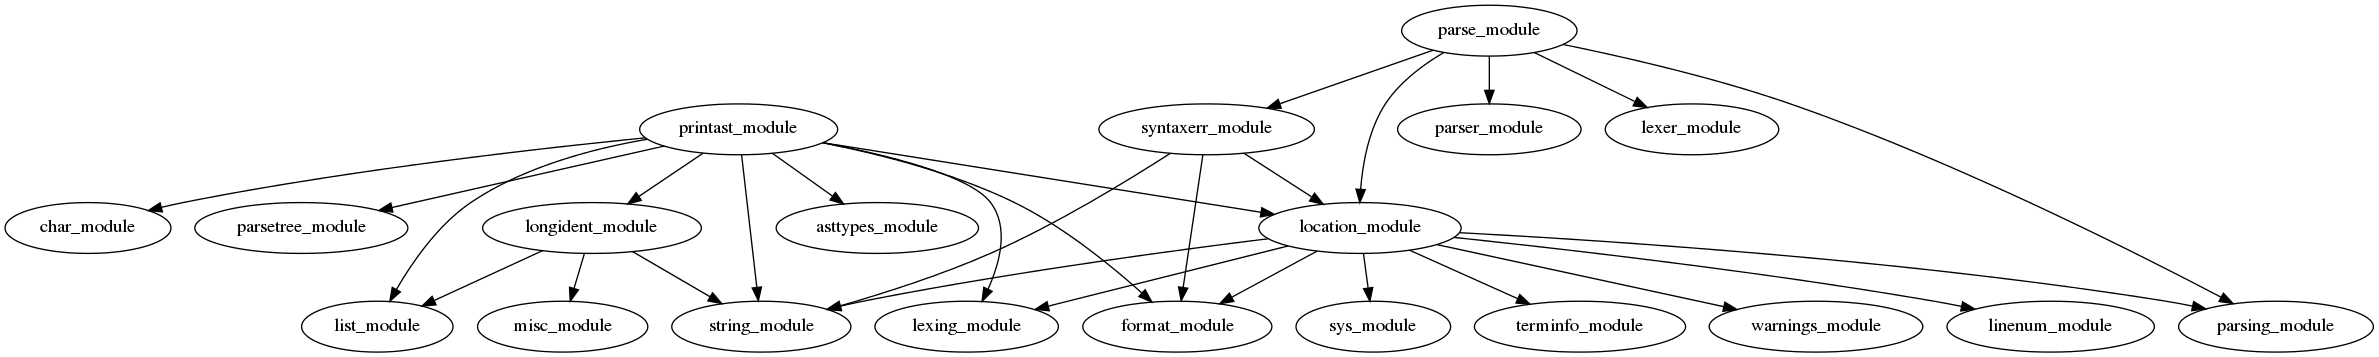
\includegraphics[scale=0.2,angle=-90]{graphics/parsing_dep.png}
  \caption{parsing depdency}
  \label{fig:parsing_dep}
\end{figure}


\begin{ocamlcode}
type constant =
    Const_int of int
  | Const_char of char
  | Const_string of string
  | Const_float of string
  | Const_int32 of int32
  | Const_int64 of int64
  | Const_nativeint of nativeint
type rec_flag = Nonrecursive | Recursive | Default
type direction_flag = Upto | Downto
type private_flag = Private | Public
type mutable_flag = Immutable | Mutable
type virtual_flag = Virtual | Concrete
type override_flag = Override | Fresh
type closed_flag = Closed | Open
type label = string
\end{ocamlcode}
\captionof{listing}{asttypes \label{asttypes}}

\newpage
\inputminted[fontsize=\scriptsize]{ocaml}{code/compiler/ast.ml}
\captionof{listing}{ocaml parsing ast}

In \textit{parsing} directory, \textit{parser.mly} defines BNF of oaml
\textit{parse} is a wrapper of \textit{parsing},
\textit{parsetree.mli}(used by ocamlyacc) defines the \textit{ast}
type. \textit{printast.ml} defines the pretty printer for ocaml ast.

It's easy to play with parsing api.

\begin{ocamlcode}
  #load ``toplevellib.cma'';;
  #directory ``+../compiler-lib'';;
  Parse.implementation (Lexing.from_string "let a =  M.(b + 3) ");;
\end{ocamlcode}

As we said before, \textit{Printtyp} pretty print the output typing
ast. \textit{typecore} implement type inference for the core language.
\textit{typemode.ml} type checking the module language.

\section{typing}

\textit{typedtree.mli} defines ast after typing,
\textit{outcometree}defined results displayed by the toplevel

These types represent messages that the toplevel displays as normal
results or errors. The real displaying is customisable using the
hooks: \textit{Toploop.print\_out\_value},
\textit{Toploop.print\_out\_type}
\textit{Toploop.print\_out\_sig\_item},
\textit{Toploop.print\_out\_phrase}


\section{Bytecomp}

When we get \textit{typedtree} output, we will compile it to byte
code.  module Lambda defines the intermediate language. module Typeopt
introduced some type-based optimizations.  module Bytegen defines
generation of bytecode from lambda terms. module Emitcode defined
generation of bytecode for \textit{.cmo} files.


\subsection{Symtable}

\begin{ocamlcode}
value get_global_value : Ident.t -> Obj.t;
\end{ocamlcode}

\subsection{Translmod}

A module which translate typedtree to lamda terms

\begin{ocamlcode}
val transl_toplevel_definition: structure -> lambda
\end{ocamlcode}

\subsection{Simplify}
A module eliminate useless Alias bindings.

\begin{ocamlcode}
  value simplify_lambda : Lambda.lambda -> Lambda.lambda;
  value is_tail_native_heuristic : ref (int -> bool);
\end{ocamlcode}

\subsection{Bytegen}
A module translate lambda terms to lists of instructions
\begin{ocamlcode}
val compile_implementation: string -> lambda -> instruction list
(* the first argument is a module name *)

val compile_phrase: lambda -> instruction list * instruction list
(* return (init_code,fun_code0 as a tuple *)
\end{ocamlcode}

\subsection{Emitcode}

\begin{ocamlcode}
val to_memory: instruction list -> instruction list ->
                    string * int * (reloc_info * int) list
        (* Arguments:
             initialization code (terminated by STOP)
             function code
           Results:
             block of relocatable bytecode
             size of this block
             relocation information *)
\end{ocamlcode}


\subsection{Meta}

A module to control the runtime system and bytecode interpreter.

It was written in C language.

\section{byterun}

Runtime

%% \chapter{Book}
%% \subsection{Developing Applications with Objective Caml}

\begin{enumerate}
  \item caveat
    \begin{enumerate}
    \item + (modulo the boundary, \emph{will not be checked})
    \item $1.0/0.0 \rightarrow \infty $
    \item $+. -. *. /. **$  mod ceil floor sqrt exp log log10 cos sin tan acos asin atan  
    \item $asin 3.14  \rightarrow nan    $
    \item \verb|char_of_int 255| $\rightarrow$ \verb|'\255'| (can not display)
    \item \verb|char_of_int int_of_char string_of_int int_of_string|
      \verb|string_of_int 2551 -> ``2551''|
    \item string (length $\le 2^{24} - 6$ )
    \item == (\textit{physical equal}) (=, != <>)


\begin{alternate}
true == true;;
- : bool = true
# 3 == 3;;
- : bool = true
# 1. == 1.;;
- : bool = false
\end{alternate}

    \item int * int * int is different from (int * int ) * int
    \item unreasonable parametric equality \verb|(=) : 'a -> 'a -> bool|
    \item recursive declaration

\begin{ocamlcode}
let rec ones = 1 :: ones;;
\end{ocamlcode}

\begin{ocamlcode}
val ones : int list =
  [1; 1; 1; 1; 1; 1; 1; 1; 1; 1; 1; 1; 1; 1; 1; 1; 1; 1; 1; 1; 1; 1; 1; 1; 1;
   1; 1; 1; 1; 1; 1; 1; 1; 1; 1; 1; 1; 1; 1; 1; 1; 1; 1; 1; 1; 1; 1; 1; 1; 1;
   1; 1; 1; 1; 1; 1; 1; 1; 1; 1; 1; 1; 1; 1; 1; 1; 1; 1; 1; 1; 1; 1; 1; 1; 1;
   1; 1; 1; 1; 1; 1; 1; 1; 1; 1; 1; 1; 1; 1; 1; 1; 1; 1; 1; 1; 1; 1; 1; 1; 1;
   1; 1; 1; 1; 1; 1; 1; 1; 1; 1; 1; 1; 1; 1; 1; 1; 1; 1; 1; 1; 1; 1; 1; 1; 1;
   1; 1; 1; 1; 1; 1; 1; 1; 1; 1; 1; 1; 1; 1; 1; 1; 1; 1; 1; 1; 1; 1; 1; 1; 1;
   1; 1; 1; 1; 1; 1; 1; 1; 1; 1; 1; 1; 1; 1; 1; 1; 1; 1; 1; 1; 1; 1; 1; 1; 1;
   1; 1; 1; 1; 1; 1; 1; 1; 1; 1; 1; 1; 1; 1; 1; 1; 1; 1; 1; 1; 1; 1; 1; 1; 1;
   1; 1; 1; 1; 1; 1; 1; 1; 1; 1; 1; 1; 1; 1; 1; 1; 1; 1; 1; 1; 1; 1; 1; 1; 1;
   1; 1; 1; 1; 1; 1; 1; 1; 1; 1; 1; 1; 1; 1; 1; 1; 1; 1; 1; 1; 1; 1; 1; 1; 1;
   1; 1; 1; 1; 1; 1; 1; 1; 1; 1; 1; 1; 1; 1; 1; 1; 1; 1; 1; 1; 1; 1; 1; 1; 1;
   1; 1; 1; 1; 1; 1; 1; 1; 1; 1; 1; 1; 1; 1; 1; 1; 1; 1; 1; 1; 1; 1; 1; 1;
   ...]
\end{ocamlcode}


\begin{ocamlcode}
 let special_size l = 
    let rec size_aux prev = function 
      |[] -> 0 
      |_ :: l1  -> if List.memq l1 prev then 1 else 1 + size_aux (l1::prev) l1 in size_aux [l]  l;;
    \end{ocamlcode}
\begin{ocamlcode}    
  val special_size : 'a list -> int = <fun>
\end{ocamlcode}

\begin{alternate}
# special_size ones;;
- : int = 1
# let rec twos = 1 :: 2 :: twos in special_size twos;;
- : int = 2
# special_size [];;
- : int = 0
\end{alternate}  
\item combine patterns \\
  p1 | .. |  pn (all name is forbidden within these patterns) 
 'a' .. 'e' 

 \begin{alternate}
let test 'a' .. 'e' = true;;
^^^^^^^^^^^^^^^^^
 \end{alternate}

\begin{ocamlcode}
Warning 8: this pattern-matching is not exhaustive.
Here is an example of a value that is not matched:
'f'
val test : char -> bool = <fun>
\end{ocamlcode}

    \item records

\begin{alternate}
type complex = {re:float;img:float};;
type complex = { re : float; img : float; }
# let add {re; img} {re; img} = 3;;
val add : complex -> complex -> int = <fun>
# let add {re; img} {re; img} = {re = re +. re; img = img +. img};;
val add : complex -> complex -> complex = <fun>
 \end{alternate}

    \item \emph{redefinition marsks the previous one, while values of the masked types
        still exist, but it now turns to be an abstract type }
    \item exception
      \begin{enumerate}
      \item \verb|Match_failure Division_by_zero Failure|
      \item exception Name of t -- monomorphic , extensible sum Type \\
        when pattern match your exception, its type should be fixed 
      \item control flow
      \end{enumerate}
    \item {\bf disagree over interface} \\
      when toplevel loads the same module (only the name is the same),
      it will check the interface is equal, this sucks since ocaml has
      flat namespace for module 
    \end{enumerate}
  \item sharing \\
    for structured values, it will be sharing , however,
    \emph{vectors of floats don't share}

\begin{alternate}
let a = Array.create 3 0.;;
val a : float array = [|0.; 0.; 0.|]
# a.(0)==a.(1);;
- : bool = false
\end{alternate}


  \item weak type variables \\

\begin{alternate}
  let b = ref []
  (* b should '_a list ref, since b is not pure, cannot be shared *)
  let a = []
  (* a : 'a list *) 
  let a = None
  (* a : 'a option *)n
  let a = Array.create 3 None
  (* '_a option array *)
# type ('a,'b) t ={ch1 : 'a list; mutable ch2 : 'b list};;
type ('a, 'b) t = { ch1 : 'a list; mutable ch2 : 'b list; }
# let v = {ch1=[];ch2=[]};;
val v : ('a, '_b) t = {ch1 = []; ch2 = []}     
\end{alternate}
 \textit{mutable sharing conflicts with polymorphism}

  \item library
    \begin{enumerate}
    \item List \\

\begin{ocamlcode}
      @ length hd tl nth rev append rev_append concat flatten
      iter map rev_map left_fold fold_right iter2 map2 rev_map2
      fold_left2 fold_right2 for_all exists for_all2 exists2 
      mem memq find filter partition assoc assq remove_assoc remove_assq
      split combine sort statble_sort fast_sort merge
    \end{ocamlcode}

\begin{alternate}    
# List.assq 3 [3,4;1,2];;
- : int = 4
# List.assq 3. [3.,4;1.,2];;
Exception: Not_found.
\end{alternate}

    \item Array \\
      \verb|Array.create_matrix creates Non-Rectangular matrices|

\begin{ocamlcode}
length get set make create init -- when you don't want to initialize
make_matrix (int->int->'a -> 'a array array) create_matrix;
append concat sub copy fill ('a array -> int -> int -> 'a -> int)
blit (Array.Labels.blit), to_list, of_list map iteri mapi fold_left
fold_right sort stable_sort fast_sort unsafe_get unsafe_set copy
\end{ocamlcode}

    \item IO \\

\begin{ocamlcode}
open_in open_out close_in close_out input_line
input : Batteries.Legacy.in_channel -> string -> int -> int -> int = <fun> 
output: Batteries.Legacy.out_channel -> string -> int -> int -> unit =<fun> 
read_line print_string print_newline print_endline
\end{ocamlcode}

    \item stack (imperative data structure actually)

\begin{ocamlcode}
exceptin Empty
create
type 'a t = { mutable c : 'a list }
(* mutable to delay initialization *)
push pop top clear copy is_empty length iter enum copy
of_enum print
module Exceptionless
  top : 'a t -> 'a option, pop
\end{ocamlcode}

    \item stream \textbf{imperative}

\begin{ocamlcode}
'a t
exception Failure
exception Error of string
from
of_list of_string of_channel iter empty peek junk count npeek
iapp icons ising lapp lcons lsing
sempty slazy dump npeek
\end{ocamlcode}

      syntax extension (for my experience, use it in shell, but not in
      tuareg toplevel)
\begin{ocamlcode}
  let concat_stream a b = [<a;b>]
\end{ocamlcode}
\begin{ocamlcode}
val concat_stream :
  'a Batteries.Stream.t -> 'a Batteries.Stream.t -> 'a Batteries.Stream.t =
\end{ocamlcode}
   expression not preceded by an \` considered to be sub-stream
   destructive pattern matching (camlp5 or extended parser can merge)
   consumed (error), failure
    \item Array List String Hashtbl Buffer Queue
    \item Sort

\begin{ocamlcode}
module X = Sort ;;
\end{ocamlcode}

\begin{ocamlcode}
module X :
  sig
    val list : ('a -> 'a -> bool) -> 'a list -> 'a list
    val array : ('a -> 'a -> bool) -> 'a array -> unit
    val merge : ('a -> 'a -> bool) -> 'a list -> 'a list -> 'a list
  end
\end{ocamlcode}

    \item Weak (vector of weak pointers) abstract type

\begin{ocamlcode}
sig
  type 'a t = 'a Weak.t
end 
\end{ocamlcode}


    \item Printf

\begin{ocamlcode}
%t -> (output->unit)
%t%s -> (output->unit)->string->unit
\end{ocamlcode}
they all should be processed at \textbf{compile time}


    \item Digest \\
      hash functions return a fingerprint of their entry (reversible) 

\begin{ocamlcode}
   val string : string -> t -- fingerprint of a string
   val file : string -> t -- fingerprint of a file 
\end{ocamlcode}

    \item Marshal estimate data size

\begin{alternate}
type external_flag = No_sharing | Closures

let size x = x |> flip Marshal.to_string [] |> flip Marshal.data_size 0;;           ;;
val size : 'a -> int = <fun>
# size 3;;
- : int = 1
# size 3.;;
- : int = 9
# size "ghsogho";;
- : int = 8
# size "ghsogho1";;
- : int = 9
# size "ghsogho1ah";;
- : int = 11
# size 111;;
- : int = 2
\end{alternate}


    \item Sys

\begin{ocamlcode}
os_type interactive word_size max_string_length
max_array_length time argv getenv command file_exists
remove rename chdir getcwd 
\end{ocamlcode}

\begin{alternate}
# float (Sys.max_string_length ) /. (2. ** 57.);;
- : float = 0.999999999999999889
\end{alternate}


    \item Arg Filename Printexc
    \item Printexc

\begin{ocamlcode}
# module P = Printexc;;
\end{ocamlcode}

\begin{ocamlcode}
module P :
  sig
    val to_string : exn -> string
    val catch : ('a -> 'b) -> 'a -> 'b
    val get_backtrace : unit -> string
    val record_backtrace : bool -> unit
    val backtrace_status : unit -> bool
    val register_printer : (exn -> string option) -> unit
    val pass : ('a -> 'b) -> 'a -> 'b
    val print : 'a BatInnerIO.output -> exn -> unit
    val print_backtrace : 'a BatInnerIO.output -> unit
  end
\end{ocamlcode}


    \item Num
    \item \verb|Arith_status|

\begin{ocamlcode}
# module X = Arith_status;;
\end{ocamlcode}
\begin{ocamlcode}
module X :
  sig
    val arith_status : unit -> unit
    val get_error_when_null_denominator : unit -> bool
    val set_error_when_null_denominator : bool -> unit
    val get_normalize_ratio : unit -> bool
    val set_normalize_ratio : bool -> unit
    val get_normalize_ratio_when_printing : unit -> bool
    val set_normalize_ratio_when_printing : bool -> unit
    val get_approx_printing : unit -> bool
    val set_approx_printing : bool -> unit
    val get_floating_precision : unit -> int
    val set_floating_precision : int -> unit
  end
\end{ocamlcode}


    \item Dynlink \\
      choice at execution time, load a new module and hide the
      code code (hot-patch)
      actually (\#load is kinda hot-patch), however to write it in programs
      \emph{more flexible} than \#load , load requires its name are fixed, and
      load will check .mli file, Dynlink \textbf{does not} do this check, while when you
      want to do X.blabla, it still checks, so still don't work, only side
      effects will work.

\begin{ocamlcode}
#direcotry "+dynlink";;
#load "dynlink.cma";;
Dynlink.loadfile "test.cmo";;
\end{ocamlcode}

    \end{enumerate}

  \item syntaxes
  \item expr

\begin{ocamlcode}
exp	::=value-path  -- value-name or module-path.value-name
 	| constant  
 	| ( expr )  
 	| begin expr end  
 	| ( expr :  typexpr )  
 	| expr ,  expr  { , expr } -- tuple
 	| constr  expr  -- constructor
 	| `tag-name  expr  -- polymorphic variant
 	| expr ::  expr  -- list 
 	| [ expr  { ; expr } ]  
 	| [| expr  { ; expr } |]  
 	| { field =  expr  { ; field =  expr } }  
 	| { expr with  field =  expr  { ; field =  expr } }  
 	| expr  { argument }+ -- application  
 	| prefix-symbol  expr  -- prefix operator
 	| expr  infix-op  expr  
 	| expr .  field  
 	| expr .  field <-  expr  -- still an expression
 	| expr .(  expr )  
 	| expr .(  expr ) <-  expr  
 	| expr .[  expr ]  
 	| expr .[  expr ] <-  expr  
 	| if expr then  expr  [ else expr ]  
 	| while expr do  expr done  
 	| for ident =  expr  ( to |  downto ) expr do  expr done  
 	| expr ;  expr  
 	| match expr with  pattern-matching  
 	| function pattern-matching  
 	| fun multiple-matching  -- multiple parameters matching
 	| try expr with  pattern-matching  
 	| let [rec] let-binding   { and let-binding } in  expr  
 	| new class-path  
 	| object class-body end  
 	| expr #  method-name  
 	| inst-var-name  
 	| inst-var-name <-  expr  
 	| ( expr :>  typexpr )  
 	| ( expr :  typexpr :>  typexpr )  
 	| {< inst-var-name =  expr  { ; inst-var-name =  expr } >}  
 	| assert expr  
 	| lazy expr  
 
argument::=expr  
 	| ~ label-name  
 	| ~ label-name :  expr  
 	| ? label-name  
 	| ? label-name :  expr  
 
pattern-matching::=
 [|] pattern [when expr]-> expr { |pattern  [when expr] ->  expr }  
 
multiple-matching::= { parameter }+  [when expr]-> expr  
 
let-binding::=pattern =  expr  
 	| value-name  { parameter }  [: typexpr] =  expr  
 
parameter::=pattern  
 	| ~ label-name  
 	| ~ ( label-name  [: typexpr] )  
 	| ~ label-name :  pattern  
 	| ? label-name  
 	| ? ( label-name  [: typexpr]  [= expr] )  
 	| ? label-name :  pattern  
 	| ? label-name : (  pattern  [: typexpr]  [= expr] )
\end{ocamlcode}        
      
\begin{alternate}
  let f ?test:(Some x ) y = x + y;;
  ^^^^^^^^^^^^^^^^^^^^^^^^^
\end{alternate}

\begin{ocamlcode}
Warning 8: this pattern-matching is not exhaustive.
Here is an example of a value that is not matched:
None
val f : ?test:int -> int -> int = <fun>
\end{ocamlcode}

  \item pattern

\begin{ocamlcode}
pattern	::=	value-name  
 	| _  
 	| constant  
 	| pattern as  value-name  
 	| ( pattern )  
 	| ( pattern :  typexpr )  
 	| pattern |  pattern  
 	| constr  pattern  
 	| `tag-name  pattern  
 	| #typeconstr-name  -- object ?
 	| pattern  { , pattern }  
 	| { field =  pattern  { ; field =  pattern } }  
 	| [ pattern  { ; pattern } ]  
 	| pattern ::  pattern  
 	| [| pattern  { ; pattern } |]  
 	| lazy pattern
\end{ocamlcode}

  \item toplevel-phrase

\begin{ocamlcode}
toplevel-input::= { toplevel-phrase } ;;  
 
toplevel-phrase::=definition  
 	| expr  
 	| #ident  directive-argument  
 
directive-argument::=epsilon
 	| string-literal  
 	| integer-literal  
 	| value-path
defition ::= let [rec] let-binding {and let-binding}
        | external value-name : typexpr = external-declartion
        | type-definition
        | exception-defition
        | class-definition
        | classtype-definition
        | module module-name {(module-name : module-type)} [:module-type] = module-expr
        | module type module-name = module-type
        | open module-path
        | include module-expr 
\end{ocamlcode}

  \item type-definition

\begin{ocamlcode}

type-definition	::= type typedef  { and typedef }  
 
typedef	::= [type-params]  typeconstr-name  [type-information]  
 
type-information::=
  [type-equation] [type-representation]{ type-constraint }  
type-equation::= = typexpr  
 
type-representation::=
          = constr-decl  { | constr-decl }  
 	| = { field-decl  { ; field-decl } }  

type-params::=	type-param  
 	| ( type-param  { , type-param } )  
 
type-param::=	' ident  
 	| + ' ident  
 	| - ' ident  
 
constr-decl::=	constr-name  
 	| constr-name of  typexpr  { * typexpr }  
 
field-decl::=	field-name :  poly-typexpr  
 	| mutable field-name :  poly-typexpr  
type-constraint	::=constraint ' ident =  typexpr
\end{ocamlcode}

\begin{alternate}
# type t;;
type t
\end{alternate}

\item  interoperating with C

  Difficutilies 
  \begin{enumerate}
  \item Machine reperesentation of data
  \item GC \\
    calling a c function from ocaml must not modify the memory in ways incompatible
    with ocaml gc.
  \item Exceptions \\
    C does not support exceptions, different mechanisms for aborting computations,
    this complicates ocaml's exception handling
  \item sharing common resources \\
    input-output. each language maintains its own input-output buffers.
  \end{enumerate}

  Communications
  \begin{enumerate}
  \item external declarations \\
    it associates a c function definition with an ocaml name, while giving the
    type of the latter.

    \begin{bluetext}
      external caml_name : type = "C_name"
      val caml_name : type
    \end{bluetext}
    both workds, but in the latter case, calls to the c function \textit{first go}
    through the general function application mechanism of ocaml. This is slightly
    less efficient, but hides the implementation of the function as a c function.
  \item external functions with more than five arguments
    \begin{bluetext}
      external caml_name : type = "C_name_bytecode" "C_name_native"
    \end{bluetext}
  \end{enumerate}

  
\end{enumerate}

\subsubsection{chap7 Development Tools}
\label{sec:chap7-devel-tools}
\begin{enumerate}

\item Command names  \\
  

  


\item chap10 Program Analysis Tool \\
  \begin{enumerate}
  \item ocamldep \\

    
    \begin{tabular}{|c|c|}
      -I & add dir \\
      -impl,-intf & \\
      -ml(i)-synonym <e> & cosider <e> as a synonym of .ml(i) extension \\
      -modules & Print module dependencies in raw form(not suitable for make) \\
      -native & generate dependencies for a pure native-code project \\
      -slash & for windows \& unix \\
    \end{tabular}

    
\begin{ocamlcode}
ocamldep -modules *.ml      
\end{ocamlcode}

\begin{ocamlcode}
ta.ml: Array Printf
tb.ml: Array Ta
\end{ocamlcode}

  \begin{ocamlcode}
ocamldep *.ml    
\end{ocamlcode}


\begin{ocamlcode}
ta.cmo:
ta.cmx:
tb.cmo: ta.cmo
tb.cmx: ta.cmx
\end{ocamlcode}

other examples

\begin{bluetext}
ocamlfind ocamldep -modules dir_top_level_util.ml > dir_top_level_util.ml.depends
ocamlfind ocamldep -pp 'camlp4of -parser pa_mikmatch_pcre.cma' -modules dir_top_level.ml > dir_top_level.ml.depends
\end{bluetext}

\item debug

  \#(un)trace command ,\#untrace\_all.
  \begin{alternate}
let verify_div a b q r = a = b * q + r ;;
val verify_div : int -> int -> int -> int -> bool = <fun>
# #trace verif_div ;;
Unbound value verif_div.
# #trace verify_div ;;
verify_div is now traced.
\end{alternate}

\begin{ocamlcode}
verify_div 11 5 2 1 ;;  
\end{ocamlcode}


\begin{ocamlcode}
verify_div <-- 11
verify_div --> <fun>
verify_div* <-- 5
verify_div* --> <fun>
verify_div** <-- 2
verify_div** --> <fun>
verify_div*** <-- 1
verify_div*** --> true
- : bool = true  
\end{ocamlcode}

\begin{bluetext}
let rec belongs_to (e:int) = function 
    | [] -> false 
    | t :: q -> (e=t) || belongs_to e q;;
    val belongs_to : int -> int list -> bool = <fun>
# #trace belongs_to;;
belongs_to is now traced.
# belongs_to 4 [3;5;7;4];;
belongs_to <-- 4
belongs_to --> <fun>
belongs_to* <-- [3; 5; 7; 4]
belongs_to <-- 4
belongs_to --> <fun>
belongs_to* <-- [5; 7; 4]
belongs_to <-- 4
belongs_to --> <fun>
belongs_to* <-- [7; 4]
belongs_to <-- 4
belongs_to --> <fun>
belongs_to* <-- [4]
belongs_to* --> true
belongs_to* --> true
belongs_to* --> true
belongs_to* --> true
- : bool = true
\end{bluetext}

\begin{bluetext}
# let rec belongs to (e : int) = function
[] -> false
| t :: q -> belongs to e q || (e = t) ; ;
val belongs_to : int -> int list -> bool = <fun> # #trace belongs to ;;
belongs_to is now traced.
# belongs to 3 [3;5;7] ;;
belongs_to <-- 3
belongs_to --> <fun>
belongs_to* <-- [3; 5; 7]
belongs_to <-- 3
belongs_to --> <fun>
belongs_to* <-- [5; 7]
belongs_to <-- 3
belongs_to --> <fun>
belongs_to* <-- [7]
belongs_to <-- 3
belongs_to --> <fun>
belongs_to* <-- []
belongs_to* --> false
belongs_to* --> false
belongs_to* --> false
belongs_to* --> true
- : bool = true  
\end{bluetext}


Trace providing a mechanism for the efficiency analysis of recursive functions, not that friendly, however, no idented output.
To make things worse, trace \textit{does not show the value corresponding to an argument of a parameterized type}. The toploop can show
only monomorphic types.

Moreover, it only keeps the inferred types of
\textit{global declarations}. Therefore after compilation of the
expression, the toplevel in fact \textit{no longer } processes any
furthuer type information about the expression.

Only global type declarations are kept in the environment of the
toplevel loop, \textit{local functions} can not be traced for the same reasons
as above
\begin{bluetext}
let rec belongs_to e = function 
    | [] -> false 
    | t :: q -> (e=t) || belongs_to e q;;
    val belongs_to : 'a -> 'a list -> bool = <fun>
# belongs_to 4 [3;5;7;4];;
- : bool = true
# #trace belongs_to;;
belongs_to is now traced.
# belongs_to 4 [3;5;7;4];;
belongs_to <-- <poly>
belongs_to --> <fun>
belongs_to* <-- [<poly>; <poly>; <poly>; <poly>]
belongs_to <-- <poly>
belongs_to --> <fun>
belongs_to* <-- [<poly>; <poly>; <poly>]
belongs_to <-- <poly>
belongs_to --> <fun>
belongs_to* <-- [<poly>; <poly>]
belongs_to <-- <poly>
belongs_to --> <fun>
belongs_to* <-- [<poly>]
belongs_to* --> true
belongs_to* --> true
belongs_to* --> true
belongs_to* --> true
- : bool = true
\end{bluetext}

\item ocamldbg

  The \textit{-g} option produces a \textit{.cmo} file with the
  debugging information. (bytecode only)
  \end{enumerate}
\end{enumerate}
%%% Local Variables: 
%%% mode: latex
%%% TeX-master: "../master"
%%% End: 





%% \subsection{Ocaml for scientists}
\label{sec:ocaml-scientists}
\begin{itemize}
\item caveat
  \begin{itemize}
  \item string char
    \verb|'a' = '\097'|
    \verb|"Hello world".[4]|

\begin{alternate}
  [|1;2;3|].(1)
  2 
\end{alternate}

  \item objects

\begin{redcode}

(* it's a type class type *)
class type number = object
  method im:float
  method re:float 
end
\end{redcode}

\begin{redcode}
class complex x y = object 
    val x = x
    val y = y
    method re:float = x
    method im:float = y
end ;;
let b : number = new complex 3. 4.
\end{redcode}

\begin{alternate}
# let b = new complex 3. 4.;;
val b : complex = <obj>
# let b : number = new complex 3. 4.;;
val b : number = <obj>
 \end{alternate}

\begin{redcode} 
# let make_z x y = object
    val x : float = x
    val y : float = y
    method re = x
    method im = y
    end;;
  \end{redcode}
\begin{bluecode}  
val make_z : float -> float -> < im : float; re : float > = <fun>
\end{bluecode}

class type is kinda interface

  
\begin{redcode}
# let abs_number (z:number) = 
       let sqr x = x *. x in 
       sqrt (sqr z#re +. sqr z#im);;
     \end{redcode}
     
think class as a module 


  \item asr (arith) (**) lsr
  \item elements

\begin{alternate}
  [1;2;3;4] |> Set.of_list |> Set.elements;;
  - : int list = [1; 2; 3; 4]
\end{alternate}


  \end{itemize}
\item convention
\item GMP (GNU library for arbitrary precision arithmetic)

\begin{bluecode}
module type INT_RANGE = sig
type t
val make : int -> int -> t
end 
\end{bluecode}


\item Hashtbl(create, Make)
  Hahsing is another form of structural comparison and should not be applied
  {\bf to abstract types}
  \emph{Semantically equivalent sets are likely to produce different hashes}
  notice \textit{Map.empty is polymorphic, Hashtbl.empty is monomorphic}
\end{itemize}


%%% Local Variables: 
%%% mode: LaTex
%%% TeX-master: "../master"
%%% End: 

%% 
\subsection{caltech ocaml book}


  
polymorphic variants
  \begin{enumerate}
  \item simple example

\begin{alternate}
let string_of_number = function `Integer i -> i;;
val string_of_number : [< `Integer of 'a ] -> 'a = <fun>
\end{alternate}
    
\begin{ocamlcode}  
# let string_of_number = function
    |`Integer i -> i
    |_ -> invalid_arg "string_of_number";;
  \end{ocamlcode}
\begin{ocamlcode}  
  val string_of_number : [> `Integer of 'a ] -> 'a = <fun>
\end{ocamlcode}  

\begin{ocamlcode}
let test0 = function 
  |`Int i -> i

let test1 = function 
  |`Int i -> i 
  | _ -> invalid_arg "invalid arg in test1"

let test2 = function 
  |x -> test0 x

let test3 = function 
  |x -> test1 x

(* let test4 : [> `Real of 'a | `Int of 'a ] -> 'a = function 
   |`Real x -> x *)
   | x -> test0 (x:> [< `Int of 'a])  *)

let test5 = function 
  |`Real x -> x 
  | x -> test1 x 
  
\end{ocamlcode}

\begin{ocamlcode}
val test0 : [< `Int of 'a ] -> 'a = <fun>
val test1 : [> `Int of 'a ] -> 'a = <fun>
val test2 : [< `Int of 'a ] -> 'a = <fun>
val test3 : [> `Int of 'a ] -> 'a = <fun>
val test5 : [> `Int of 'a | `Real of 'a ] -> 'a = <fun>
\end{ocamlcode}

for open union, it's easy to reuse, but \textbf{unsafe},
for closed union, hard to use, since the type checker is
conservative


\begin{alternate}

test1 `Test;;
Exception: Invalid_argument "invalid arg in test1".

test0 `Test;;
Characters 6-11:
  test0 `Test;;
        ^^^^^
Error: This expression has type [> `Test ]
       but an expression was expected of type [< `Int of 'a ]
       The second variant type does not allow tag(s) `Test
\end{alternate}
     






  \item \textbf{define polymorphic variant type }

\begin{alternate}
type number = [> `Integer of int | `Real of float ];;
       ^^^^^^^^^^^^^^^^^^^^^^^^^^^^^^^^^^^^^^^^^^^^^^
Error: A type variable is unbound in this type declaration.
In type [> `Integer of int | `Real of float ] as 'a
the variable 'a is unbound

type 'a number = 'a constraint 'a = [>`Integer of int | `Real of float]

let zero : 'a number = `Zero;;
val zero : [> `Integer of int | `Real of float | `Zero ] number = `Zero


type number = [< `Integer of int | `Real of float ];;
       ^^^^^^^^^^^^^^^^^^^^^^^^^^^^^^^^^^^^^^^^^^^^^^
Error: A type variable is unbound in this type declaration.
In type [< `Integer of int | `Real of float ] as 'a
the variable 'a is unbound
# type number = [ `Integer of int | `Real of float ];;
type number = [ `Integer of int | `Real of float ]


\end{alternate}

  \item \textbf{sub-typing for polymorphic variants}

\begin{ocamlcode}
  [`A] :> [`A | `B]
\end{ocamlcode}  
since you know how to handle A and B, then you know how to handle A

\begin{alternate}
let f x = (x:[`A] :> [`A | `B ]);;
val f : [ `A ] -> [ `A | `B ] = <fun>
\end{alternate}

ocaml does has width and depth subtyping
if t1 :> t1' and t2 :> t2' then (t1,t2) :> (t1',t2')

\begin{alternate}
let f x = (x:[`A] * [`B] :> [`A|`C] * [`B | `D]);; 
val f : [ `A ] * [ `B ] -> [ `A | `C ] * [ `B | `D ] = <fun>


let f x = (x : [ `A | `B ] -> [ `C ] :> [ `A ] -> [ `C | `D ]);;
val f : ([ `A | `B ] -> [ `C ]) -> [ `A ] -> [ `C | `D ] = <fun>
\end{alternate}

  \item variance notation \\
    if you don't write the + and -, ocaml will \textbf{infer} them for you ,
    but when you write abstract type in module type signatures, it makes sense.
    variance annotations \textbf{allow you to expose the subtyping properties} of your type
    in an interface, without exposing the representation.

\begin{ocamlcode}
type (+'a, +'b) t = 'a * 'b
type (-'a,+'b) t = 'a -> 'b 
module M : sig
  type (+'a,'+b) t
end = struct
  type ('a,'b) t = 'a * 'b 
end
\end{ocamlcode}
ocaml did the check when you define it, so you can not define it arbitrarily

  \item \textbf{co-variant} helps polymorphism

\begin{alternate}
module M : sig
    type +'a t
    val embed : 'a -> 'a t
  end = struct
    type 'a t = 'a
    let embed x = x
end ;;
M.embed []  ;;
- : 'a list M.t = <abstr>
\end{alternate}


  \item example

\begin{alternate}
type suit = [ `Club | `Diamond | `Heart | `Spade ]
  
let winner = function `Heart -> true | #suit -> false;;
val winner : [< suit ] -> bool = <fun>
let winner2 = function `Unknown -> true |#suit -> false;;
val winner2 : [< `Club | `Diamond | `Heart | `Spade | `Unknown ] -> bool =
  <fun>

(* the variant tag does not belong to a particular type *)

let winner3 : (suit -> bool) = function `Unknown -> true | #suit -> false;;
                                          ^^^^^^^^
Warning 11: this match case is unused.
val winner3 : suit -> bool = <fun>

\end{alternate}

  \end{enumerate}
%%% Local Variables: 
%%% mode: latex
%%% TeX-master: "../master"
%%% End: 

%% \subsection{The functional approach to programming}
\label{sec:funct-appr-progr}

%%% Local Variables: 
%%% mode: latex
%%% TeX-master: "../master"
%%% End: 

%% \subsection{practical ocaml}
\label{sec:practical-ocaml}


\begin{enumerate}
\item chap30 \\

  \begin{bluetext}
external functions_can_be_defined: unit -> unit = "int_c_code"     
  \end{bluetext}
\end{enumerate}

%%% Local Variables: 
%%% mode: latex
%%% TeX-master: "../master"
%%% End: 

%% \subsection{hol-light}
\label{sec:hol-light}
\begin{itemize}
\item \href{http://code.google.com/p/hol-light/}{hol-light} 
\end{itemize}

%%% Local Variables: 
%%% mode: latex
%%% TeX-master: "../master"
%%% End: 

%% \section{UNIX system programming in ocaml}
\label{sec:unix-syst-progr}

\subsection{chap1}
\label{sec:chap1}

\begin{enumerate}
\item Modules Sys and Unix \\
  \textbf{Sys} containts those functions common to Unix and Windows.
  \textbf{Unix} contains everything specific to Unix.

  The \textit{Sys} and \textit{Unix} modules can override certain
  functions of the \textit{Pervasives} module
  \begin{alternate}
Unix.stdin;;
- : Batteries.Unix.file_descr = <abstr>
Pervasives.stdin;;
- : in_channel = <abstr>
\end{alternate}

\begin{ocamlcode}
  <prog.{native,byte}> : use_unix
  ocamlmktop -o ocamlunix unix.cma
\end{ocamlcode}

When running a program from a shell, the shell passes \textbf{arguments} and
\textbf{environment} to the program. When a program terminates
prematurely because \textit{an exception was raised but not caught}, it makes
an implicit call to \textit{exit 2}. For \textit{at\_exit}, the last
function to be registered is called first, and it can not be
unregistered. However, we can walk around it using global variables.

\begin{ocamlcode}
  Sys.argv, Sys.getenv , Unix.environment, 
  Pervasives.exit, Pervasives.at_exit, Unix.handle_unix_error
\end{ocamlcode}
\begin{alternate}
Sys.argv;;
\end{alternate}
\begin{ocamlcode}
- : string array =
[|"/Users/bob/SourceCode/ML/godi/bin/ocaml"; "dynlink.cma";
"camlp4of.cma"; "-warn-error"; "+a-4-6-27..29"|]
\end{ocamlcode}
\begin{alternate}
  Unix.environment ();;
\end{alternate}
\begin{ocamlcode}
- : string array =
[|"TERM=dumb"; "SHELL=/bin/bash";
  "TMPDIR=/var/folders/R4/R4awSXDIH6GpuuMmaVeCzU+++TI/-Tmp-/";
  "LIBRARY_PATH=/opt/local/lib/";
  "EMACSDATA=/Applications/Aquamacs.app/Contents/Resources/etc";
  "Apple_PubSub_Socket_Render=/tmp/launch-mcHkKo/Render";
  "EMACSPATH=/Applications/Aquamacs.app/Contents/MacOS/bin";
  "INCLUDE_PATH=/opt/local/include/"; "EMACS=t"; "USER=bob";
  "LD_LIBRARY_PATH=/opt/local/lib/"; "COMMAND_MODE=unix2003"; "TERMCAP=";
  "SSH_AUTH_SOCK=/tmp/launch-g9AcyQ/Listeners";
  "__CF_USER_TEXT_ENCODING=0x1F5:0:0"; "COLUMNS=68";
  "PATH=/opt/local/sbin:/usr/local/smlnj/bin:/usr/local/lib:/Applications/MATLAB_R2010b.app/bin:~/SourceCode/scala/scala-2.9.0.final/bin:/Users/bob/SourceCode/scripts:~/lib/emacs/customize:/usr/local/git/bin:/Users/bob/Racket/bin:/Users/bob/.cabal/bin:/Users/bob/SourceCode/ML/godi/bin:/Users/bob/SourceCode/ML/godi/sbin:/usr/texbin/:/bin:/usr/bin:/opt/local/bin/:/usr/local/lib/:/usr/local/bin/";
  "_=/usr/local/bin/ledit"; "C_INCLUDE_PATH=/opt/local/include/";
  "PWD=/Users/bob/SourceCode/Notes/ocaml-book";
  "TEXINPUTS=.:/Applications/Aquamacs.app/Contents/Resources/lisp/aquamacs/edit-modes/auctex/latex:";
  "EMACSLOADPATH=/Applications/Aquamacs.app/Contents/Resources/lisp:/Applications/Aquamacs.app/Contents/Resources/leim";
  "SHLVL=3"; "HOME=/Users/bob"; "LOGNAME=bob";
  "CAMLP4_EXAMPLE=/Users/bob/SourceCode/ML/godi/build/distfiles/ocaml-3.12.0/camlp4/examples/";
  "DISPLAY=/tmp/launch-sXEeNT/org.x:0"; "INSIDE_EMACS=23.3.50.1,comint";
  "EMACSDOC=/Applications/Aquamacs.app/Contents/Resources/etc";
  "SECURITYSESSIONID=616cd3"|]
\end{ocamlcode}

\item ERROR handling \\
  \begin{bluetext}
    exception Unix_error of error * string * string
    type error = E2BIG | ... |EUNKNOWERR of int 
  \end{bluetext}
  The second arg  of \textit{Unix\_error} is the name of the system
  call that raised the error, the third, if possible, identifies the
  object on which the error occured (i.e. file name).
  \textit{Unix.handle\_unix\_error}, if this raises the exception
  \textit{Unix\_error}, displays the message, and \textit{exit 2}


  \begin{ocamlcode}
let handle_unix_error2 f arg = let open Unix in 
  try
     f arg
  with Unix_error(err, fun_name, arg) ->
  prerr_string Sys.argv.(0);
  prerr_string ": \"";
  prerr_string fun_name;
  prerr_string "\" failed";
  if String.length arg > 0 then begin
     prerr_string " on \"";
     prerr_string arg;
     prerr_string "\"" end;
     prerr_string ": ";
     prerr_endline (error_message err);
     exit 2;;  
   \end{ocamlcode}
   
   \begin{bluetext}
val handle_unix_error2 : ('a -> 'b) -> 'a -> 'b = <fun>     
\end{bluetext}

\begin{bluetext}
  let rec restart_on_EINTR f x =
  try f x with Unix_error (EINTR, _, _) -> restart_on_EINTR f x  
\end{bluetext}

\begin{alternate}
finally;;
- : (unit -> unit) -> ('a -> 'b) -> 'a -> 'b = <fun>
finally (fun _ -> print_endline "finally") (fun _ -> failwith "haha") ();;
\end{alternate}
\begin{ocamlcode}
finally
Exception: Failure "haha".
\end{ocamlcode}

In case the program fails, i.e. raises an exception, \textit{the finalizer is
run and the exception  ex is raised again}. If \textbf{both} the main function
and the finalizer fail, the finalizer's exception is raised.
\end{enumerate}

\subsection{chap2}
\label{sec:chap2}

\begin{enumerate}
\item Files \\
  \textbf{File} covers \textit{standard files, directories, symbolic
    links, special files(devices), named pipes, sockets}
\item \textbf{Filename}  module \\
  makes filename cross platform
  \begin{bluetext}
    val current_dir_name : string
    val parent_dir_name : string
    val dir_sep : string
    val concat : string -> string -> string
    val is_relative : string -> bool
    val is_implicit : string -> bool
    val check_suffix : string -> string -> bool
    val chop_suffix : string -> string -> string
    val chop_extension : string -> string
    val basename : string -> string
    val dirname : string -> string
    val temp_file : ?temp_dir:string -> string -> string -> string
    val open_temp_file :
      ?mode:open_flag list ->
      ?temp_dir:string -> string -> string -> string * out_channel
    val temp_dir_name : string
    val quote : string -> string
  \end{bluetext}

  non-directory files can have \textbf{many parents}(we say that they have many
  \textbf{hard links}). There are also \textit{symbolic links} which
  can be seen as \textit{non-directory} files containing a path, conceptually,
  this path can be obtained by reading the contents of the symbolic
  link like an ordinary file. Whenever a symbolic link occurs in the
  \textbf{middle} of  a path, we have to follow its path
  transparently.
  \begin{bluetext}
    p/s/q -> l/q (l is absolute)
    p/s/q -> p/l/q (l is relative)
  \end{bluetext}
  \begin{bluetext}
    Sys.getcwd, Sys.chdir, Unix.chroot
  \end{bluetext}
  \textit{Unix.chroot p} makes the node p, which should be a
  directory, the root of the \textit{restricted} view of the
  hierarchy. Absolute paths are then interpreted according to this new
  root p (and .. at the new root is itself).
  Due to hard links, a file can have many different names.

\begin{ocamlcode}
Unix.(link, unlink,symlink,rename);;
\end{ocamlcode}
\begin{ocamlcode}
- : (string -> string -> unit) * (string -> unit) *
    (string -> string -> unit) * (string -> string -> unit)    
  \end{ocamlcode}
  
  \textit{unlink f} is like \textit{rm -f f}, \textit{link f1 f2} is
  like \textit{ln f1 f2}, \textit{symlink f1 f2} is like \textit{ln -s
  f1 f2}, rename f1 f2 is like \textit{mv f1 f2}

  A file descriptor represents a pointer to a file along with other
  information like the current read/write position in the file, the
  access rights, etc. \textbf{file\_descr}

  \begin{ocamlcode}
    Unix.(stdin,stdout,stderr);;
  \end{ocamlcode}
  
  \begin{ocamlcode}
  - : Batteries.Unix.file_descr * Batteries.Unix.file_descr *
    Batteries.Unix.file_descr    
  \end{ocamlcode}
  without redirections, the three descriptors refer to the terminal.
  \begin{bluetext}
    cmd > f ; cmd 2 > f
  \end{bluetext}
\item Meta attributes, types and permissions \\


  \begin{alternate}
Unix.(stat,lstat,fstat);;
  \end{alternate}
\begin{ocamlcode}  
  (string -> Batteries.Unix.stats) *
  (string -> Batteries.Unix.stats) *
  (Batteries.Unix.file_descr -> Batteries.Unix.stats)    
\end{ocamlcode}
  \textit{lstat} returns information about the symbolic link itself,
  while \textit{stat} returns information about the file that link
  points to.
  \begin{alternate}
Unix.(lstat &&& stat) "/usr/bin/al";;    
  \end{alternate}
  \begin{ocamlcode}
({Batteries.Unix.st_dev = 234881026; Batteries.Unix.st_ino = 843893;
  Batteries.Unix.st_kind = Batteries.Unix.S_LNK; (* link *)
  Batteries.Unix.st_perm = 493; Batteries.Unix.st_nlink = 1;
  Batteries.Unix.st_uid = 0; Batteries.Unix.st_gid = 0;
  Batteries.Unix.st_rdev = 0; Batteries.Unix.st_size = 46;
  (* pretty  small as a link *)
  Batteries.Unix.st_atime = 1273804908.;
  Batteries.Unix.st_mtime = 1273804908.;
  Batteries.Unix.st_ctime = 1273804908.},

 {Batteries.Unix.st_dev = 234881026; Batteries.Unix.st_ino = 840746;
  Batteries.Unix.st_kind = Batteries.Unix.S_REG; (*  regular file *)
  Batteries.Unix.st_perm = 493; Batteries.Unix.st_nlink = 1;
  Batteries.Unix.st_uid = 0; Batteries.Unix.st_gid = 80;
  Batteries.Unix.st_rdev = 0; Batteries.Unix.st_size = 163;
  (* maybe bigger *)
  Batteries.Unix.st_atime = 1323997427.;
  Batteries.Unix.st_mtime = 1271968805.;
  Batteries.Unix.st_ctime = 1273804911.})    
\end{ocamlcode}

  A file is uniquely identified by the pair made of its device
  number(typically the disk partition where it is located)
  \textit{st\_dev} and its inode number \textit{st\_ino}

  All the users and groups on the machine are usually described in the
  \textit{/etc/passwd, /etc/groups} files.
  \begin{bluetext}
    st_uid
    st_gid
    getpwnam, getgrnam, (by name, get passwd_entry, group_entry)
    getpwuid, getgrgid (by id)
    getlogin, getgroups
    chown, fchown
  \end{bluetext}

  \begin{ocamlcode}
Unix.getlogin () |> Unix.getpwnam;;    
\end{ocamlcode}

\begin{ocamlcode}
{Batteries.Unix.pw_name = "bob"; Batteries.Unix.pw_passwd = "********";
 Batteries.Unix.pw_uid = 501; Batteries.Unix.pw_gid = 20;
 Batteries.Unix.pw_gecos = "bobzhang"; Batteries.Unix.pw_dir = "/Users/bob";
 Batteries.Unix.pw_shell = "/bin/bash"}

\end{ocamlcode}

for access rights, executable, writable, readable by the user owner,
group owner, other users. For a directory, the executable permission
means the right to enter it, and read permission the right to list its
contents. The special bits do not have meaning unless the \textbf{x}
bit is set. The bit \textit{t} allows sub-directories to inherit the
permissions of the parent directory. On a directory, the bit
\textit{s} allows the use of the directory's \textit{uid} or
\textit{gid} rather than the user's to create directories. For an
executable file, the bit \textit{s} allows the chaning at executation
time of the user's effective identity or group with the system calls
\textit{setuid} and \textit{setgid}

\begin{alternate}
Unix.(setuid, getuid);;
- : (int -> unit) * (unit -> int) = (<fun>, <fun>)  
\end{alternate}

\item operations on directries \\
  only the kernel can write in directories(when files are
  created). Opening a directory in write mode is \textit{prohibited}.

  \begin{alternate}
Unix.(opendir,readdir,rewinddir,closedir);;    
\end{alternate}

\begin{ocamlcode}
- : (string -> Batteries.Unix.dir_handle) *
    (Batteries.Unix.dir_handle -> string) *
    (Batteries.Unix.dir_handle -> unit) * (Batteries.Unix.dir_handle -> unit)  
  \end{ocamlcode}

  \textit{rewinddir} repositions the descriptor at the \textbf{beginning} of
  the directory.

  \begin{ocamlcode}
    mkdir, rmdir
  \end{ocamlcode}
  We can only remove a directory that is \textbf{already empty}. It is
  thus necessary to first recursively empty the contents of the
  directory and then remove the directory.

  \begin{ocamlcode}
exception Hidden of exn 
(** add a tag to exn *)
let hide_exn f x = try f x with exn -> raise (Hidden exn)
(** strip the tag of exn *)
let reveal_exn f x = try f x with Hidden exn -> raise exn 
\end{ocamlcode}
\item  File manipulation \\

  \begin{alternate}
Unix.openfile;;    
\end{alternate}

\begin{ocamlcode}
- : string ->
    Batteries.Unix.open_flag list ->
    Batteries.Unix.file_perm -> Batteries.Unix.file_descr
  \end{ocamlcode}
  Most programs use \textit{0o666} means \textit{rw-rw-rw-}. with the default
  creation mask of \textit{0o022}, the file is thus created with the permission
  \textit{rw-r--r--}. With a more lenient mask of 0o002, the file is
  created with the permissions \textit{rw-rw-r--}. The third argument
  can be anything as \textit{O\_CREATE} is not specified.
  And to write to an empty file without caring any previous content,
  we use
  \begin{ocamlcode}
    Unix.openfile filename [O_WRONLY; O_TRUNC; O_CREAT] 0o666
  \end{ocamlcode}
  If the file is scripts, we create it with execution permission:
  \begin{ocamlcode}
    Unix.openfile filename [O_WRONLY; O_TRUNC; O_CREAT] 0o777
  \end{ocamlcode}
  If we want it to be confidential,
  \begin{ocamlcode}
    Unix.openfile filename [O_WRONLY; O_TRUNC; O_CREAT] 0o600
  \end{ocamlcode}
  The \textit{O\_NONBLOCK} flag guarantees that if the file is a named pipe or a
  special file then the file opening and subsequent reads and writes
  wil be non-blocking. The \textit{O\_NOCTYY} flag guarantees that if
  the file is a control terminal, it won't become the controlling
  terminal of the calling process.

  \begin{alternate}
    Unix.(read,single_write);;
  \end{alternate}
  \begin{ocamlcode}
  - : (Batteries.Unix.file_descr -> string -> int -> int -> int) *
    (Batteries.Unix.file_descr -> string -> int -> int -> int)
  \end{ocamlcode}    
  The \textit{string} hold the read bytes or the bytes to write. The 3rd
  argument is the start, the forth is the number.

  For writes, the number of bytes actually written is usually the
  number of bytes requested, with two exceptions
  (i) not possible to write (i.e. disk is full) (ii) the descript is a
  pipe or a socket open in non-blocking mode(async) (iii) due to
  OCaml, too large.

  The reason for (iii) is that internally OCaml uses auxiliary buffer
  whose size is bounded by a maximal value.

  OCaml also provides \textit{Unix.write} which iterates the writes
  until all the data is written or an error occurs. The problem is
  that in case of error there's no way to know the number of bytes
  that were \textit{actually written}. \textit{single\_write}
  preserves the atomicity of writes.

  For reads, when the current position is at the end of file, read
  returns zero. The convention \textit{zero equals end of file} also
  holds for special files, \textit{i.e. pipes and sockets}. For
  example, read on a terminal returns zero if we issue a
  \textit{Ctrl-D} on the input.

  But you may consider the blocking-mode in case.

  \begin{ocamlcode}
    Unix.close : file_descr -> unit 
  \end{ocamlcode}
  In contrast to Pervasives' channels, a file descriptor does not need
  to be closed to ensure that all pending writes have been performed
  as write requests are \textit{immediately} transmitted to the
  kernel. On the other hand, the number of descriptors allocated by a
  process is limited by the kernel(several hundreds to thousands).


  \begin{ocamlcode}
let buffer_size = 8192 
let buffer = String.create buffer_size 

(** this is unsatisfactory, if we copy an executable file, we would
like the copy to be also executable. *)
let file_copy input output = Unix.(
  let fd_in = openfile input [O_RDONLY] 0 in 
  let fd_out = openfile output [O_WRONLY; O_CREAT; O_TRUNC] 0o666 in 
  let rec copy_loop () = match read fd_in buffer 0 buffer_size with 
    |0 -> ()
    |r -> write fd_out buffer 0 r |> ignore; copy_loop () in 
  copy_loop ();
  close fd_in ; 
  close fd_out 
)


let copy () = 
  if Array.length Sys.argv = 3 then begin 
    file_copy Sys.argv.(1) Sys.argv.(2)
  end 
  else begin 
    prerr_endline 
      ("Usage: " ^ Sys.argv.(0) ^ "<input_file> <output_file>"); 
    exit 1 
  end 

let _  = Unix.handle_unix_error copy () 
\end{ocamlcode}

\begin{bluetext}
ocamlbuild find.byte -- find.ml find.xxxx    
\end{bluetext}

\begin{alternate}
ocamlbuild find.byte -- find.mlx find.xxxx
_build/find.byte: "open" failed on "find.mlx": No such file or directory
\end{alternate}
\item  system call \\
  For a system call, even if it does very little work, cost dearly --
  much more than a normal function call. So we need buffer to reduce
  the number of system call. For ocaml, the \textit{Pervasives} module
  adds another layer \textit{in\_channel, out\_channel}.

\item positioning and operations specific to certain file types

  \begin{alternate}
Unix.lseek;;
- : Batteries.Unix.file_descr -> int -> Batteries.Unix.seek_command -> int =
\end{alternate}

  File descriptors provide a uniform and media-independent interface
  for data communicatioin. However this uniformity breaks when we need
  to access all the features provided by a given media.

  For normal files, specific API
  \begin{ocamlcode}
Unix.(truncate,ftruncate);;
- : (string -> int -> unit) * (Batteries.Unix.file_descr -> int -> unit) =
\end{ocamlcode}
For symbolic links
\begin{ocamlcode}
Unix.(symlink, readlink);;
- : (string -> string -> unit) * (string -> string) = (<fun>, <fun>)  
\end{ocamlcode}

special files
\begin{enumerate}
\item /dev/null  black hole. (useful for ignoring the result)
\item /dev/tty* control terminals
\item /dev/pty* pseudo-terminals
\item /dev/hd* disks
\item /proc Under linux, system parameters organized as a file system.
\end{enumerate}

many special files ignore \textit{lseek}
\item terminals \\

  \begin{alternate}
Unix.(tcgetattr, tcsetattr);;
\end{alternate}
\begin{ocamlcode}
(Batteries.Unix.file_descr -> Batteries.Unix.terminal_io) *
(Batteries.Unix.file_descr ->
     Batteries.Unix.setattr_when -> Batteries.Unix.terminal_io -> unit)
\end{ocamlcode}
  
  \begin{alternate}
Unix.(tcgetattr stdout);;    
\end{alternate}

\begin{ocamlcode}
{Batteries.Unix.c_ignbrk = false; Batteries.Unix.c_brkint = true;
 Batteries.Unix.c_ignpar = false; Batteries.Unix.c_parmrk = false;
 Batteries.Unix.c_inpck = false; Batteries.Unix.c_istrip = false;
 Batteries.Unix.c_inlcr = false; Batteries.Unix.c_igncr = false;
 Batteries.Unix.c_icrnl = true; Batteries.Unix.c_ixon = false;
 Batteries.Unix.c_ixoff = false; Batteries.Unix.c_opost = true;
 Batteries.Unix.c_obaud = 9600; Batteries.Unix.c_ibaud = 9600;
 Batteries.Unix.c_csize = 8; Batteries.Unix.c_cstopb = 1;
 Batteries.Unix.c_cread = true; Batteries.Unix.c_parenb = false;
 Batteries.Unix.c_parodd = false; Batteries.Unix.c_hupcl = true;
 Batteries.Unix.c_clocal = false; Batteries.Unix.c_isig = false;
 Batteries.Unix.c_icanon = false; Batteries.Unix.c_noflsh = false;
 Batteries.Unix.c_echo = false; Batteries.Unix.c_echoe = true;
 Batteries.Unix.c_echok = false; Batteries.Unix.c_echonl = false;
 Batteries.Unix.c_vintr = '\003'; Batteries.Unix.c_vquit = '\028';
 Batteries.Unix.c_verase = '\255'; Batteries.Unix.c_vkill = '\255';
 Batteries.Unix.c_veof = '\004'; Batteries.Unix.c_veol = '\255';
 Batteries.Unix.c_vmin = 1; Batteries.Unix.c_vtime = 0;
 Batteries.Unix.c_vstart = '\017'; Batteries.Unix.c_vstop = '\019'}  
\end{ocamlcode}

it seems that ledit will change your input, and you can not get
\textit{Unix.(tcgetattr stdin)} work.

The code below works in real terminal, but does not work in
pseudo-terminals(like Emacs )

\begin{ocamlcode}
let read_passwd message = Unix.(
match 
   try 
    let default = tcgetattr stdin in 
    let silent = {default with c_echo = false; c_echoe = false ; 
                  c_echok = false; c_echonl = false ; } in 
     Some (default, silent)
   with _ -> None 
with
 |None -> Legacy.input_line Pervasives.stdin 
 |Some (default, silent) -> 
   print_string message ; 
   Legacy.flush Pervasives.stdout ; 
   tcsetattr stdin TCSANOW silent ; 
   try 
     let s = Legacy.input_line Pervasives.stdin in 
     tcsetattr stdin TCSANOW default; s 
   with x ->      tcsetattr stdin TCSANOW default; raise x 
    
);;
\end{ocamlcode}
 Sometimes a program needs to start another and connect its standard
 input to a terminal (or pseudo-terminal). To achieve that, we must
 manually look among the pseudo-terminals(/dev/tty[a-z][a-f0-9]) and
 find one that is not already open. We can open this file and start
 the program with this file on its standard input.

 The function \textit{tcsendbreak} sends an interrupt to the
 peripheral. The second argument is the duration of the interrupt.


 \begin{bluetext}
   tcdrain, tcflush, tcflow, setsid
 \end{bluetext}

\item locks on files
  \begin{bluetext}
Unix.lockf;;
- : Batteries.Unix.file_descr -> Batteries.Unix.lock_command -> int -> unit =    
\end{bluetext}

ocaml-expect
\begin{alternate}
let p = X.spawn "ocaml" [||];;
val p : X.t = <abstr>
X.expect p ~fmatches:[(fun s -> Some s)] [] "";;
- : string = "        Objective Caml version 3.12.1"
X.send p "3;;\n";;
- : unit = ()
X.expect p ~fmatches:[(fun s -> Some s)] [] "";;
- : string = "- : int = 3"  
\end{alternate}

not very powerful
\end{enumerate}

\subsection{chap3}
\label{sec:chap3}



%%% Local Variables: 
%%% mode: latex
%%% TeX-master: "../master"
%%% End: 

%% \subsection{practical ocaml}
\label{sec:practical-ocaml}


\begin{enumerate}
\item chap30 \\

  \begin{bluetext}
external functions_can_be_defined: unit -> unit = "int_c_code"     
  \end{bluetext}
\end{enumerate}

%%% Local Variables: 
%%% mode: latex
%%% TeX-master: "../master"
%%% End: 


\chapter{XX}
\subsection{tricks}
\label{sec:tricks}

\begin{itemize}
\item ocamlobjinfo \\
  analyzing ocaml obj info

  % \begin{Verbatim}[formatcom=\color{blue},fontsize=\scriptsize]
\begin{bluetext}
ocamlobjinfo ./_build/src/batEnum.cmo
File ./_build/src/batEnum.cmo
Unit name: BatEnum
Interfaces imported:
	720848e0b508273805ef38d884a57618	Array
	c91c0bbb9f7670b10cdc0f2dcc57c5f9	Int32
	42fecddd710bb96856120e550f33050d	BatEnum
	d1bb48f7b061c10756e8a5823ef6d2eb	BatInterfaces
	81da2f450287aeff11718936b0cb4546	BatValue_printer
	6fdd8205a679c3020487ba2f941930bb	BatInnerIO
	40bf652f22a33a7cfa05ee1dd5e0d7e4	Buffer
	c02313bdd8cc849d89fa24b024366726	BatConcurrent
	3dee29b414dd26a1cfca3bbdf20e7dfc	Char
	db723a1798b122e08919a2bfed062514	Pervasives
	227fb38c6dfc5c0f1b050ee46651eebe	CamlinternalLazy
	9c85fb419d52a8fd876c84784374e0cf	List
	79fd3a55345b718296e878c0e7bed10e	Queue
	9cf8941f15489d84ebd11297f6b92182	CamlinternalOO
	b64305dcc933950725d3137468a0e434	ArrayLabels
	64339e3c28b4a17a8ec728e5f20a3cf6	BatRef
	3aeb33d11433c95bb62053c65665eb76	Obj
	3b0ed254d84078b0f21da765b10741e3	BatMonad
	aaa46201460de222b812caf2f6636244	Lazy
Uses unsafe features: YES
Primitives declared in this module:

ocamlobjinfo /Users/bob/SourceCode/ML/godi/lib/ocaml/std-lib/camlp4/camlp4lib.cma |grep Unit
Unit name: Camlp4_import
Unit name: Camlp4_config
Unit name: Camlp4
\end{bluetext}
% \end{Verbatim}
  obj has many Units, each Unit itself also import some
  interfaces. ideas: you can parse the result to get an dependent graph.
\item operator associativity \\
  the \textbf{first} char decides
  @ $\rightarrow$ right ;  \verb|^| $\rightarrow$ right

\begin{alternate}
# let (^|) a b = a - b;;
val ( ^| ) : int -> int -> int = <fun>
# 3 ^| 2 ^| 1;;
- : int = 2
\end{alternate}

\item literals

\begin{ocamlcode}
30l => int32
30L => int64
30n => nativeint
\end{ocamlcode}


\item \verb|{re ;_}| some labels were intentionally omitted \\
  this is a new feature in recent ocaml, it will emit an warning
  otherwise 

\item Emacs \\
  there are some many tricks I can only enum a few 
  \begin{itemize}
  \item capture the shell command
    \textit{C-u M-!} to capture the shell-command
    \textit{M-|} shell-command-on-region

  \end{itemize}
\item \textbf{dirty} compiling

\begin{alternate}
# let ic = Unix.open_process_in "ocamlc test.ml 2>&1";;
val ic : in_channel = <abstr>
# input_line ic;;
- : string = "File \"test.ml\", line 1, characters 0-1:"
# input_line ic;;
- : string = "Error: I/O error: test.ml: No such file or directory"
# input_line ic;;
Exception: End_of_file.
\end{alternate}


\item toplevellib.cma (toplevel/toploop.mli)
\item memory profiling \\
You can override a little ocaml-benchmark to measure the allocation rate
of the GC. This gives you a pretty good understanding on the fact you
are allocating too much or not.

\begin{ocamlcode}
(** Benchmark extension   @author Sylvain Le Gall
 *)

open Benchmark;;
type t =
   {
     benchmark: Benchmark.t;
     memory_used: float;
   }
;;

let gc_wrap f x =
 (* Extend sample to add GC stat *)
 let add_gc_stat memory_used samples =
   List.map 
     (fun (name, lst) ->
        name,
        List.map 
          (fun bt -> 
             { 
               benchmark = bt; 
               memory_used = memory_used;
             }
          )
          lst
     )
     samples
 in
(* Call throughput1 and add GC stat *)
 let () = 
   print_string "Cleaning memory before benchmark"; print_newline ();    
   Gc.full_major ()
 in
 let allocated_before = 
   Gc.allocated_bytes ()
 in
 let samples =
   f x
 in
 let () = 
   print_string "Cleaning memory after benchmark"; print_newline ();
   Gc.full_major ()
 in
 let memory_used = 
   ((Gc.allocated_bytes ()) -. allocated_before) 
 in
   add_gc_stat memory_used samples
;;

let throughput1
     ?min_count ?style
     ?fwidth    ?fdigits
     ?repeat    ?name
     seconds 
     f x =

 (* Benchmark throughput1 as it should be called *) 
 gc_wrap 
   (throughput1
      ?min_count ?style
      ?fwidth    ?fdigits
      ?repeat    ?name
      seconds f) x
;;

let throughputN 
     ?min_count ?style
     ?fwidth    ?fdigits
     ?repeat    
     seconds name_f_args =
 List.flatten
   (List.map
      (fun (name, f, args) ->
        throughput1 
          ?min_count ?style
          ?fwidth    ?fdigits
          ?repeat    ~name:name
          seconds f args)
      name_f_args)
;;
let latency1 
     ?min_cpu ?style 
     ?fwidth  ?fdigits 
     ?repeat  n 
     ?name    f x =
 gc_wrap 
   (latency1
     ?min_cpu ?style 
     ?fwidth  ?fdigits 
     ?repeat  n 
     ?name    f) x
;;

let latencyN 
     ?min_cpu ?style 
     ?fwidth  ?fdigits 
     ?repeat  
     n name_f_args =
 List.flatten
   (List.map
      (fun (name, f, args) ->
        latency1 
          ?min_cpu   ?style
          ?fwidth    ?fdigits
          ?repeat    ~name:name
          n          f args)
      name_f_args)
;;
\end{ocamlcode}


\begin{bluetext}
.ml.mli:
	rm -f $@
	$(OB) $(basename $@).inferred.mli
	cp _build/$(basename $@).inferred.mli $@
\end{bluetext}
%$
% http://theory.uwinnipeg.ca/localfiles/infofiles/make/make_78.html
\end{itemize}



%%% Local Variables: 
%%% mode: latex
%%% TeX-master: "master"
%%% End: 


\subsection{ocaml blogs}
\label{sec:ocaml-blogs}
\href{http://ygrek.org.ua/p/ocaml.html}{ygrek} \\
\href{http://elehack.net/michael/blog/}{michal} \\
\href{http://eigenclass.org/R2/}{eigenclass} \\
\href{http://syntaxexclamation.wordpress.com/}{syntax} \\
\href{http://martin.jambon.free.fr/ocaml.html}{jambon} \\
\href{http://www.x9c.fr/}{Xavier Clerc} \\
\href{http://www.pps.jussieu.fr/~li/}{Zheng li} \\
\href{http://pauillac.inria.fr/~xleroy/teaching.html}{xleroy/teaching} \\
\href{http://alaska-kamtchatka.blogspot.com/}{alaska} \\
\href{http://erratique.ch/software/}{erratique} \\
\href{http://dutherenverseauborddelatable.wordpress.com/category/informatique-computer-science/ocaml/}{duther} \\
\href{http://www.univ-orleans.fr/lifo/Members/David.Teller/opensource.html}{David Teller} \\
\href{http://www.cl.cam.ac.uk/teaching/Lectures/funprog-jrh-1996/index.html}{john harisson} \\
\href{http://www.cl.cam.ac.uk/~mjcg/Teaching/FuncProg/FuncProg.html}{Mike Gordon} \\
\href{http://www.cs.hmc.edu/~keller/cs60book/}{Robert Keller} \\
\href{http://alexott.net/en/index.html}{alexott} \\
\href{http://padator.org/INDEX.php}{Yoann Padioleau}\\
\href{http://www.math.nagoya-u.ac.jp/~garrigue/papers/}{garrigue}\\
\href{http://jun.furuse.info/hacks}{jun}\\
\href{http://llvm.org/docs/tutorial}{llvm}\\
\href{http://blog.incubaid.com}{incubaid}\\
\href{http://phonology.cogsci.udel.edu/~heinz/software/}{heniz}\\
\href{http://askra.de/software/memcheck/}{memcheck}

%%% Local Variables:
%%% mode: LaTex 
%%% TeX-master: "master"
%%% End: 


\chapter{Topics}

\section{First Order Unification}

 Unification is widely used in automated reasoning, logic programming
 and programming language type system implementation.


\subsection{First-order terms}

Given a set of \textit{variable symbols} $X = \{x,y,z,\cdots \}$ , a
set of distinct \textit{constant symbols} $ C = \{ a,b,c,\cdots \}$ a
set of distinct \textit{function symbols} $F = \{f,g,h, \cdots
\}$. Term is defined as any expression that can be generated by a
finite number of applications of the following rules:


\begin{enumerate}
\item Basis: any variable , and also any constant  is a term
\item Induction: if $t_1, \cdots, t_k$ are terms then $f(t_1,\cdots,
  t_k)$ is term for finite $k, 0 < k$.
\end{enumerate}


For brevity, the constant symbols are regarded as function symbols
taking zero arguments, the induction rule is relaxed to allow terms
with zero arguments , and $a()$ is regarded as syntactically equal to
$a$ . Mathematicians fix the arity of a function symbol while
typically in syntactic unification problems, a function symbol may
have any number of arguments, and possibly may have different number
of arguments in different arguments.

First order unification is the syntactic unification of first-order
terms, while higher order unification is the unification of
higher-order terms. First-order unification is especially widely used
in logic programming, programming language type system design,
especially in type inferencing algorithms based on the Hindley-Milner
type system, and automated reasoning. Higher-order unification is also
widely used in proof assistants, for example Isabelle and Twelf, and
restricted forms of higher-order unification (higher-order pattern
unification) are used in some programming language implementations,
such as lambdaProlog, as higher-order patterns are expressive, yet
their associated unification procedure retains theoretical properties
closer to first-order unification. Semantic unification is widely used
in SMT solvers and term rewriting algorithms.

It is well known that if two terms have a unfier, they also have a
\textit{most general unifier}
\subsection{Substitution}

A substitution is defined as a finite set of mappings from variables
to terms where each mapping must be \textit{unique}, because mapping
the same variable to two different terms would be ambiguous. A
substitution may be applied to a term u and is written $u\{ x_0
\rightarrow t_0, \cdots, x_k \rightarrow t_k \}$, which means
\textit{simultaneously} replace every occurrence of each variable
$x_i$ in the term $u$ with the term $t_i$ for $0 \le i \le k $. E.g.
$f(x,a,g(z),y)\{x \rightarrow h(a,y), z \rightarrow b \} = f(h(a,y), a
, g(b),y)$. A unifier U is called a \textit{most general unifer} for
$L$, if $\forall$ $U'$ of $L$, $\exists$ substitution $s$, $subst(U',L) =
subst(s, subst(U,L))$ .

\subsection{Unification in Various areas}

Unification in Prolog
\begin{itemize}
\item A variable which is uninstantiated-i.e. no previous unifications
  were performed on it-can be unified with an atom, a term, or another
  uninstantiated variable, thus effectively becoming its alias. In
  many modern Prolog dialects and in first-order logic, a variable
  cannot be unified with a term that contains it; this is the so
  called occurs check.

\item Two atoms can only be unified if they are identical.


\item Similarly, a term can be unified with another term if the top
  function symbols and arities of the terms are identical and if the
  parameters can be unified simultaneously. Note that this is a
  recursive behavior.

\end{itemize}
Unification in HM type inference 

\begin{itemize}
\item Any type variable unifies with any type expression, and is
  instantiated to that expression. A specific theory might restrict
  this rule with an occurs check.
\item Two type constants unify only if they are the same type
\item Two type constructions unify only if they are applications of
  the same type constructor and all of their component types
  recursively unify.
\end{itemize}

Due to its declarative nature, the order in a sequence of unifications
is (usually) unimportant.


\subsection{Occurs check}

If there is ever an attempt to unify a variable $x$ with a term with a
function symbol containing $x$ as a strict subterm $x=f(\cdots,
x,\cdots)$, $x$ would have to be an infinite term, which contradicts
the strict definition of terms that requires a \textit{finite} number
of applications of the induction rule. e.g $x=f(x)$ does not represent
a strictly valid term.

\subsection{Unification Examples}

\begin{tabular}{|c|c|c|}
\hline
Prolog Notation & Unify Substitution & Explaination \\
\hline 

f(X)=f(Y) & X $\rightarrow$ Y & X and Y are aliased \\
f(g(X),X) = f(Y,a) & X $\rightarrow$ a, Y $\rightarrow$ g(a) & \\
X = f(X) & should fail & enforced by \textit{occurs check} \\
X=Y,Y=a & X $\rightarrow$ a , Y $\rightarrow$ a & \\
\hline 
\end{tabular}

\subsection{Algorithm}
Unification algorithms can either perform occurs checks as soon as a
variable has to be unified with a non-variable term or postpone all
occurs checks to the end. The first kind check is \textit{inline} and
the second is called \textit{post} occurs checks. The second performs well.
\begin{eqnarray}
G \cup  \{t  \sim t\}  \Rightarrow G \\
G \cup \{ f(s_0, \cdots ,s_k )  \sim f(t_0, \cdots, t_k)\}  \Rightarrow
G \cup \{s_0 \sim t_0, \cdots, s_k \sim t_k \}\\
G \cup \{f(s_0, \cdots, s_k) \sim g(t_0,\cdots, t_m ) \} \Rightarrow
\perp if f \neq g \vee  k \neq m\\
G \cup \{ x \sim t \} \Rightarrow
G{x\rightarrow t} \cup {x \sim t} if x \in Vars(G) \wedge x \notin Vars(t) \\
G \cup \{ x \sim f(s_0, \cdots, s_k) \} \Rightarrow \perp if x \in
Vars(f(s_0, \cdots, s_k ) )
\end{eqnarray}
The set of variables in a term $t$ is written as $Vars(t)$, and the et
of variables in all terms on \verb|LHS| or \verb|RHS| of potential
equations in a problem \verb|G| is written as \verb|Vars(G)|. For
brevity, constant symbols are regarded as function symbols having zero
arguments.

Robinson Algorithm
\begin{verbatim}
Function robOccursCheck(x,t,delta)
INPUT:
  Variable x, term t, substitution delta
OUTPUT:
  false or true
BEGIN
  let S be a stack, initially containing t
  while (S is non-empty) do
    t := pop(S);
    foreach variable y in t do
      if x = y then
        return false
      if y is bound in delta  then
        push y <* delta onto S
    od 
  od
  return true
END

FUNCTION ROB(s,t)
INPUT:
  Term s and t
OUTPUT:
  substitution or failure
BEGIN
  let S be an empty stack of pairs of terms, initially containing
(s,t)
  let delta be the empty substitution
  while (S is non-empty) do
     (s,t) := pop (S);
     while (s is a variable bound by delta) s := s <* delta
     while (t is a variable bound by detal) t := t <* delta
     if s <> t then
       case(s,t) of
         (x,y) => add x -> y to delta
         (x,u) =>
               if robOccursCheck(x,u,delta)
               then
                 add x -> u to delta
                 apply x -> u to each term in delta 
               else failure
         (u,x) =>
               if robOccursCheck(x,u,delta)
               then
                 add x -> u to delta
                 apply x -> u to each term in data
               else failure

         (f(s1,..,sn),f(t1,...,tn)) =>
               push (s1,t1), ... , (sn,tn) onto S
      end     
  od
  return delta
END
\end{verbatim}
  

\section{LLVM}

\begin{bashcode}
ocamlfind ocamlc llvm.cma llvm_analysis.cma llvm_bitwriter.cma -cc g++ -linkpkg first.cmo -o first.byte
\end{bashcode}
This is equivalent to
\begin{bashcode}
+ ocamlc.opt -cc g++ -o first.byte -verbose llvm.cma llvm_analysis.cma llvm_bitwriter.cma first.cmo
\end{bashcode}

\verb|-linkpkg| is an option of \verb|ocamlfind|. Link the packages in.


\begin{ocamlcode}
  ocaml_lib ~extern:true "llvm";
  ocaml_lib ~extern:true "llvm_analysis";
  ocaml_lib ~extern:true "llvm_bitwriter";
  flag ["link";"ocaml";"g++";] (S[A"-cc"; A"g++"]);
\end{ocamlcode}
\verb|ocaml_lib| will create the tag \verb|use_llvm|.


Build a toplevel 

\begin{ocamlcode}
ocamlfind ocamlmktop -custom -o olvm unix.cma llvm.cma \
llvm_analysis.cma llvm_bitwriter.cma  llvm_executionengine.cma \
llvm_target.cma llvm_scalar_opts.cma -cc g++ -linkpkg
\end{ocamlcode}

\end{document}


%%% Local Variables: 
%%% mode: latex
%%% TeX-master: "master"
%%% End: 
